% "Look to my coming on the first light of the fifth day, at dawn look to the east."
%   -- Gandalf

\documentclass[12pt]{caltech_thesis}
\usepackage{graphicx}
\usepackage{rotating}
\usepackage{todonotes}
\usepackage{appendix}
\usepackage{epigraph}

\usepackage[utf8]{inputenc}
\usepackage[T1]{fontenc}
\usepackage{newtxtext, newtxmath}

\usepackage{natbib}
\usepackage[labelstoglobalaux, sectionbib]{bibunits}
\usepackage{aas_macros}
\defaultbibliographystyle{aasjournal}

\usepackage{hyperref}

\usepackage{tikz}
\usetikzlibrary{shapes, arrows, positioning, calc}
\usepackage{relsize} % for resizing text in the flow chart

\usepackage{custom}

\begin{document}

\title{Searching for the Cosmic Dawn with the\\Hyperfine Structure Transition of Hydrogen}
\author{Michael William Eastwood}

\degreeaward{Doctor of Philosophy in Astrophysics} % Degree to be awarded
\university{California Institute of Technology}    % Institution name
\address{Pasadena, California}                     % Institution address
\unilogo{caltech.png}                              % Institution logo
\copyyear{2019}                                    % Year (of graduation) on diploma
\defenddate{September 3, 2018}                     % Date of defense

\orcid{0000-0002-4731-6083}

\rightsstatement{Some rights reserved. This thesis is distributed under a ``Creative Commons Attribution-ShareAlike License''}

\maketitle[logo]

\begin{acknowledgements}
    This thesis would not have been possible without the support of my family and friends.

    First, and most importantly, \ty to my parents, whom have always been my first port of call for
    advice and support.  \Ty to Shawn for his extraordinary patience in helping me pass my first
    physics class, and teaching me through example that math is rewarding (although I still maintain
    my assertion that math is a subfield of physics).  \Ty to Kevin for being my lifelong friend.
    \Ty to all of my family---my cousins, my nieces and nephews---who are too numerous to mention
    all by name here.

    \Ty to my entire thesis committee, but especially to my advisor Gregg Hallinan. Gregg was a
    model advisor to me and a very good friend. \Ty for your support and assistance throughout my
    graduate school career, and my decision to pursue a career in software engineering.

    \Ty to Marin Anderson for being a wonderful friend and peer. We started on the OVRO-LWA project
    together, struggled with faulty lasers, short circuits, and \texttt{lustre} together, and I wish
    you all future success.

    \Ty to Ryan Monroe who is a wizard (at least level 3). I value the perspective and insight you
    brought to every difficulty, and you never backed down from a difficult challenge. For that
    reason I know your start-up is going to be tremendously successful.

    \Ty to Sebastian Pineda for all the time we spent ``secretly'' watching soccer instead of doing
    actual work, although watching the USMNT definitely feels like actual work at times.
    
    \Ty to Melodie Kao for her ever-present support, and \ty to her cats for their ever-present
    stinkiness and for occasionally sitting on my lap.
    
    \Ty to Stephen Bourke and Jake Hartman without whom the OVRO-LWA would not be the instrument it
    is today. \Ty to Harish Vedantham whose patient and thorough discussions with me were often
    extremely influential in helping me find new directions in my research.

    A huge \ty to the entire Owens Valley Radio Observatory staff, without whom the OVRO-LWA would
    not even exist.

    \Ty to my mentor Ryan Trainor, who in spite of the fact that he is a Liverpool fan (ugh), helped
    me settle and find my feet within the Caltech community. \Ty to my mentees Jacob Jencson and
    Chris Bochenek, I have no doubt that you two will find success in the remainder of your graduate
    school careers.

    \Ty to all of my friends at Caltech, especially Yi Cao, Io Kleiser, Jackie Villadsen, and all of
    my peers. \Ty for sharing classes, donuts, and time with me.

    \Ty to Gita Patel and Althea Keith for dealing with my occasional delinquency.

    \Ty to Patrick Shopbell, Anu Mahabal, and Carl Smay for patiently dealing with the slew of
    technical problems that Marin and I would send their way.

    \Ty to Judd Bowman, Tzu-Ching Chang, and Jonathan Sievers for considering me to join their
    research groups. Even though it wasn't to be, I am extremely grateful.

    \Ty to professors Marjorie Corcoran, Christopher Johns-Krull, Patrick Hartigan, James
    Hannon, Mark Embree, and Anthony Chan, who collectively guided me through my time at Rice
    University.

    \Ty to Richard Shaw for developing the $m$-mode analysis framework that was foundational for
    this thesis, and to Adrian Liu who first introduced me to his work.

    \Ty to everybody who has played on the Cataclysmics soccer team. We occasionally won a game or
    two. Maybe results will improve with the new management.

    Finally, \ty to Jessica Tran for helping me grow in my faith and praying the rosary with me.

    \textit{Ad Te levavi animam meam.}

\end{acknowledgements}

\begin{abstract}
    The 21\,cm hyperfine structure transition of neutral hydrogen promises to open a window into the
    first billion years of the Universe ($z > 6$). With the exception of rare lines of sight towards
    exceptionally distant and luminous galaxies, this period of the universe's history remains
    largely unexplored. During this time the 21\,cm transition is expected to be detectable as a
    10--100\,mK perturbation in the thermal Cosmic Microwave Background (CMB) spectrum.
    
    Due to the large field of view of low frequency radio telescopes (typically composed of dipole
    antennas) and the fact that the line of sight distance can be inferred from the measured
    frequency of the transition, the ultimate goal of 21\,cm cosmology is to produce three
    dimensional tomographic maps of the 21\,cm brightness temperature. In this way, the formation of
    the first stars and galaxies will be revealed through their influence on the neutral gas around
    them.

    This thesis saw the construction of the Owens Valley Radio Observatory Long Wavelength Array
    (OVRO-LWA), a new low frequency (27--85\,MHz) radio telescope located near Bishop, California.
    Composed of 288 crossed-dipole antennas, the OVRO-LWA is capable of imaging the entire visible
    hemisphere in a single 13\,s snapshot image with $8\arcmin$ angular resolution.

    The primary challenges faced by efforts to detect the highly redshifted 21\,cm transition are
    seeing past the blinding glow of foreground radio emission that is five orders of magnitude
    brighter than the cosmological emission, and calibrating the instrument to a level where it's
    possible to make the separation between foreground emission and the 21\,cm signal. In this
    thesis I will present foundational work using the OVRO-LWA to place upper limits on spatial
    fluctuations of the 21\,cm transition during the Cosmic Dawn---the period of first star
    formation.

    In this thesis I present the highest angular resolution maps of the full sky below 100\,MHz, and
    generated with a new widefield imaging technique that is specialized for drift scanning
    interferometers. These sky maps are a 10-fold improvement in angular resolution over existing
    maps at comparable frequencies, and are publicly available now for use in modeling and
    subtracting the contamination of foreground emission in 21\,cm experiments.

    Using a 28\,hr integration with the OVRO-LWA, I place to-date the most constraining upper limits
    on the amplitude of the 21\,cm spatial power spectrum at the Cosmic Dawn, and the first limits
    at $z>18$. Although the current constraints $\Delta_{21}^2 \lesssim (10^4\,mK)^2$ do not
    meaningfully restrict the parameter space of models of early star formation, they do inform the
    design and calibrations necessary for future measurements to push towards a detection of the
    high-redshift 21\,cm transition. In making this measurement I demonstrate the application of a
    new foreground filter that accounts for the full covariance of the foreground emission, and
    provide an updated measurement of the foreground angular covariance.  Finally, I interpret the
    limiting factors in this measurement and determine the instrumental calibration and
    characterization requirements the OVRO-LWA will need to achieve in order to make a detection of
    the 21\,cm power spectrum of the Cosmic Dawn.
\end{abstract}

\extrachapter{Published Content and Contributions}

\begin{publishedcontent}[iknowwhattodo]
    \nocite{1538-3881-156-1-32}
    \putbib[published-content]
\end{publishedcontent}

\tableofcontents
\listoffigures
\listoftables
%\printnomenclature

\blankpage

\mainmatter

\chapter{Introduction}

\begin{bibunit}

The discovery of the cosmic microwave background (CMB) radiation by \citet{1965ApJ...142..419P}
provided the first direct evidence that the universe had a beginning. Arno Penzias and Robert Wilson
shared the 1978 Nobel Prize in Physics for this discovery, and astronomers have been studying this
radiation ever since. In fact, a second Nobel Prize was awarded to John Mather and George Smoot in
2006 for their work on the Cosmic Background Explorer (COBE) satellite, which was amongst the first
experiments to demonstrate that the background radiation was anisotropic
\citep{1992ApJ...396L...1S}. These studies of the CMB have fundamentally advanced humanity's
understanding of the universe: its origin, evolution, and composition. Still we continue to study
the CMB particularly because it illuminates everything in the universe. It is a flashlight for the
darkness of space within our expanding universe.

As the universe expands, the wavelength of a photon is similarly stretched or redshifted (so-called
because it gradually drifts to longer, redder wavelengths). Photons originating from a star 1000
light-years away will travel through the universe for 1000 years before they are collected by our
telescopes. Consequently we observe this star as it was 1000 years ago. However, during its travels,
the photon was also stretched by a small factor of $0.000007\%$ due to the expansion of the
universe.  For nearby stars, this expansion factor is clearly too small to be conceivably measured.
However, with the discovery of the first quasar by \citet{1963Natur.197.1040S} it soon became
apparent that the stretching factor, the redshift $z$, can be $>10\%$. Today, the most distant known
quasars and galaxies are so far away that the wavelength has more than doubled ($z > 1$) due to the
expansion of the universe \citep{2011Natur.474..616M, 2015ApJ...810L..12Z, 2016ApJ...819..129O,
2018Natur.553..473B}.

Due largely to careful and detailed work studying the CMB \citep[e.g.,][]{2016A&A...594A..25P}, Type
Ia supernova explosions \citep[e.g.,][]{1998AJ....116.1009R,1999ApJ...517..565P}, and cosmological
galaxy surveys \citep[e.g.,][]{2001MNRAS.328.1039C}, we have a coherent and consistent understanding
of the expansion history of the universe. Consequently the redshift $z$ is commonly used as a proxy
for distance. The higher the redshift, the longer the photon has been in transit, and the further
its origin. However, in order to measure the redshift, the measured photon must originate from a
known spectral feature.

Despite its abundance, neutral hydrogen (\ion{H}{1}) has few low energy transitions that allow it to
be traced.  Consequently astronomers resort to using a hyperfine structure transition arising from
the magnetic dipole interaction between proton and electron. This interaction leads to a slight
energy difference between the spin-symmetric state and the spin-antisymmetric state. The energy
difference is $hc / (21\,\text{cm})$ where $h$ is Planck's constant, and $c$ is the speed of light.
Consequently when a Hydrogen atom transitions from the spin-symmetric state (higher energy) to the
spin-antisymmetric state (lower energy), it emits a photon with a wavelength of $21\,\text{cm}$ or a
frequency of $1420\,\text{MHz}$. The redshift $z$ of a 21~cm photon is therefore computed from the
observed frequency $\nu$ as
\begin{equation}
    z = \frac{1420\,\text{MHz}}{\nu} - 1\,.
\end{equation}

\begin{figure}[t]
    \centering
    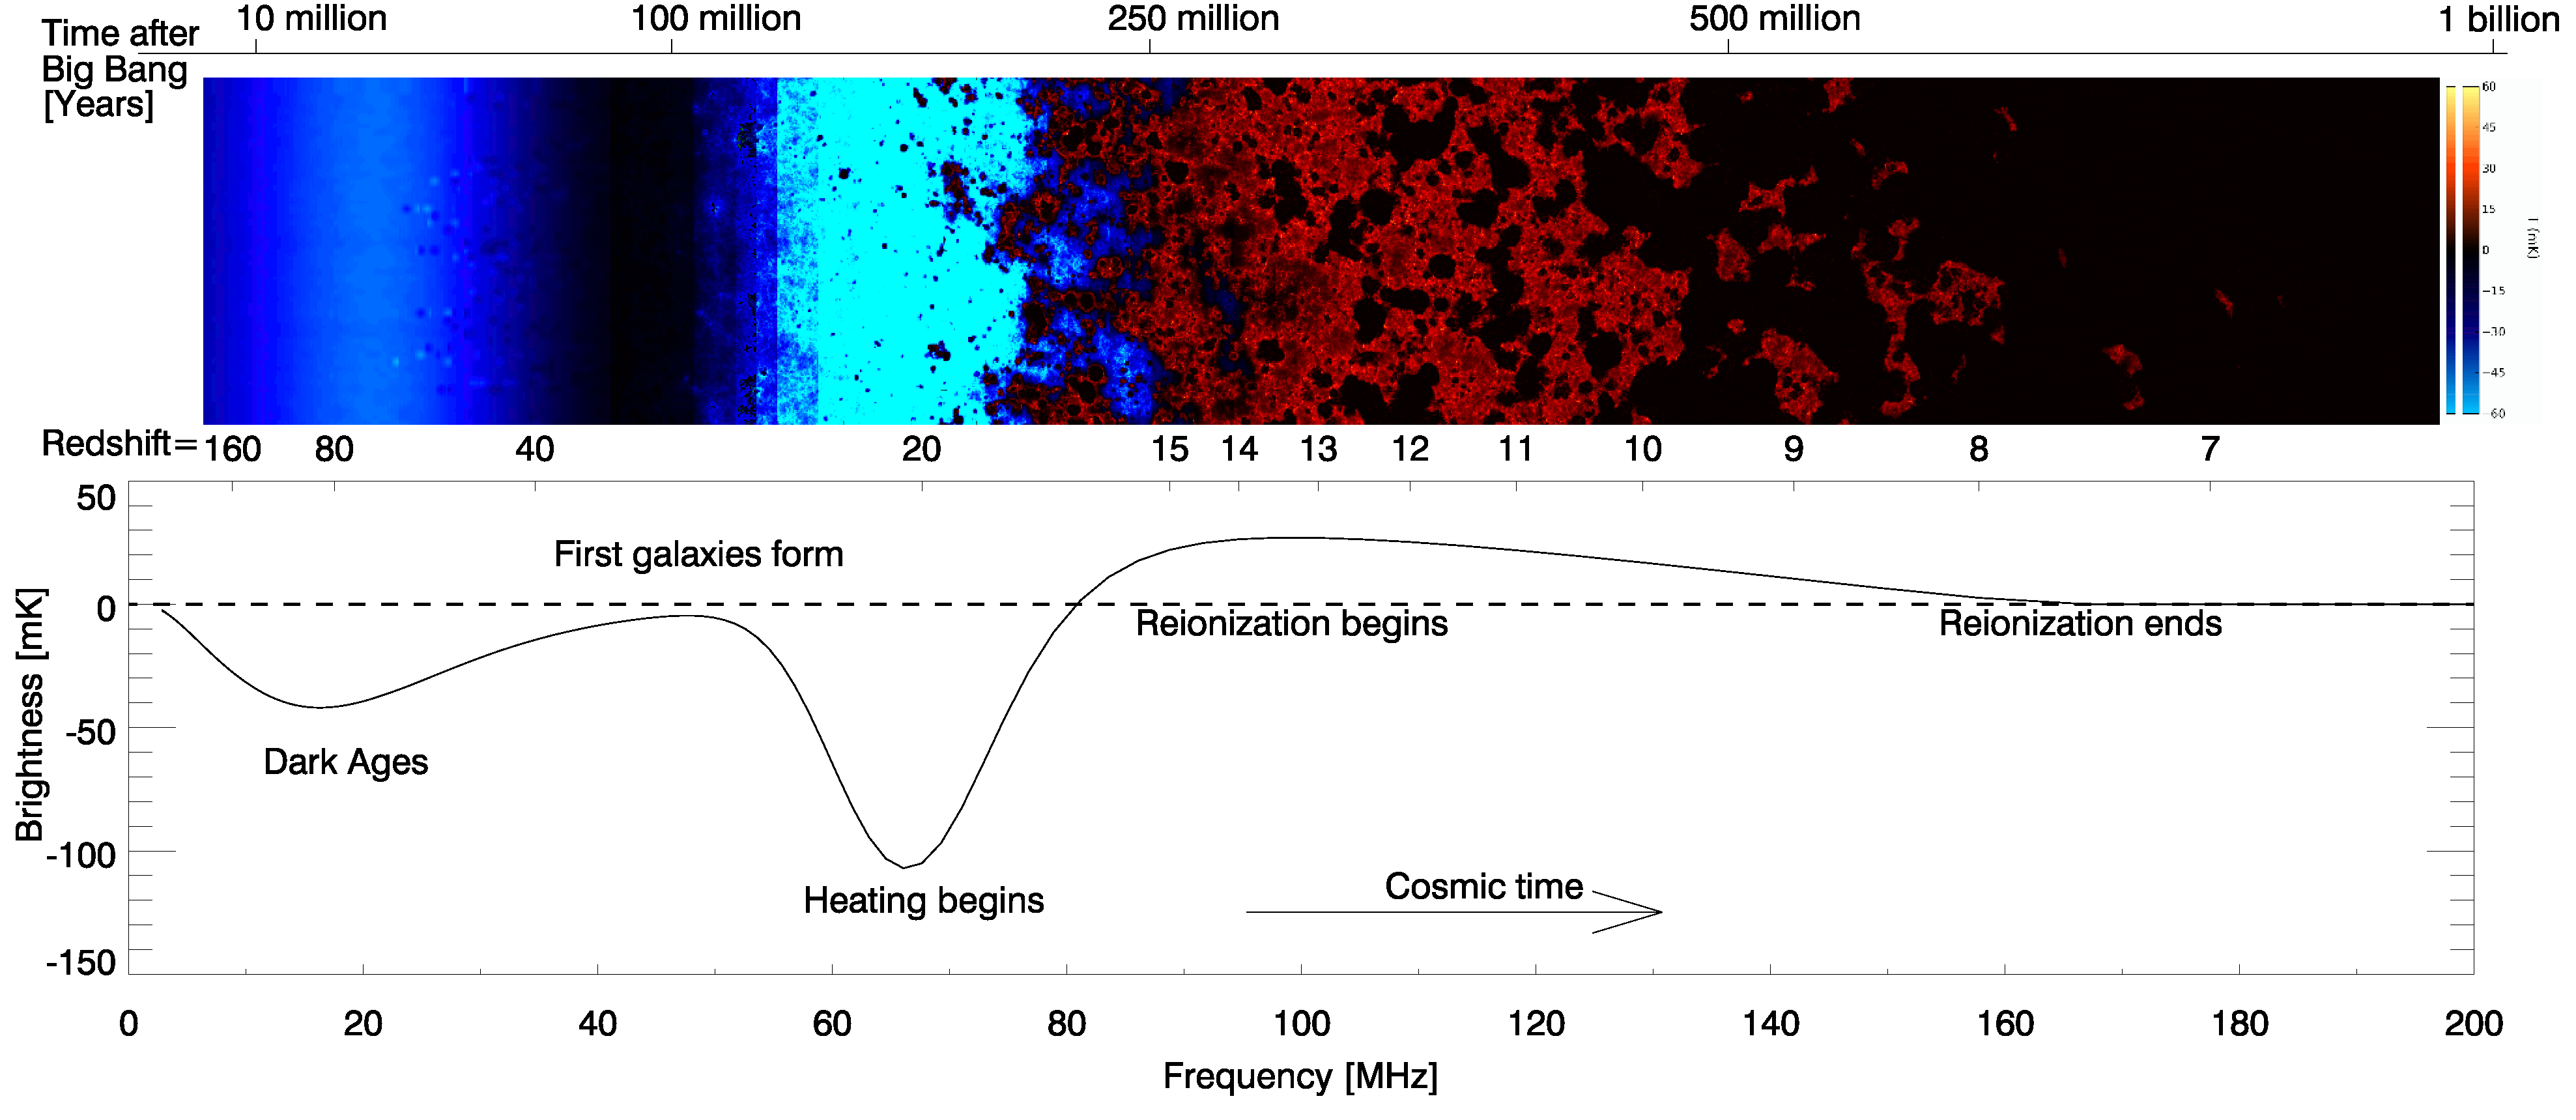
\includegraphics[width=\textwidth]{figures/chapter1/pritchard-2012-global-signal}
    \caption{
        Reproduced from \citet{2012RPPh...75h6901P}.
        get a license to use this figure (hit an error, but email sent (7-7-2018))
    }
    \label{fig:pritchard-global-signal}
\end{figure}

Neutral hydrogen in the early universe is illuminated by the CMB. A calculation of the radiative
transfer \citep{2012RPPh...75h6901P} yields (neglecting the contribution of peculiar velocities):
\begin{equation}\label{eq:radiative-transfer-equation}
    \Delta T_{21} \approx 27 \left[
        \overbrace{
            x_\text{HI} (1+\delta)
            \left(\frac{\Omega_b h}{0.0327}\right)
        }^{\text{quantity of HI}}
        \left(\frac{\Omega_m}{0.307}\right)^{-1/2}
        \left(\frac{1+z}{10}\right)^{1/2} \linebreak \times
        \overbrace{
            \left(\frac{T_\text{spin} - T_\text{CMB}(z)}{T_\text{spin}}\right)
        }^{\text{relative temperature}}
    \right] \, {\rm mK} \,,
\end{equation}
where $\Delta T_{21}$ is the expected 21~cm brightness temperature. If $\Delta T_{21} > 0$, it
appears in emission against the CMB. If $\Delta T_{21} < 0$, it appears in absorption. $x_\text{HI}$
is the neutral fraction of hydrogen, $\delta$ is the local baryon overdensity, $h$ is the Hubble
constant, $\Omega_b$ is the density parameter for baryons, $\Omega_m$ is the density parameter for
matter, $T_\text{spin}$ is the spin temperature (excitation temperature of the 21~cm transition),
and $T_\text{CMB}(z) = 2.73\,(1+z)\,{\rm K}$ is the temperature of the CMB at the redshift $z$.

Equation~\ref{eq:radiative-transfer-equation} is fundamental to determining what can be learned
through detecting the 21~cm transition at high redshift. First, if the spin temperature is greater
than the CMB temperature, the 21~cm transition appears in emission. However, the signal saturates at
high spin temperatures. If the spin temperature is less than the CMB temperature, the 21~cm
transition appears in absorption with no saturation point. Second, the amplitude of the signal is
proportional to the total quantity of \ion{H}{1}. Therefore, in order for there to be a measurable
21~cm signal, the universe must be predominantly neutral, and the transition must not be in
radiative equilibrium with the CMB. An example prediction for $\Delta T_{21}$ can be seen in
Figure~\ref{fig:pritchard-global-signal}.

There are three relevant temperatures that affect the spin temperature: $T_\text{gas}$, the
temperature of the gas, $T_\text{CMB}$, the temperature of the CMB, and $T_{\text{Ly}\alpha}$, the
color temperature of the Ly$\alpha$ radiation from early star formation. More exotic theories might
also include the temperature of the dark matter, $T_\text{DM}$. Generally,  the Ly$\alpha$ photons
scatter through the intergalactic medium (IGM), which sets $T_{\text{Ly}\alpha} = T_\text{gas}$. In
the absence of any heating mechanisms, the matter and radiation are both cooling adiabatically with
the expansion of the universe.  The adiabatic indices are $\gamma = 5/3$ and $\gamma = 4/3$
respectively, so the matter cools faster than the radiation. Consequently, the 21~cm transition
tends to appear in absorption prior to early star formation, and in emission after the IGM has been
heated.

While there are currently few observational constraints on the 21~cm brightness temperature,
fiducial theoretical models tell the following story\todo{add a reference here}.  During the dark
ages ($z \gtrsim 40$) the density of the universe is high enough for collisions between hydrogen
atoms to dominate the excitation of the 21~cm transition.  Consequently during this time
$T_\text{spin} = T_\text{gas}$, and the 21~cm transition appears in absorption against the CMB.
Later ($z \sim 30$), as the mean density of the universe decreases, collisions become more
infrequent and the 21~cm transition is instead excited by CMB photons. During this time the 21~cm
signal vanishes because $T_\text{spin} = T_\text{CMB}$.

With the onset of star formation in the universe, the IGM is inundated with Ly$\alpha$ photons.
These Ly$\alpha$ photons scatter through the IGM. With the absorption and re-emission of a
Ly$\alpha$ photon, a hydrogen atom can transition between the spin-symmetric state and the
spin-antisymmetric state. This process, called the Wouthuysen-Field effect, sets the relative
abundance of \ion{H}{1} in each state such that $T_\text{spin} = T_{\text{Ly}\alpha} = T_\text{gas}$
\citep{1952AJ.....57R..31W,1958PIRE...46..240F}. Therefore, after early star formation begins, the
21~cm transition reappears in absorption against the CMB.

However, as star formation progresses, the gas in the IGM is heated. X-rays are particularly
effective at heating the IGM due to their large mean-free path. Consequently the heating rate is
sensitive to, for example, the number density, luminosity and spectral hardness of X-ray binaries.
Eventually the gas is heated above the temperature of the CMB, bringing the 21~cm transition into
emission, and eventually the signal saturates. At this point the 21~cm
transition begins to disappear with the onset of reionization at $z \lesssim 15$ due to the
disappearance of neutral hydrogen. A prediction of the spectral distortion this process applies to
the low-frequency ($\nu < 200\,\text{MHz}$) CMB spectrum can be seen in the bottom panel of
Figure~\ref{fig:pritchard-global-signal}.









For much of the universe's history, the intergalactic medium (IGM) is ionized or in radiative
equilibrium with the CMB.





Given knowledge of the
original wavelength of the photon, and the expansion history of the universe, we can calculate how
long the photon must have been in flight.


Today the CMB is a 2.7~K sea of photons that permeates the universe. This radiation is constantly
cooling due to the inexorable expansion of the universe.


Introduce low frequency telescopes.

Two different types of experiments are currently being designed to target the high-redshift 21~cm
transition:
\begin{enumerate}
    \item single antenna experiments that are attempting to measure the sky-averaged 21~cm signal,
        and
    \item large interferometers that are attempting to measure the three-dimensional spatial power
        spectrum of the 21~cm signal.
\end{enumerate}
Both types require exquisite calibration and roughly five orders of dynamic range against the
blindingly bright foreground radio emission, but are subject to different (but not exclusively
different) systematic instrumental errors.

Likely the most substantial challenge faced by both classes of experiments is the existence of
foreground radio emission. At large angular scales $\theta \gg 1\arcdeg$, the radio sky is dominated
by galactic synchrotron emission generated by relativistic electrons spiralling around galactic
magnetic field lines. The EDGES experiment, in the southern hemisphere, measured the brightness
temperature of this emission to be \citep{2017MNRAS.464.4995M}
\begin{equation}\label{eq:edges-sky-spectrum}
    T \sim 300\,{\rm K} \times \left(\frac{\nu}{150\,{\rm MHz}}\right)^{-2.6}\,.
\end{equation}
At smaller angular scales $\theta \lesssim 1\arcdeg$, the galactic emission gives way to a sea of
active galactic nuclei (AGN), the brightest of which, Cyg A, has a flux $>15,000\,\text{Jy}$ at
frequencies $<80\,\text{MHz}$ \citep{1977A&A....61...99B}. A simple comparison between
Equations~\ref{eq:radiative-transfer-equation} and \ref{eq:edges-sky-spectrum} reveals that the
foreground radio emission must be suppressed by four to five orders of magnitude.  However, this
foreground emission is typically synchrotron and free-free, which are both spectrally smooth. The
21~cm signal, on the other hand, is not expected to be so smooth. This is due to the fact that
sweeping through frequency along a line of sight probes different causally disconnected regions of
the universe. Each of these regions experiences a different star formation, heating and reionization
history, which ultimately produces a different 21~cm brightness temperature.  However, at the same
time there is a relative paucity of suitable modern, high-fidelity sky maps at these frequencies.

Global-signal experiments have no intrinsic angular resolution of their own. To date, these
experiments have typically relied on low-order polynomial fits to remove the foreground
contamination in their measurements. This is a fine balancing routine, because if the polynomial
order is chosen to be too low, residual foreground contamination dominates the measurement. If the
polynomial order is chosen to be too high, the 21~cm signal itself can be removed.

\begin{figure}[t]
    \centering
    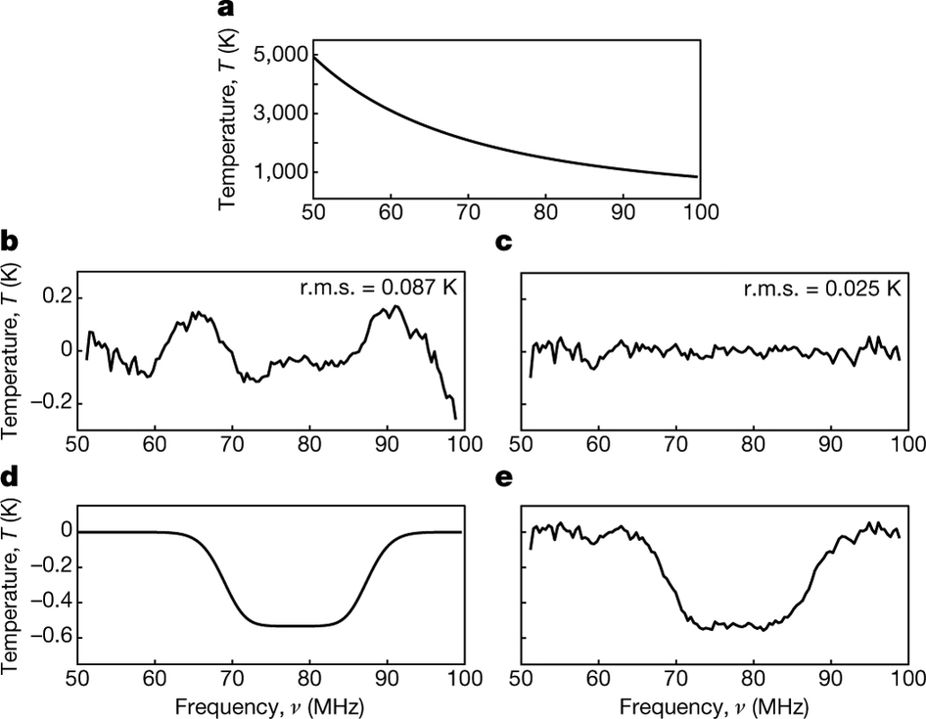
\includegraphics[width=\textwidth]{figures/chapter1/bowman-2018-absorption-trough}
    \caption{
        Reproduced from \citet{2018Natur.555...67B}.
        the Nature thing to get permission for this figure kept redirecting me to a blank page while
        I was trying to fill out the form. Why are all of these things garbage? Still, I need to get
        permission for this figure...
    }
    \label{fig:bowman-absorption-trough}
\end{figure}

Recently, a significant development came from the first putative detection of the global 21~cm
signal by the EDGES experiment \citep{2018Natur.555...67B}. In this paper, the authors claimed a
detection of an absorption feature centered at $78\,\text{MHz}$, which they attribute to early star
formation and heating (see Figure~\ref{fig:bowman-absorption-trough}). If true, this detection is
remarkable for its extreme $\sim500\,\text{mK}$ amplitude. In order to generate such a large
absorption feature, either the IGM needs to be cooled below temperatures it is possible to reach
purely through adiabatic cooling, or an additional source of radio emission must be present at $z >
20$.

\begin{figure}[t]
    \centering
    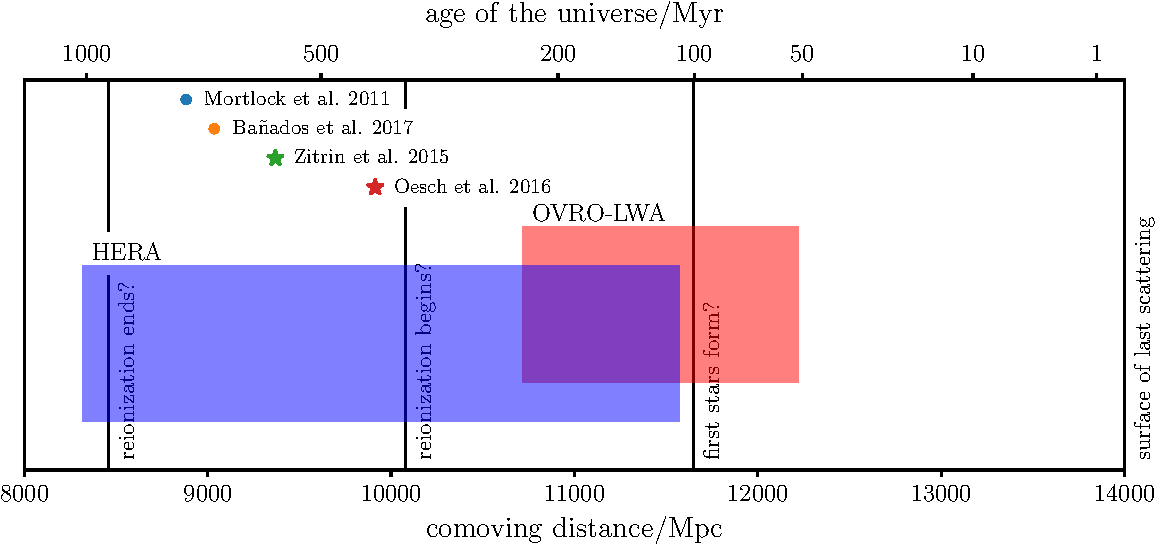
\includegraphics[width=\textwidth]{figures/chapter1/history-of-the-universe/history-of-the-universe}
    \caption{
        A radial map of the universe. Known quasars are marked with circles and galaxies are marked
        with stars. The range of comoving distances probed by the OVRO-LWA and HERA are marked with a red
        rectangle and a blue rectangle respectively.
    }
    \label{fig:history-of-the-universe}
\end{figure}

\begin{figure}[t]
    \centering
    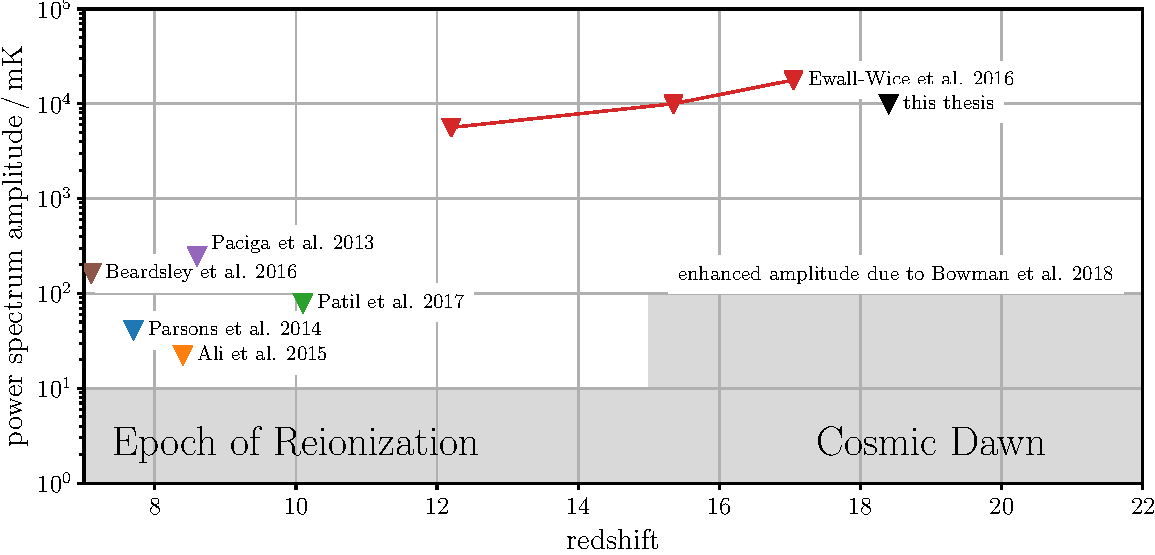
\includegraphics[width=\textwidth]{figures/chapter1/power-spectrum-upper-limits/power-spectrum-upper-limits}
    \caption{
        Power spectrum amplitude upper limits (95\% confidence) as a function of redshift. The
        shaded region denotes roughly where current theoretical predictions fall.
    }
    \label{fig:power-spectrum-upper-limits}
\end{figure}












\myputbib{thesis}
\end{bibunit}


\cleartoevenpage

\myepigraph
{This is radio astronomy!}
{Tony Readhead}

\chapter{A Path Towards Calibration of the OVRO-LWA}
\label{chapter2}

\begin{bibunit}

\section{Design and Construction of the OVRO-LWA}

\begin{figure}
    \centering
    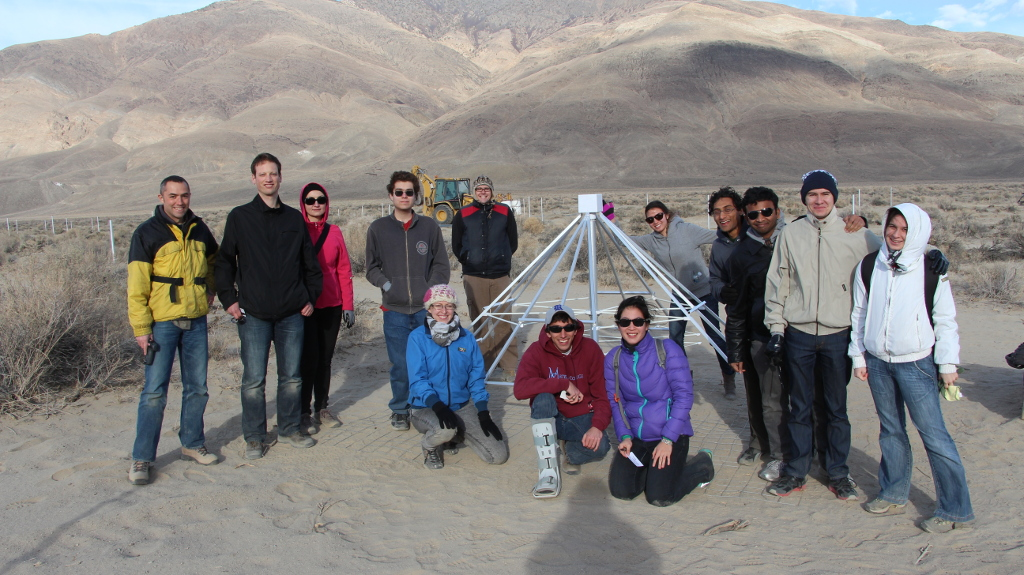
\includegraphics[width=\textwidth]{figures/chapter2/first-antenna}
    \caption{
        The first OVRO-LWA completed on 2013 March 8 with the class of Ay~122b (including the author
        of this thesis with the fractured ankle).
    }
    \label{fig:ovro-first-antenna}
\end{figure}

\begin{figure}
    \centering
    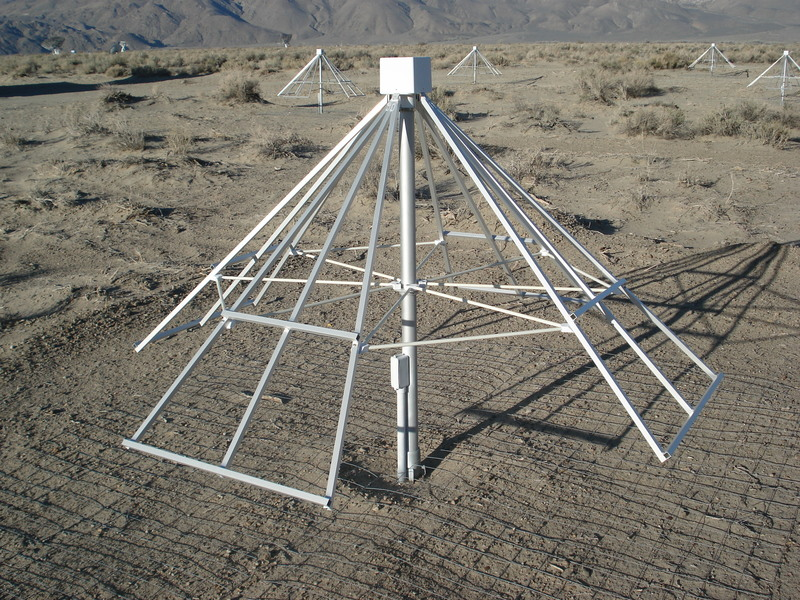
\includegraphics[width=\textwidth]{figures/chapter2/lwa-antenna}
    \caption{
        Picture of an OVRO-LWA antenna.
    }
    \label{fig:ovro-lwa-pictures}
\end{figure}

The OVRO-LWA is a new low-frequency (27--85\,MHz) radio interferometer constructed during the course
of this thesis and located near Big Pine, California. Construction began in 2013 with the first
antenna completed in March of that year (see Figure~\ref{fig:ovro-first-antenna}).

The OVRO-LWA was initially composed of 256 antennas, with 251 of those antennas arranged within a
dense 200\,m diameter core in a configuration that is optimized for sidelobe levels in snapshot
imaging.  Each of these antennas consists of two crossed broadband dipoles with an active
balun/preamp, and the entire system is sky noise dominated over the range 20--80\,MHz
\citep{2012PASP..124.1090H}.  A picture of an OVRO-LWA antenna can be seen in
Figure~\ref{fig:ovro-lwa-pictures}. The primary beam of each OVRO-LWA antenna subtends a solid angle
of $\sim 8000\,\text{deg}^2$, with sensitivity to the entire visible hemisphere of the sky.

%\todo{ARX boards}

The remaining five antennas are isolated from the core of the OVRO-LWA and equipped with radiometric
front ends as part of the LEDA experiment, which is attempting to measure the globally averaged
signal of \ion{H}{1} from the Cosmic Dawn \citep{2018MNRAS.478.4193P}.  The OVRO-LWA hosts the LEDA
correlator as its back-end, which is an FX correlator composed of 16 ROACH2 FPGAs that form the F
stage, and 11 servers each with dual NVIDIA K20X GPUs that form the X stage
\citep{2015JAI.....450003K}. This allows the correlator to perform full cross-correlation of 512
input signals with 58\,MHz instantaneous bandwidth.

During observations, data is streamed from the LEDA correlator to the All-Sky Transient Monitor
(ASTM), which houses the compute nodes used for post-processing and imaging.  The ASTM is composed
of 10 identical nodes each with a 16-core Intel Xeon E5-2630 v3 CPU and 64\,GB of memory. Five
additional servers provide 565\,TB of storage capacity through the Lustre high performance file
system.

The initial 256 antenna interferometer was therefore capable of imaging the entire visible
hemisphere in snapshot images with 1$\arcdeg$ angular resolution. An example snapshot image can be
seen in Figure~\ref{fig:core-snapshot-image}.  In 2015, an additional 32 antennas were installed
that extended the maximum baseline of the interferometer to 1.5\,km and improved the angular
resolution to 8$\arcmin$. This improved angular resolution can be seen in
Figure~\ref{fig:expansion-snapshot-image}. In a final future stage of development, an additional 64
antennas will be installed that extend the maximum baseline to 2.6\,km, which will see improved
$uv$-coverage at long baselines and improved $5\arcmin$ angular resolution, as well as an expanded
correlator to accommodate the additional antennas.

While this thesis focuses on the use of the OVRO-LWA to detect the high-redshift signature of
neutral hydrogen from the Cosmic Dawn, the OVRO-LWA facilitates a diverse set of scientific
motivations including the study of stellar and planetary magnetospheres, radio follow-up of neutron
star mergers and gamma ray bursts \citep{2017arXiv171106665A}, solar dynamic imaging spectroscopy,
and the detection of high energy cosmic rays \citep{caltechthesis11016}.

With the exception of detecting high energy cosmic rays---which uses a custom firmware and
processing pipeline that currently cannot operate in parallel with ordinary correlation---there are
two complementary software pipelines that service the scientific goals of the OVRO-LWA:
\begin{enumerate}
    \item A widefield snapshot imaging pipeline that images the entire visible hemisphere every
        13\,s using \texttt{WSCLEAN} \citep{2014MNRAS.444..606O}.
    \item A novel approach, called $m$-mode analysis, that is specialized for drift-scanning
        interferometers that can image the entire sky (above a limiting declination) in a single
        synthesis imaging step.
\end{enumerate}
This chapter will describe the calibration and source removal routines purpose built for the
OVRO-LWA and used by both pipelines. Additionally, in \S\ref{sec:commissioning-challenges} I will
discuss some of the challenges involved with commissioning the OVRO-LWA that have been overcome to
bring the OVRO-LWA into existence, to first light, and finally its first scientific results.
Finally, the latter pipeline will be discussed in considerable depth in Chapters~\ref{chapter3} and
\ref{chapter4}.

\begin{figure}[p]
    \centering
    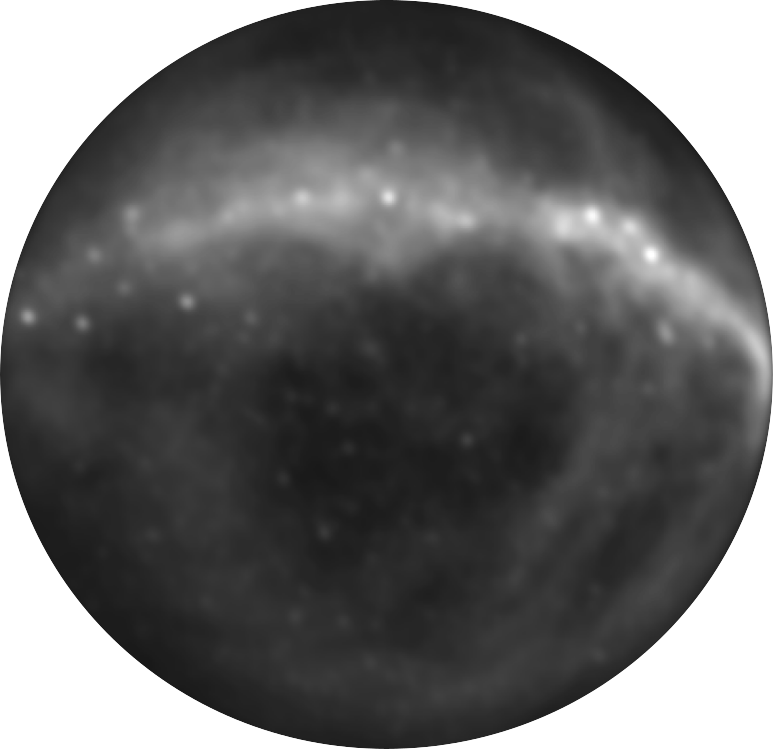
\includegraphics[width=\textwidth]{figures/chapter2/before-expansion}
    \caption{
        Snapshot image of the sky captured with the OVRO-LWA and using only the antennas located
        within the core of the array. The image covers the entire visible hemisphere in
        sine-projection.  A similar image constructed using the newer long-baseline antennas can be
        seen in Figure~\ref{fig:expansion-snapshot-image}.
    }
    \label{fig:core-snapshot-image}
\end{figure}

\begin{figure}[p]
    \centering
    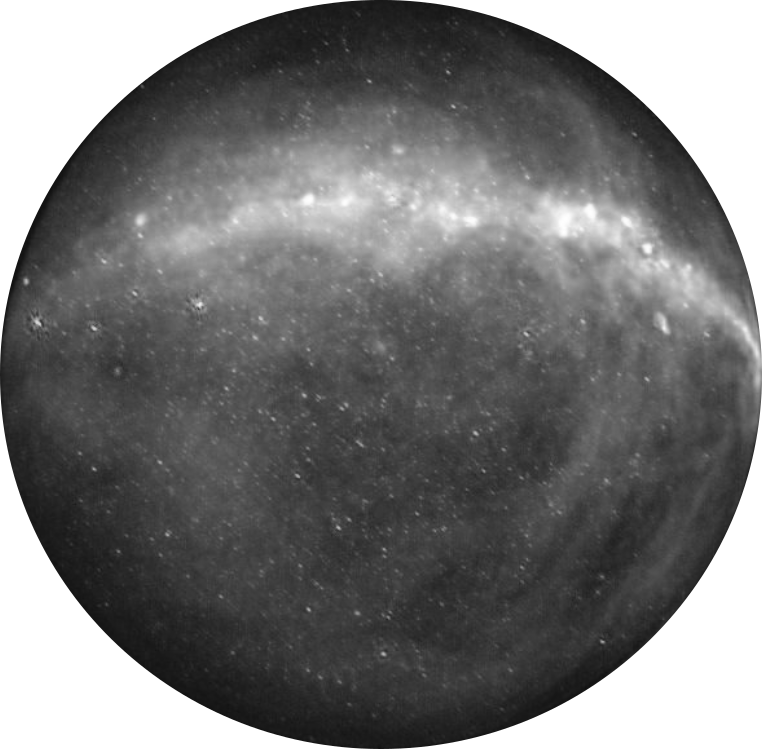
\includegraphics[width=\textwidth]{figures/chapter2/after-expansion}
    \caption{
        Snapshot image of the sky captured with the OVRO-LWA and using the new long-baseline
        antennas. The image covers the entire visible hemisphere in sine-projection.  A similar
        image constructed using only the core of the interferometer can be seen in
        Figure~\ref{fig:core-snapshot-image}.
    }
    \label{fig:expansion-snapshot-image}
\end{figure}

\section{Calibration of a Low-Frequency Interferometer}\label{sec:gain-calibration}

The purpose of calibration is to remove the contribution of the antenna and receivers, including any
gain, filters, and propagation effects along the signal path. At low radio frequencies, the Earth's
ionosphere is additionally important due to the effects of electromagnetic waves propagating through
a magnetized plasma.

We will make a distinction between a ``direction-independent'' calibration and a
``direction-dependent'' calibration. The former can correct for the response of the receiver and
signal path, but cannot fully account for the antenna response pattern and ionospheric effects. The
latter allows for the calibration parameters to vary as a function of direction on the sky, which
can account for errors due to the antenna beam and some ionospheric effects.

Neglecting complexity associated with polarized imaging, a direction-independent calibration amounts
to determining the complex-valued gain $g_i(\nu)$ associated with each signal path $i$ and frequency
$\nu$. These gains effect the measured correlation between the signal paths $i$ and $j$ such that
\begin{equation}
    V_{ij}^\text{measured}(\nu) = g_i(\nu)\,g_j^*(\nu)\,V_{ij}^\text{true}(\nu)
        + \text{noise}\,,
\end{equation}
where $V_{ij}^\text{measured}$ is the visibility actually measured between the corresponding signal
paths at the frequency $\nu$, and $V_{ij}^\text{true}$ is the visibility that would have been
measured if instead we had correlated the value of the electric field at the electrical center of
each antenna without the need for any additional electronics. The true visibility
can be computed from the sky brightness $I(\nu, \hat{r})$ at the
frequency $\nu$ and direction $\hat r$ such that
\begin{equation}
    V_{ij}^\text{true}(\nu) = \int a_i(\nu, \hat{r})\,a_j^*(\nu, \hat{r})\,I(\nu, \hat{r})\,
        \exp\Big(2\pi i\hat{r}\cdot\vec{b_{ij}}/\lambda\Big)\,\d\Omega,
\end{equation}
where the integral runs over solid angle $\Omega$, $a_i(\nu, \hat{r})$ is the response of the
corresponding antenna at the frequency $\nu$ to the direction $\hat{r}$, $\vec{b_{ij}}$ is the
baseline separating the antennas for signal paths $i$ and $j$, and $\lambda$ is the wavelength.  If
the sky is assumed to be composed of point sources, then
\begin{equation}\label{eq:antenna-response-point-sources}
    V_{ij}^\text{true}(\nu) = \sum_k a_i(\nu, \hat{r}_k)\,a_j^*(\nu, \hat{r}_k)\,F_k(\nu)\,
        \exp\Big(2\pi i\hat{r}_k\cdot\vec{b_{ij}}/\lambda\Big)\,,
\end{equation}
where $F_k$ is the flux of the $k$th point source in the direction $\hat{r}_k$.

A typical calibration strategy using, for example, the Very Large Array (VLA) involves periodically
pointing at a known compact point source. For a compact point source at the phase center, the phase
of each visibility is zero, and the amplitude is given by the known flux of the source.
Periodically revisiting this source allows for the observer to establish the time variation of the
calibration parameters by solving for the gains that minimize
\begin{equation}
    \chi^2 \propto \sum_{i, j}
        \Big\|V_{ij}^\text{measured}(\nu) - g_i(\nu)\,g_j^*(\nu)\,F\Big\|^2\,,
\end{equation}
where $F$ is the flux of the isolated point source.

This optimization can be performed with rapid convergence using a variant of alternating
least-squares developed by \citet{2008ISTSP...2..707M} and \citet{2014A&A...571A..97S}. At each
iteration this algorithm applies linear least-squares to minimize $\chi^2$ while holding one set of
gains constant:
\begin{equation}\label{eq:stefcal-iterations}
    g_i \leftarrow \frac
        {\sum_{j\neq i} g_j^* V_{ij}^{\text{model},*} V_{ij}^\text{measured}}
        {\sum_{j\neq i} \| g_j V_{ij}^\text{model} \|^2}\,,
\end{equation}
where we have now allowed for a more general sky model to be used during calibration by introducing
the model visibilities $V_{ij}^\text{model}$, which are the true visibilities for an assumed model
of the sky.  Naively applying Equation~\ref{eq:stefcal-iterations} will result in poor convergence
due to oscillations about a minimum of $\chi^2$.  These oscillations can be damped by averaging
subsequent iterations, and \citet{2014A&A...571A..97S} demonstrated that this simple gradient-free
optimization strategy converges remarkably quickly.

The OVRO-LWA is capable of imaging the entire hemisphere in a snapshot image. This brings its own
unique calibration challenges because it is currently impossible to isolate a single compact point source
within the field of view of the interferometer.\footnote{
    Gated pulsar observations could, in principle, achieve this isolation. This capability is a key
    development area for the OVRO-LWA.
}
Due to the wide field of view, determining an accurate gain calibration relies on a detailed sky and
antenna beam model. Mistakes or omissions in the sky model can, for example, generate artificial
ripples in the bandpass that will impact the interferometer's ability to cleanly separate foreground
emission from cosmological 21~cm emission \citep{2016MNRAS.461.3135B, 2017MNRAS.470.1849E}.

Furthermore, at frequencies $\nu < 100\,\text{MHz}$ there are few flux calibrators.
\citet{1977A&A....61...99B} determined the absolute spectrum of Cyg~A between 20~MHz and 2~GHz.
\citet{2012MNRAS.423L..30S} added six additional calibrators, and \citet{2017ApJS..230....7P} used
the VLA 4-band system to bring the total number of available calibrators to 11. However, in
Chapter~\ref{chapter3} I will show that the latter spectra can diverge substantially from truth
when extrapolated below 50~MHz.

Detailed sky and beam models are therefore generally an important calibration requirement for
low-frequency interferometers.  In Chapter~\ref{chapter3}, I will derive an empirical beam model for
the OVRO-LWA and develop a new imaging formalism that captures the entire visible sky in a single
synthesis imaging step that can be used as part of a self-calibration loop
\citep{1978ApJ...223...25R}.

As part of this thesis I developed the \texttt{TTCal} calibration routine for the purpose of
calibrating the OVRO-LWA. It implements the alternating least-squares algorithm described above to
solve for the complex-valued gain of each signal path from a model sky composed of any number of
point sources, Gaussians, and shapelet components \citep{2003MNRAS.338...35R}. If desired,
\texttt{TTCal} may instead solve for the Jones matrix associated with each antenna for a fully
polarized calibration solution. \texttt{TTCal} is freely available under the GPLv3 license or under
any later version.\footnote{
    \url{https://github.com/mweastwood/TTCal.jl}
}

%Some interferometers (e.g., HERA and the MWA), recognizing the difficulty of gain calibration at low
%frequencies, have opted for partly redundant antenna configurations. These configurations can solve
%for many of their calibration parameters internally without relying on an incomplete sky model and
%potentially inaccurate antenna beam model \citep{2010MNRAS.408.1029L}. However, these
%interferometers sacrifice imaging fidelity, which is useful for establishing the remaining
%calibration parameters (e.g., the overall bandpass cannot be solved for in an internal
%redundant-calibration routine).

\section{Source Removal and Direction-Dependent Calibration}

\begin{figure}
    \centering
    \begin{tabular}{ccc}
        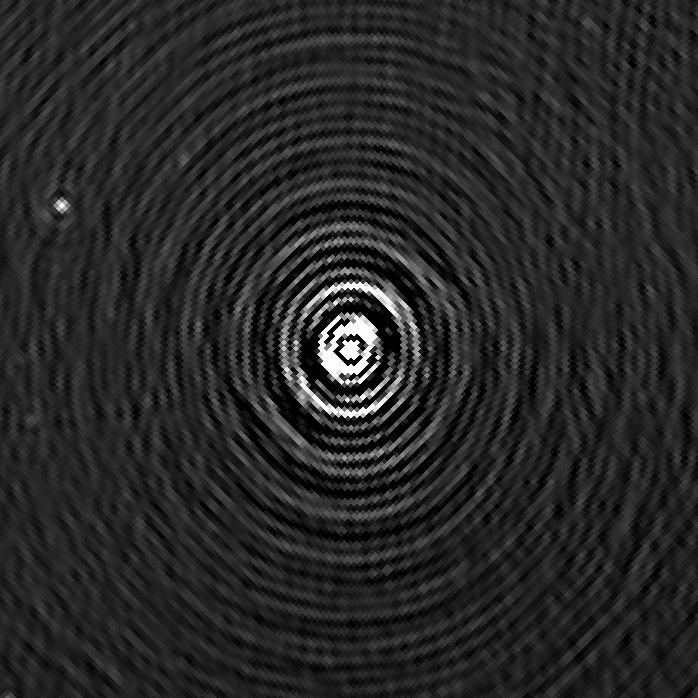
\includegraphics[width=0.3\textwidth]{figures/chapter2/cas-a-no-removal} &
        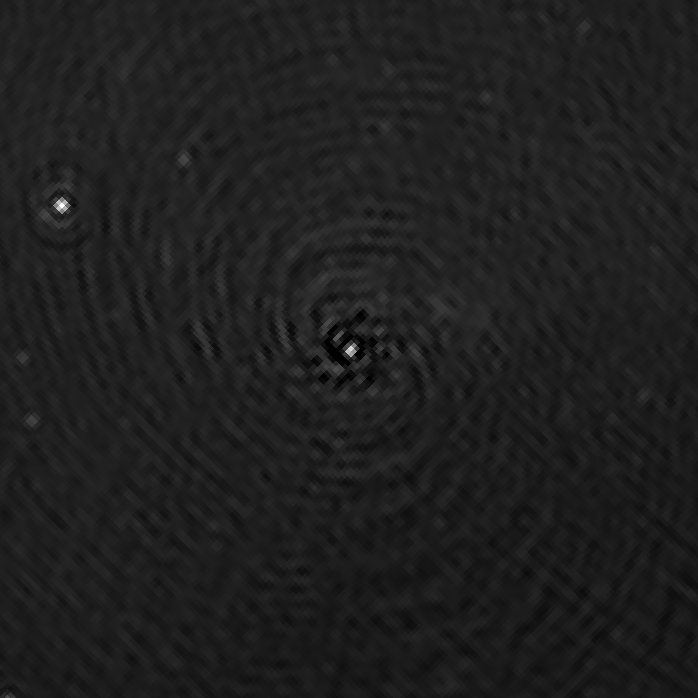
\includegraphics[width=0.3\textwidth]{figures/chapter2/cas-a-subtraction} &
        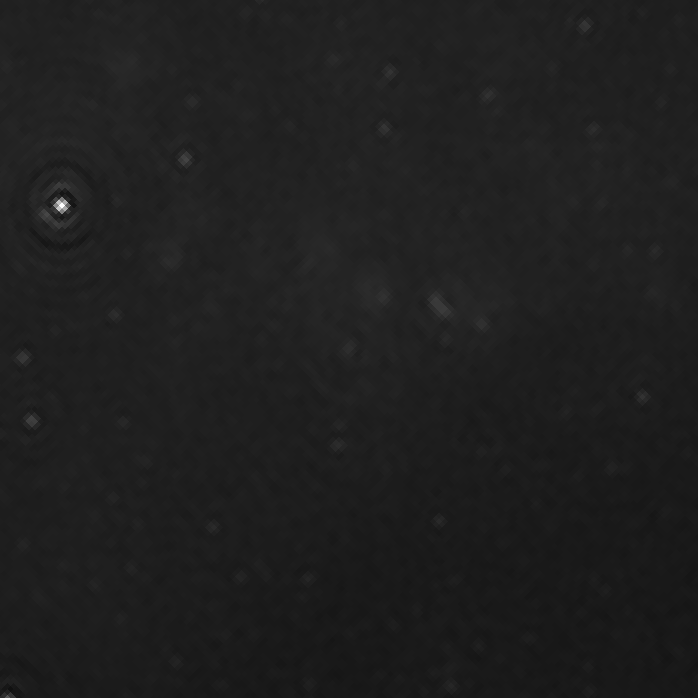
\includegraphics[width=0.3\textwidth]{figures/chapter2/cas-a-peeling} \\
        (a) & (b) & (c) \\
    \end{tabular}
    \caption{
        Illustration of the improvement in source removal associated with peeling using
        \texttt{TTCal}. (a) Image of Cas~A prior to source removal. (b) Image of Cas~A after
        subtracting a point source without the application of direction-dependent gains. (c) Image
        of Cas~A after peeling (including the application of direction-dependent gains).
    }
    \label{fig:peeling-illustration}
\end{figure}

The large field of view of the OVRO-LWA comes with additional challenges associated with the
ionosphere, inhomogeneous primary beams, and mutual coupling between antennas.

The dispersion relation for electromagnetic waves propagating in a plasma is
\begin{equation}
    \omega^2 = \omega_\text{plasma}^2 + c^2 k^2\,,
\end{equation}
where $\omega$ is the angular frequency of the oscillations, $k$ is the wavenumber, $c$ is the speed
of light, and $\omega_\text{plasma}$ is the plasma frequency---the frequency of electrostatic
oscillations within the plasma. The plasma frequency (in SI units) is given by
\begin{equation}
    \omega_\text{plasma} = \sqrt{\frac{n_e e^2}{m_e \varepsilon_0}}\,,
\end{equation}
where $n_e$ is the number density of electrons, $e$ is the charge of the electron, $m_e$ is the mass
of the electron, and $\varepsilon_0$ is the permittivity of free space.  For Earth's ionosphere, the
plasma frequency is typically $\sim 2\pi \times 10\,\text{MHz}$.  The index of refraction is
\begin{equation}
    n = \sqrt{1 - \frac{\omega_\text{plasma}^2}{\omega^2}}
      \approx 1 - \frac{1}{2}\frac{\omega_\text{plasma}^2}{\omega^2}\,,
\end{equation}
where the approximation holds if $\omega^2 \gg \omega_\text{plasma}^2$. In this regime, the arrival
time of a burst of radio emission is $\propto \nu^{-2}$, as is commonly seen in pulsar astronomy.
The additional phase imparted is, however, $\propto \nu^{-1}$ such that along a given line of sight
the phase can be parameterized as
\begin{equation}
    \phi \approx \phi_0 + \overbrace{2\pi\tau\nu}^\text{delay}
    + \overbrace{\frac{e^2}{4\pi m_e c \varepsilon_0}
        \frac{1}{\nu}\int n_e\,\d l}^\text{ionospheric dispersion}\,,
\end{equation}
where $\phi_0$ sets the overall phase, $\tau$ is the delay, and the integral of the electron number
density along the line of sight is called the Total Electron Content (TEC).

The diffractive scale $r_\text{diff}$ of the ionosphere is the length scale over which the phase
variance is $1\,\text{rad}^2$. Approximately 90\% of the time the diffractive scale is
$>2\,\text{km}$ at 70\,MHz and $>1\,\text{km}$ at 35\,MHz \citep{2016RaSc...51..927M}.  The Fresnel
scale is $r_\text{f} = \sqrt{\lambda D / 2\pi}$ where $D$ is the height of the ionosphere (typically
$\sim 300\,\text{km}$). In the weak scattering regime ($r_\text{diff} \gg r_\text{f}$), the
ionosphere can contribute amplitude and phase scintillation, which may be folded into the antenna
gain calibration.  However, in the strong scattering regime ($r_\text{diff} \lesssim r_\text{f}$),
point sources may become multiply imaged, which cannot be described as a perturbation to the antenna
response \citep{2015MNRAS.453..925V}. Typically the OVRO-LWA operates in the weak scattering regime,
with baselines shorter than the diffractive scale of the ionosphere.

A compact interferometer is composed of antennas that are staring through the same patch of the
ionosphere. The ionosphere therefore imparts a phase gradient across the array that refracts sources
from their true position.  In contrast, on longer baselines, the additional phase between the two
antennas may not be correlated \citep{2005ASPC..345..399L}.

However, the antenna response is also generally expected to be inhomogeneous.  Within the core of
the OVRO-LWA, antennas are separated by as little as 5\,m.  \citet{2011ITAP...59.1855E} studied the
impact of mutual coupling on the antenna primary beam within the first Long Wavelength Array station
in New Mexico (LWA1), which uses the same antennas and same 5\,m minimum spacing as the OVRO-LWA,
but the antennas are packed within a 100\,m diameter (as opposed to a 200\,m diameter for the
OVRO-LWA). The authors found that, between 20--74\,MHz, when pointing more than
10$\arcdeg$--20$\arcdeg$ from zenith, mutual coupling and correlated galactic noise led to a
2--6\,dB increase in the system equivalent flux density (SEFD), and 1--2\,dB deviations in the
primary beam pattern between antennas. We expect comparable effects for the OVRO-LWA.

Direction-dependent calibration therefore attempts to account for ionospheric scintillation and
refraction, as well as inhomogeneous antenna beams, by allowing the antenna response in
Equation~\ref{eq:antenna-response-point-sources} to be a free parameter.  \texttt{TTCal} implements
direction-dependent calibration during source subtraction in an algorithm known as peeling
\citep{2008ISTSP...2..707M}. Figure~\ref{fig:peeling-illustration} illustrates the improvement
associated with applying direction-dependent gains during the subtraction of Cas~A---one of the two
brightest point sources in the sky.

\section{Commissioning Challenges}
\label{sec:commissioning-challenges}

\subsection{Computing Antenna Positions}

\begin{figure}
    \centering
    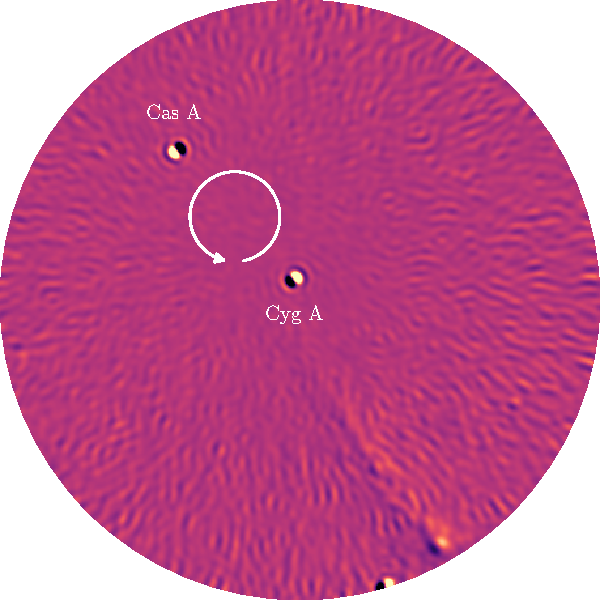
\includegraphics[width=0.7\textwidth]{figures/chapter2/northing-easting-mistake/northing-easting-mistake}
    \caption{
        Illustration of the error in the WCS prior to a correction to the antenna positions. The
        image is a difference between an image constructed with the incorrect antenna positions and
        the corrected antenna positions. The arrow denotes the direction and approximate center of
        the rotation.
    }
    \label{fig:northing-easting-mistake}
\end{figure}

Early images produced by the OVRO-LWA (prior to 2015 October 16) were afflicted by an apparent
rotation in the World Coordinate System (WCS). This rotation is illustrated in
Figure~\ref{fig:northing-easting-mistake}.

When data is streamed to the ASTM, it arrives in a raw, unordered format specific to the operation
of the correlator. The very first step in any analysis is to convert from this format into the
standard \texttt{MeasurementSet} format, which is used by, for example, the National Radio Astronomy
Observatory's (NRAO) Common Astronomy Software Applications (CASA) package. This data conversion
step is performed by the \texttt{dada2ms} program written by Stephen Bourke. As part of this
conversion process, \texttt{dada2ms} computes and attaches additional metadata such as the antenna
positions, frequency of the observations, and the direction of the phase center. Unfortunately an
error had been made in the calculation of the antenna positions.

While many astronomers are familiar with a wide range of celestial coordinate systems, Earth
coordinate systems are somewhat more esoteric. In particular, there are differences between geodetic
systems that seek to describe positions across the entire Earth and those that only seek to describe
positions on a single continental plate. The former geodetic systems are useful, as they specify an
absolute position on the surface of the Earth, while the latter geodetic systems are insensitive to
continental drift and therefore do not naturally change with time. The OVRO-LWA antenna positions
were surveyed in the geodetic system specified by the North American Datum of 1983 (NAD\,83), and
reported in the Universal Transverse Mercator (UTM) coordinate system. NAD\,83 was designed to
closely match the World Geodetic System of 1984 (WGS\,84), and the difference between the two is
generally too small to be of concern to long wavelength radio astronomy (the error in using them
interchangeably is of order one meter in the absolute position of the interferometer).

The UTM coordinate system is described by the coordinate values northing and easting, each measured
in units of meters.  The UTM coordinate system is designed to be a square grid on the surface of a
sphere. This is in contrast to the more familiar latitude and longitude, where a change in longitude
corresponds to a smaller physical distance at high latitudes. Instead, a 1\,km change in easting
corresponds to a physical distance of approximately 1\,km regardless of the position of the
measurement. Consequently, a line of constant easting cannot run true north. Initial calculations of
the OVRO-LWA antenna positions had erroneously assumed that northing runs true north, and easting
runs true east.\footnote{
    Incidentally, the OVRO-LWA is not the first (or the last) interferometer to fall victim to this
    pitfall. The MWA suffered from this mistake during commissioning, and the CHIME pathfinder was
    mistakenly built with its cylindrical focusing surfaces slightly rotated from true north (as was
    the intention).
}

All told, the impact of this mistake was an erroneous $\sim 1\arcdeg$ rotation about zenith in the
antenna positions. Cyg~A and Cas~A, as the brightest point sources in the northern hemisphere at low
radio frequencies, are used to derive the phase calibration of the interferometer. Because the
antenna positions were erroneous, the phase calibration attempts to correct the position of Cyg~A
and Cas~A by applying a phase gradient across the array such that the two sources match their
catalog positions as closely as possible. Images produced by the interferometer therefore appeared
to be rotated by $\sim 1\arcdeg$ about a position roughly between the location of Cyg~A and Cas~A
during calibration. This offset of the rotation center can be seen in
Figure~\ref{fig:northing-easting-mistake}.

I fixed the erroneous calculation of antenna positions by patching \texttt{dada2ms} to stop relying
on the assumption that northing runs true north and easting runs true east. After applying this
patch, \texttt{dada2ms} now correctly converts from the surveyed NAD\,83 UTM coordinate values to
WGS\,84 longitude--latitude values, and finally to the International Terrestrial Reference Frame
(ITRF) using a conversion routine provided by the \texttt{casacore} software package.  In addition,
I discovered a similar coordinate rotation in sky maps generated by the first Long Wavelength Array
(LWA1) station located in New Mexico \citep{2017MNRAS.469.4537D}. Working in collaboration with the
authors of those sky maps, the corrected LWA1 sky maps are now publicly available online.

\subsection{Frequency Channel Labeling}

After correcting the calculation of antenna positions, we achieved improved agreement between
apparent source positions and their catalog positions. However, there was still a residual
systematic error apparent in images constructed during 2015 December. In these images, sources
appeared to be radially offset from the position of Cyg~A and Cas~A.

The ionosphere is a natural culprit because refraction due to propagation through the ionosphere
will tend to move sources to higher elevation \citep[e.g.,][]{2014MNRAS.437.1056V}. Confusingly, the
sense of the observed source offsets was opposite to the expectation of the ionosphere. Sources
appeared at lower elevations than expected. It appeared as if the length of each baseline was
somehow 0.3\% longer than expected.

Such an error could arise due to a mistake in the survey of the antenna positions or another error
in the calculation of their ITRF coordinates. Alternatively, because the action of an interferometer
is dependent on the ratio of the baseline length to the wavelength, the error could be generated by
a mislabeling of the frequency channels output by the correlator. I found that a frequency offset of
$\sim 100\,\text{kHz}$ could be enough to explain the residual source offsets seen in Cyg~A and
Cas~A. Ryan Monroe later confirmed that the error was in the correlator by examining the frequency
of an FFT artifact that arises from the sampling frequency and therefore is a known spectral
feature. This feature was offset from its true location by $\approx150\,\text{kHz}$, and therefore
accounted for the radial offset seen in the source positions.

\subsection{RFI Localization}

\begin{figure}
    \centering
    \begin{tabular}{cc}
        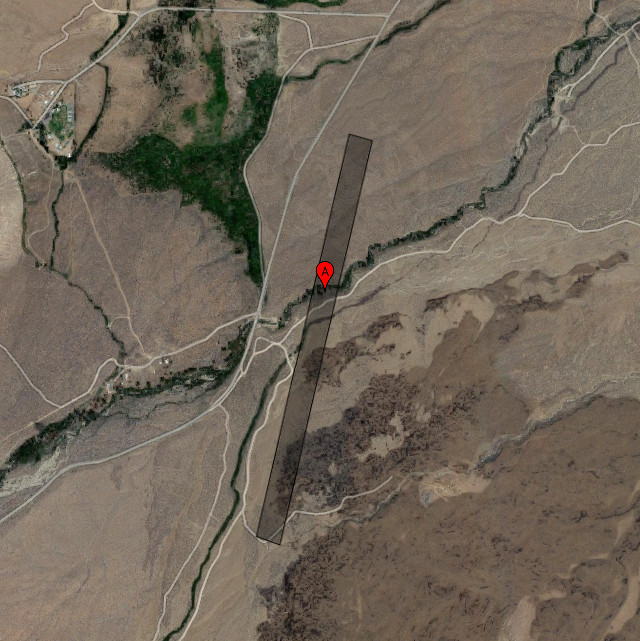
\includegraphics[width=0.45\textwidth]{figures/chapter2/google-maps-rfi-localization} &
        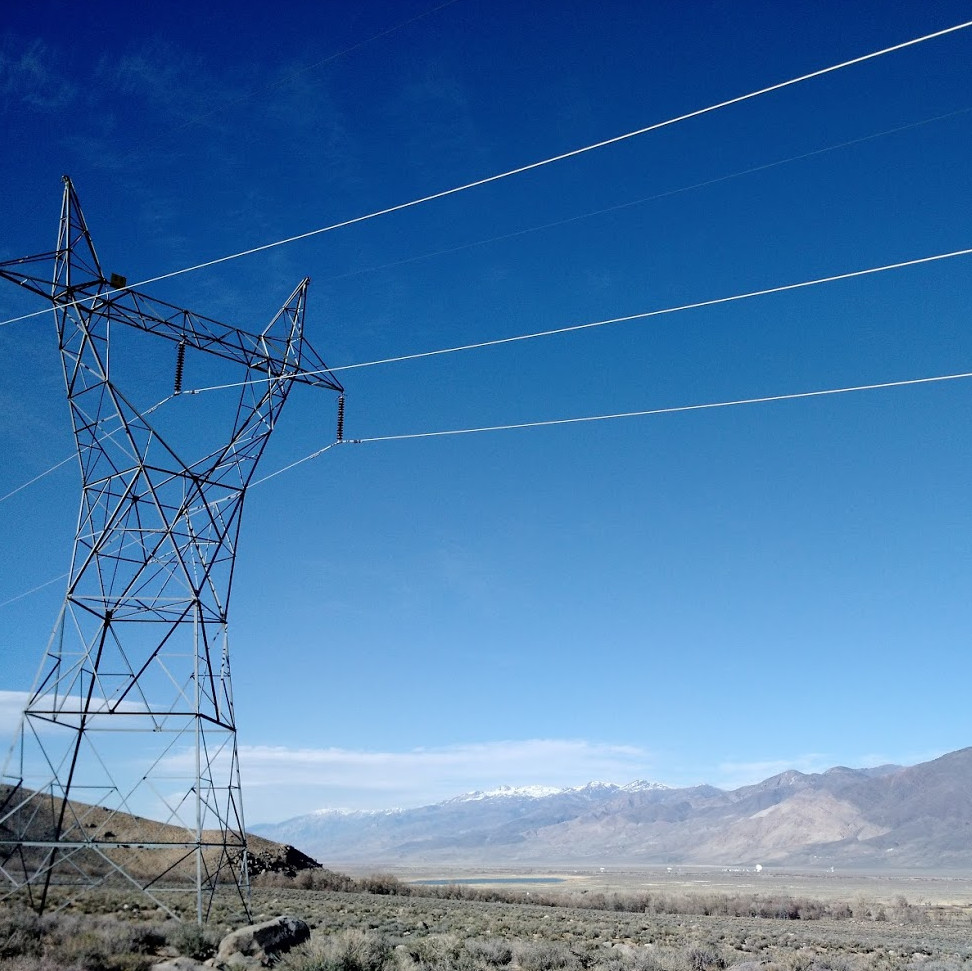
\includegraphics[width=0.45\textwidth]{figures/chapter2/power-line-picture} \\
        (a) & (b) \\
    \end{tabular}
    \caption{
        (a) The localization region (roughly 100\,m by 1.5\,km) for a source of RFI south of the
        OVRO-LWA and near the town of Big Pine. Satellite imagery \textcopyright2018 Google. Map
        data \textcopyright2018 Google.
        (b) Image of a high-voltage power line overlooking OVRO near the localization region.
    }
    \label{fig:rfi-localization}
\end{figure}

An ongoing challenge faced by the OVRO-LWA is the presence of broadband sources of radio frequency
interference (RFI) in the vicinity of the observatory. Due to the entire-hemisphere field of view of
the OVRO-LWA, these sources appear as points on the horizon that limit the sensitivity of snapshot
images through additional sidelobe noise. Further complicating matters, because this RFI originates
from the horizon, the antennas shadow each other leading to an unpredictable antenna responses in
the direction of each source. This impedes traditional deconvolution techniques.  Fortunately,
because these sources are typically in the near-field of the interferometer, the curvature of the
incoming wavefront can be used to infer the distance to each source of RFI.

The path difference from a source in the near-field of an interferometer located at the position
$(\xi, \eta, \zeta)$ to two antennas located respectively at $(x_i, y_i, z_i)$ and $(x_j, y_j, z_j)$
is
\begin{equation}\label{eq:nearfield-path-difference}
    \Delta l^\text{near-field}_{ij} =
        \sqrt{(x_j - \xi)^2 + (y_j - \eta)^2 + (z_j - \zeta)^2}
        - \sqrt{(x_i - \xi)^2 + (y_i - \eta)^2 + (z_i - \zeta)^2}\,.
\end{equation}
In the limit that the distance of the source goes to infinity, we recover the familiar expression
\begin{equation}\label{eq:farfield-path-difference}
    \Delta l^\text{far-field}_{ij} = \frac{1}{D}\Big(
        (x_i - x_j)\,\xi + (y_i - y_j)\,\eta + (z_i - z_j)\,\zeta
    \Big)\,,
\end{equation}
where $D$ is the distance to the source. The correlation measured between two antennas for a source
in the near-field of the interferometer is therefore
\begin{equation}\label{eq:nearfield-visibilities}
    V_{ij} = F \exp\Big(2\pi i \Delta l^\text{near-field}_{ij}/\lambda\Big)\,,
\end{equation}
where $V_{ij}$ is the visibility measured between antennas $i$ and $j$, $F$ is the apparent
brightness of the source, and $\lambda$ is the wavelength.

In 2016 May, I used Equation~\ref{eq:nearfield-visibilities} to estimate the position of the four
sources of RFI at 67\,MHz. The brightest of these sources can be seen in the lower-right corner of
Figure~\ref{fig:northing-easting-mistake}, and its localization can be seen in
Figure~\ref{fig:rfi-localization}. This work was instrumental in identifying faulty insulators on
high-voltage power lines as the source of pulsed broadband RFI. While this particular source of RFI
has now been repaired, we are working with the Los Angeles Department of Water and Power (LADWP) to
identify and repair the remaining RFI sources.

\subsection{Polarization Swaps}

While performing maintenance on antennas, occasionally the signal paths corresponding to the $x$ and
$y$ dipoles would be carelessly swapped.\footnote{
    The author of this thesis accepts responsibility for some---but not all---of these events!
}
After correlation, this would lead to some $xx$ and $yy$ correlations being mislabeled as $xy$ and
$yx$ correlations, and vice versa. This is clearly a problem for polarized imaging, because it
allows unpolarized emission to spill into the polarized images. Similar errors are produced in
unpolarized images, but the fractional error is less due to the fact that most of the sky emission
is unpolarized at low frequencies.

Marin Anderson identified a simple metric that allows for the rapid identification of antennas with
polarizations swapped. That is, if the amplitude for most baselines involving a given antenna have
the property that the cross-polarization visibilities are higher amplitude than the co-polarization
visibilities then it can be said with high confidence that this antenna has a polarization swap. I
built a tool that relabels the polarizations in datasets with a known set of ``swapped antennas.''

\subsection{Gain Fluctuations}

\begin{figure}
    \centering
    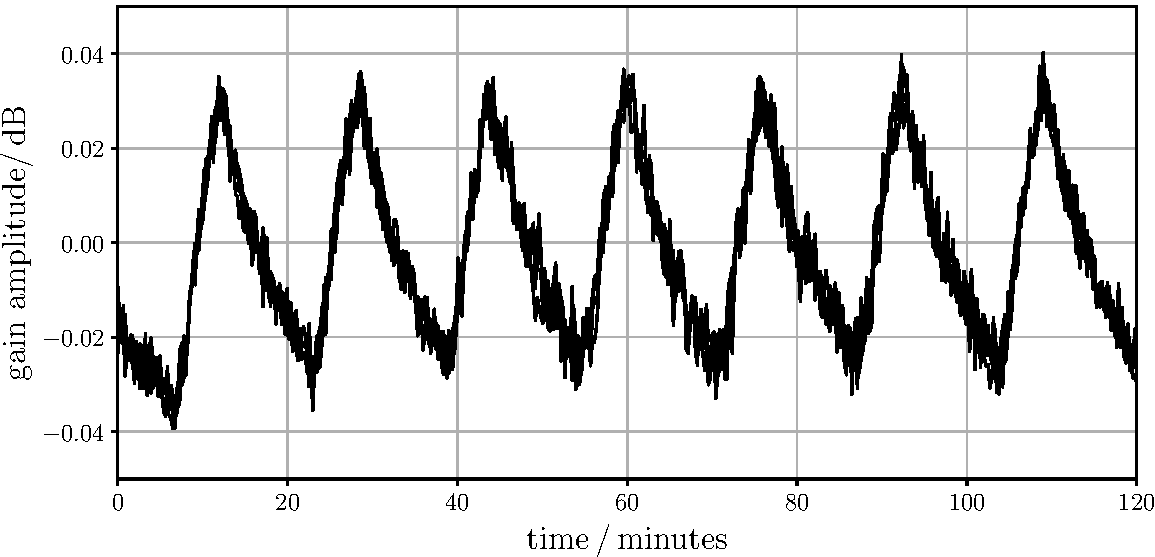
\includegraphics[width=\textwidth]{figures/chapter2/sawtooth/sawtooth}
    \caption{
        Measurement of the ``sawtooth'' fluctuations in the receiver gains associated with
        temperature variations within the electronics shelter. Four antenna traces are shown here to
        demonstrate that the gain variations are coherent between signal paths.
    }
    \label{fig:sawtooth-gains}
\end{figure}

The OVRO-LWA's receivers are located within a temperature controlled shelter. During typical
operation, the air conditioning system cycles on a 15--17\,minute timescale. The action of this is
that the temperature within shelter varies with a 15--17\,minute period. The total amplification
within the analog signal path is temperature sensitive and varies by $\sim 0.1\,\text{dB}$ within a
cycle. These gain fluctuations are illustrated in Figure~\ref{fig:sawtooth-gains}.

Typically, the complex gain calibration described in \S\ref{sec:gain-calibration} is performed once
per day, and therefore does not account for the gain fluctuations associated with these temperature
fluctuations. We add an additional stage of gain calibration to account for these time fluctuations.
The amplitude of each antenna's auto-correlation is smoothed on a 45\,minute timescale to remove the
contribution of the sawtooth pattern to each auto-correlation. The ratio of the smoothed
auto-correlations to the original auto-correlation defines a per-antenna correction that is then
applied to the cross-correlations, removing the amplitude fluctuations with respect to time. This
procedure does not account for any fluctuations in the phase with respect to time.

In principle, one could account for gain fluctuations (amplitude and phase) by recalibrating more
frequently than once per day. Ideally, one might even like to critically sample the sawtooth
fluctuations seen in Figure~\ref{fig:sawtooth-gains}. In practice, however, this is difficult due to
the availability of strong calibrator sources (if Cyg~A and Cas~A are at low elevations or below the
horizon, calibration is difficult), and the need to use $\gtrsim 10$\,minutes of data during
calibration to avoid ionospheric fluctuations impacting the gain solution. Future development of the
OVRO-LWA should record the temperature outside near the antennas, and near the analog receivers to
aid in calibrating these gain fluctuations.

\subsection{Common-Mode RFI}

With the current analog signal path of the OVRO-LWA there appears to be an additive component to the
measured visibilities (see Figure~\ref{fig:fitrfi} for images of the contribution to snapshot
images). While the impact of this apparent common-mode RFI will be discussed in more detail in
\S\ref{sec:rfi}, we will briefly summarize how this is mitigated here.

The operating principle is that terrestrial sources of RFI are not attached to the sky and therefore
do not sweep through the fringe pattern of the interferometer at the sidereal rate. Instead these
sources can be at a fixed position whether the interference enters through the antennas or somehow
couples into the analog signal path. Therefore, by simply averaging the measured correlations over a
period of 24\,hr, the contribution of true sky emission is smeared over tracks of constant
declination. Persistent sources of RFI, however, will generally add coherently.

We identify pairs of antennas that are especially susceptible to common-mode RFI by comparing the
amplitude of each correlation after averaging to other baselines of similar length. This measurement
essentially constrains the degree to which a correlation is washed out by time averaging. A
correlation that does not appear to drop in amplitude after averaging is assumed to carry a large
component due to common-mode RFI.  Antenna pairs with adjacent signal paths within the receiver tend
to register as outliers, which is suggestive of some amount of cross-coupling between the signal
paths. However, this is not a complete explanation, and physical proximity of the signal paths is
not a requirement for a correlation to be dominated by common-mode RFI.

In addition to flagging these baselines, the dominant components of the time-averaged visibilities
are taken as models for the RFI contribution to the visibilities. The model of each RFI component is
then scaled and removed from each integration to help suppress the degree of contamination. This
process is somewhat successful in removing ring-like artifacts in long synthesis images (see
Figure~\ref{fig:rings}), but ongoing development at the OVRO-LWA will see the replacement of the
analog receivers, which will obviate the need for the modeling and removal of this pickup.

\myputbib{thesis}
\end{bibunit}


\chapter{The Radio Sky at Meter Wavelengths: $m$-mode Analysis Imaging with the OVRO-LWA}

\begin{bibunit}

%%%%%%%%%%%%%%%%%%%%%%%%%%%%%%%%%%%%%%%%%%%%%%%%%%%%%%%%%%%%%%%%%%%%%%%%%%%%%%%%%%%%%%%%%%%%%%%%%%%%
\section{Introduction}

At redshifts $20 \gtrsim z \gtrsim 7$, the 21~cm hyperfine structure line of neutral hydrogen is
expected to produce a 10 to 100 mK perturbation in the cosmic microwave background (CMB) spectrum
\citep{2006PhR...433..181F, 2012RPPh...75h6901P}. The amplitude of this perturbation on a given line
of sight is a function of the neutral fraction of hydrogen, the baryon overdensity, the spin
temperature relative to the CMB temperature at the given redshift, and the line-of-sight peculiar
velocity of the gas.  The spatial power spectrum of this perturbation is thought to be dominated by
inhomogeneous heating of the intergalactic medium (IGM) at $z\sim 20$ \citep{2014MNRAS.437L..36F},
and by growing ionized bubbles during the epoch of reionization (EoR) at $z\sim 7$, where a
detection can constrain the ionizing efficiency of early galaxies, the UV photon mean-free path, and
the minimum halo mass that can support star formation \citep{2015MNRAS.449.4246G}.

Current 21~cm cosmology experiments can be broadly separated into two classes: global signal
experiments that aim to detect the spectral signature of the cosmologically redshifted 21~cm
transition after averaging over the entire sky (otherwise known as the monopole) and power spectrum
experiments that incorporate angular information to attempt to measure the 3D spatial power spectrum
of cosmological 21~cm perturbations.  Ongoing global signal experiments include EDGES
\citep{2017ApJ...847...64M}, LEDA \citep{2017arXiv170909313P}, BIGHORNS \citep{2015PASA...32....4S},
SCI-HI \citep{2014ApJ...782L...9V}, and SARAS 2 \citep{2017arXiv170306647S}.  Ongoing power spectrum
experiments include PAPER/HERA \citep{2015ApJ...809...61A, 2016arXiv160607473D}, LOFAR
\citep{2017ApJ...838...65P}, and the MWA \citep{2016ApJ...833..102B, 2016MNRAS.460.4320E}. Recently,
EDGES reported the first detection of 21~cm absorption in the globally averaged sky signal
\citep{2018Natur.555...67B}.

Just as for CMB experiments, foreground removal or suppression is an essential component of both
classes of 21~cm cosmology experiments. The brightness temperature of the galactic synchrotron
emission at high galactic latitudes is measured by \citet{2017MNRAS.464.4995M} as
\begin{equation}
    T \sim 300\,{\rm K} \times \left(\frac{\nu}{150\,{\rm MHz}}\right)^{-2.6}\,.
\end{equation}
Therefore, experiments conservatively need to achieve five orders of dynamic range against this
foreground emission before the cosmological signal can be measured. Current foreground removal
methods (for example, \citealt{2012ApJ...756..165P} and \citealt{2013MNRAS.429..165C}) rely on the
assumption that the foreground emission is spectrally smooth. The low-frequency radio sky is
composed of several components: galactic synchrotron emission, supernova remnants, radio galaxies,
free-free emission and absorption from \ion{H}{2} regions, and a confusing background of radio
sources.  Ideally, a foreground removal strategy should be informed by the measured spatial
structure and frequency spectrum of all foreground components. For instance, CMB experiments
typically construct several maps at several frequencies to enable component separation.  At low
frequencies, this possibility is limited by the availability of suitable high-fidelity sky maps on
angular scales ranging from tens of degrees to arcminutes.

Recently, a host of new low-frequency sky surveys have been conducted, including MSSS
\citep{2015A&A...582A.123H}, GLEAM \citep{2015PASA...32...25W}, and TGSS
\citep{2017A&A...598A..78I}. However, the primary data product generated by these surveys is a
catalog of radio point sources. At 45 MHz, \citet{2011A&A...525A.138G} created a map of the sky that
captures the diffuse emission with 5$^\circ$ resolution.  The LWA1 Low Frequency Sky Survey
\citep[LLFSS;][]{2017MNRAS.469.4537D} similarly maps the sky at a range of frequencies between
35 and 80~MHz with resolution between 4.5$^\circ$ and 2$^\circ$.

The Global Sky Model \citep[GSM;][]{2008MNRAS.388..247D} is currently the most commonly used
foreground model. The GSM is a nonparametric interpolation of various maps between 10 MHz and 100
GHz. However, the majority of information contained in the GSM is derived at frequencies $>1.4$~GHz,
where the majority of the modern, high-fidelity input maps are located. At 408~MHz, the venerable
Haslam map \citep{1981A&A...100..209H, 1982A&AS...47....1H} covers the entire sky at $1^\circ$
resolution.  Below 408~MHz, the GSM uses three input sky maps. \citet{2017MNRAS.464.3486Z}
constructed an improved GSM with five maps below 408~MHz, and \citet{2017MNRAS.469.4537D} used the
LWA1 to improve the GSM with their own sky maps.  However, the GSM generally suffers from low
angular resolution ($\sim 5^\circ$) and systematic errors associated with instrumental artifacts in
the input maps.  For instance, \citet{2017MNRAS.469.4537D} reported errors of $\pm 50\%$ between the
GSM and their own maps at 74 MHz, which they attribute to the increasing contribution of free-free
absorption and modifications to the synchrotron spectral index at low frequencies.

Wide-field interferometric synthesis imaging is a challenging computational problem, and it has been
particularly difficult to capture large angular scales $\gg 10^\circ$ and small angular scales $\ll
1^\circ$ in a single synthesis image. We will derive a new imaging technique -- Tikhonov-regularized
$m$-mode analysis imaging -- that allows a drift-scanning interferometer to image the entire visible
sky in a single coherent synthesis imaging step with no gridding and no mosaicking.

As a demonstration of this technique, we apply Tikhonov-regularized $m$-mode analysis imaging to the
Owens Valley Radio Observatory Long Wavelength Array (OVRO-LWA) and generate a series of new
low-frequency maps of the sky between 36.528 and 73.152~MHz.  These maps capture the full sky
visible from OVRO with an angular resolution of $\sim 15$~arcmin.  These new maps complement the
existing full-sky maps at these frequencies with greatly improved angular resolution.

We aim for these maps to inform foreground removal strategies in 21~cm cosmology, and we anticipate
additional ancillary science taking advantage of the combination of high fidelity and high
resolution of these maps, including but not limited to studies of the cosmic-ray emissivity at low
frequencies, searches for giant radio galaxies, and constraining the galactic synchrotron spectrum.
The maps will be made freely available online at the Legacy Archive for Microwave Background Data
Analysis (LAMBDA)\footnote{
    \url{https://lambda.gsfc.nasa.gov/product/foreground/fg_ovrolwa_radio_maps_info.cfm}
}.

The structure of this paper is as follows. In \S\ref{sec:imaging}, we present Tikhonov-regularized
$m$-mode analysis imaging, a new imaging technique that allows us to image the entire visible sky in
one coherent synthesis imaging step with exact wide-field corrections. In \S\ref{sec:observations}
we describe our observations with the OVRO-LWA. In \S\ref{sec:results} we present the sky maps and
compare these maps against other low-frequency sky maps.  In \S\ref{sec:error}, we discuss some of
the sources of error present in the maps, and finally, in \S\ref{sec:conclusion} we present our
conclusions.

%%%%%%%%%%%%%%%%%%%%%%%%%%%%%%%%%%%%%%%%%%%%%%%%%%%%%%%%%%%%%%%%%%%%%%%%%%%%%%%%%%%%%%%%%%%%%%%%%%%%
\section{All-sky Imaging}\label{sec:imaging}

The goal of all imaging algorithms is to estimate the brightness of the sky $I_\nu(\hat r)$ in the
direction $\hat r$ and frequency $\nu$.  A radio interferometer measures the visibilities
$V^{ij,pq}_{\nu}$ between pairs of antennas numbered $i$ and $j$ respectively, and between
polarizations labeled $p$ and $q$ respectively. We will neglect subtleties associated with polarized
imaging, so the Stokes~$I$ visibilities are constructed from the sum of the $pp$ and $qq$
correlations such that $V^{ij}_{\nu} = (V^{ij,pp}_{\nu}+V^{ij,qq}_{\nu})/2$.  If the antennas are
separated by the baseline $\vec b_{ij}$, and $A_\nu(\hat r)$ describes an antenna's response to the
incident Stokes~$I$ radiation (here assumed to be the same for each antenna), then
\begin{equation}\label{eq:basic-imaging}
    V^{ij}_\nu = \int_\text{sky}
                 A_\nu(\hat r) I_\nu(\hat r)
                 \exp\bigg(2\pi i \hat r\cdot\vec b_{ij}/\lambda\bigg) \,\d\Omega \, ,
\end{equation}
where the integral runs over the solid angle $\Omega$.  Constructing an image from the output of a
radio interferometer consists of estimating $I_\nu(\hat r)$ given the available measurements
$V^{ij}_\nu$.

For later convenience, we will define the baseline transfer function $B^{ij}_\nu(\hat r)$ such that
\begin{equation}\label{eq:baseline-transfer-function}
    V^{ij}_\nu = \int_\text{sky} B^{ij}_\nu(\hat r) I_\nu(\hat r) \,\d\Omega \, .
\end{equation}
The baseline transfer function defines the response of a single baseline to the sky and is a
function of the antenna primary beam, and baseline length and orientation.

Naively, one might attempt to solve Equation~\ref{eq:basic-imaging} by discretizing and
subsequently solving the resulting matrix equation. If the interferometer is composed of
$N_\text{base}$ baselines and measures $N_\text{freq}$ frequency channels over $N_\text{time}$
integrations, then the entire data set consists of $N_\text{base}N_\text{freq}N_\text{time}$ complex
numbers. If the sky is discretized into $N_\text{pix}$ pixels, then the relevant matrix has
dimensions of $(N_\text{base}N_\text{freq}N_\text{time})\times(N_\text{pix})$. For making
single-channel maps with the OVRO-LWA, this becomes a 5 PB array (assuming each matrix element
is a 64 bit complex floating point number).  This matrix equation is therefore prohibitively large,
and solving Equation~\ref{eq:basic-imaging} by means of discretization is usually intractable,
although \citet{2017MNRAS.465.2901Z} demonstrated this technique with the MITEOR telescope.

Instead, it is common to make mild assumptions that simplify Equation~\ref{eq:basic-imaging} and
ease the computational burden in solving for $I_\nu(\hat r)$. For example, when all of the baselines
$\vec b_{ij}$ lie in a plane and the field of view is small, Equation~\ref{eq:basic-imaging} can be
well approximated by a two-dimensional Fourier transform \citep{2001isra.book.....T}. The
restriction on baseline coplanarity and field of view can be relaxed by using W-projection
\citep{2008ISTSP...2..647C}. Known primary beam effects can also be accounted for during imaging by
using A-projection \citep{2013ApJ...770...91B}.

\subsection{$m$-mode Analysis}\label{sec:mmode-analysis}

Transit telescopes can take advantage of a symmetry in Equation~\ref{eq:basic-imaging} that greatly
reduces the amount of computer time required to image the full sky with exact incorporation of
wide-field imaging effects. This technique, called $m$-mode analysis, also obviates the need for
gridding and mosaicking. Instead, the entire sky is imaged in one coherent synthesis imaging step.
We will briefly summarize $m$-mode analysis below, but the interested reader should consult
\citet{2014ApJ...781...57S, 2015PhRvD..91h3514S} for a complete derivation.

In the context of $m$-mode analysis, a transit telescope is any interferometer for which the
response pattern of the individual elements does not change with respect to time. This may be an
interferometer like the OVRO-LWA, where the correlation elements are fixed dipoles, but it may also
be an interferometer like LOFAR or the MWA if the steerable beams are held in a fixed position (not
necessarily at zenith). The interferometer also does not necessarily have to be homogeneous.
Heterogeneous arrays composed of several different types of antennas are allowed as long as care is
taken to generalize Equation~\ref{eq:basic-imaging} for a heterogeneous array.

For a transit telescope, the visibilities $V^{ij}_\nu$ are a periodic function of sidereal
time.\footnote{
    This is not strictly true. Ionospheric fluctuations and non-sidereal sources (such as the Sun)
    will violate this assumption. This paper will, however, demonstrate that the impact on the final
    maps is mild.
}
Therefore, it is a natural operation to compute the Fourier transform of the visibilities with
respect to sidereal time $\phi\in[0,2\pi)$.
\begin{equation}
    V^{ij}_{m,\nu} = \int_0^{2\pi} V^{ij}_\nu(\phi)\exp\bigg(-im\phi\bigg)\,\d\phi
\end{equation}
The output of this Fourier transform is the set of $m$-modes $V^{ij}_{m,\nu}$ where
$m=0,\,\pm1,\,\pm2,\,\ldots$ is the Fourier conjugate variable to the sidereal time. The $m$-mode
corresponding to $m=0$ is a simple average of the visibilities over sidereal time. Similarly, $m=1$
corresponds to the component of the visibilities that varies over half-day timescales. Larger values
of $m$ correspond to components that vary on quicker timescales.

\citet{2014ApJ...781...57S, 2015PhRvD..91h3514S} showed that there is a discrete linear relationship
between the measured $m$-modes $V^{ij}_{m,\nu}$ and the spherical harmonic coefficients of the sky
brightness $a_{lm,\nu}$.
\begin{equation}\label{eq:m-mode-sum-equation}
    V^{ij}_{m,\nu} = \sum_l B^{ij}_{lm,\nu} a_{lm,\nu}\,,
\end{equation}
where the transfer coefficients $B^{ij}_{lm,\nu}$ are computed from the spherical harmonic transform
of the baseline transfer function defined by Equation~\ref{eq:baseline-transfer-function}. These
transfer coefficients define the interferometer's response to the corresponding spherical harmonic
coefficients.

Equation~\ref{eq:m-mode-sum-equation} can be recognized as a matrix equation, where the transfer
matrix $\b B$ is block-diagonal:
\begin{equation}\label{eq:m-mode-matrix-equation}
    \overbrace{\left(
        \begin{array}{c}
            \vdots \\
            m\text{-modes} \\
            \vdots \\
        \end{array}
    \right)}^{\b v}
    =
    \overbrace{\left(
        \begin{array}{ccc}
            \ddots & & \\
            & \text{transfer matrix} & \\
            & & \ddots \\
        \end{array}
    \right)}^{\b B}
    \overbrace{\left(
        \begin{array}{c}
            \vdots \\
            a_{lm} \\
            \vdots \\
        \end{array}
    \right)}^{\b a}
\end{equation}
\begin{equation}
    \b B = \left(\begin{array}{cccc}
        m = 0 &&& \\
              & m=\pm1 && \\
              && m=\pm2 & \\
              &&& \ddots \\
    \end{array}\right)
\end{equation}
The vector $\b v$ contains the list of $m$-modes and the vector $\b a$ contains the list of
spherical harmonic coefficients representing the sky brightness. In order to take advantage of the
block-diagonal structure in $\b B$, $\b v$ and $\b a$ must be sorted by the absolute value of $m$.
Positive and negative values of $m$ are grouped together because the brightness of the sky is
real-valued, and the spherical harmonic transform of a real-valued function has $a_{l(-m)} = (-1)^m
a_{lm}^*$.

In practice, we now need to pick the set of spherical harmonics we will use to represent the sky.
For an interferometer like the OVRO-LWA with many short baselines, a sensible choice is to use all
spherical harmonics with $l\le l_\text{max}$ for some $l_\text{max}$. The parameter $l_\text{max}$
is determined by the maximum baseline length of the interferometer.  For an interferometer without
short spacings, a minimum value for $l$ might also be used. This $l_\text{min}$ parameter should be
determined by the minimum baseline length. A rough estimate of $l$ for a baseline of length $b$ at
frequency $\nu$ is $l \sim \pi b\nu/c$. Based on this estimate for the OVRO-LWA and other
computational considerations, we therefore adapt $l_\text{min}=1$ and $l_\text{max}=1000$ across all
frequencies. However, this choice of $l_\text{max}$ actually limits the angular resolution above
55~MHz, and therefore future work will increase $l_\text{max}$ to obtain better angular resolution.

The interferometer's sensitivity to the monopole ($a_{00}$) deserves special consideration.
\citet{2016ApJ...826..116V} proveed -- under fairly general assumptions -- that a baseline with
nonzero sensitivity to $a_{00}$ must also have some amount of cross-talk or common-mode noise.  In
fact, the sensitivity to $a_{00}$ is proportional to a sum of these effects. For example, one way a
baseline can have nonzero sensitivity to $a_{00}$ is if the baseline is extremely short. In this
case, the antennas are so close together that voltage fluctuations in one antenna can couple into the
other antenna. In order to make an interferometric measurement of $a_{00}$, this coupling must be
measured and calibrated. Consequently, we set $a_{00}=0$ in our analysis. In the future, this
limitation will be addressed with the inclusion of calibrated total power radiometry.

The size of a typical block in the transfer matrix is
$(2N_\text{base}N_\text{freq})\times(l_\text{max})$. If each element of the matrix is stored as a
64 bit complex floating point number, a single block is 500 MB for the case of single-channel
imaging with the OVRO-LWA, which a modern computer can easily store and manipulate in memory.
However, with additional bandwidth, these blocks quickly become unwieldy; thus, as a first pass, the
analysis in this paper is restricted to single-channel imaging. Note also that for the OVRO-LWA,
$N_\text{base} \gg l_\text{max}$, so there are more measurements than unknowns in
Equation~\ref{eq:m-mode-matrix-equation}.

The key advantage of $m$-mode analysis is the block-diagonal structure of
Equation~\ref{eq:m-mode-matrix-equation}. The computational complexity of many common matrix
operations (e.g., solving a linear system of equations) is $\mathcal{O}(N^3)$, where $N$ is the
linear size of the matrix.  By splitting the equation into $M$ independent blocks, the number of
floating point operations required to solve the linear system of equations is now
$\mathcal{O}(N^3M^{-2})$, because each block can be manipulated independently of the other blocks.
This computational savings is what makes this matrix algebra approach to interferometric imaging
feasible. For the data set presented in this paper, computing the elements of the transfer matrix
takes $\sim$10 hours per frequency channel on a 10-node cluster, but once the matrix has been
computed, the imaging process described in \S\ref{sec:mmode-imaging} takes $\sim$10 minutes, and the
deconvolution process described in \S\ref{sec:clean} was allowed to run for $\sim$10 hours.

\subsection{$m$-mode Analysis Imaging}\label{sec:mmode-imaging}

Imaging in $m$-mode analysis essentially amounts to inverting
Equation~\ref{eq:m-mode-matrix-equation} to solve for the spherical harmonic coefficients $\b a$.
The linear least-squares solution, which minimizes $\|\b v - \b B\b a\|^2$, is given by
\begin{equation}
    \b{\hat a}_\text{LLS} = (\b B^*\b B)^{-1}\b B^*\b v\,,
\end{equation}
where $^*$ indicates the conjugate-transpose.

However, usually one will find that $\b B$ is not full rank, and hence $\b B^*\b B$ is not an
invertible matrix. For example, an interferometer located in the northern hemisphere will never see
a region of the southern sky centered on the southern celestial pole. The $m$-modes contained in the
vector $\b v$ must contain no information about the sky around the southern celestial pole, and
therefore the act of multiplying by $\b B$ must destroy some information about the sky. The
consequence of this fact is that $\b B$ must have at least one singular value that is equal to zero.
It then follows that $\b B^*\b B$ must have at least one eigenvalue that is equal to zero, which
means it is not an invertible matrix.

Another way of looking at the problem is that because the interferometer is not sensitive to part of
the southern hemisphere, there are infinitely many possible solutions to
Equation~\ref{eq:m-mode-matrix-equation} that will fit the measured data equally well.  We will
therefore regularize the problem and apply an additional constraint that prefers a unique yet
physically reasonable solution.

\subsubsection{Tikhonov Regularization}

The process of Tikhonov regularization minimizes $\|\b v - \b B\b a\|^2 + \varepsilon\|\b a\|^2$ for
some arbitrary value of $\varepsilon > 0$ chosen by the observer. The solution that minimizes this
expression is given by
\begin{equation}\label{eq:tikhonov-solution}
    \b{\hat a}_\text{Tikhonov} = (\b B^*\b B + \varepsilon\b I)^{-1}\b B^*\b v\,.
\end{equation}
Tikhonov regularization adds a small value $\varepsilon$ to the diagonal of $\b B^*\b B$, fixing the
matrix's singularity. By using the singular value decomposition (SVD) of the matrix $\b B = \b U \b
\Sigma \b V^*$, Equation~\ref{eq:tikhonov-solution} becomes
\begin{equation}
    \b{\hat a}_\text{Tikhonov} = \b V (\b\Sigma^2 + \varepsilon \b I)^{-1}\b\Sigma \b U^*\b v\,,
\end{equation}
where
\[
    \b\Sigma = \left(
        \begin{array}{ccc}
            \sigma_1 & & \\
                     & \sigma_2 & \\
                     & & \ddots \\
        \end{array}
    \right)\,.
\]
The diagonal elements of $\b\Sigma$ are the singular values of $\b B$. The contribution of each
singular component to the Tikhonov-regularized solution is scaled by $\sigma_i / (\sigma_i^2 +
\varepsilon)$, where $\sigma_i$ is the singular value for the $i$th singular component. Tikhonov
regularization therefore acts to suppress any component for which
$\sigma_i\lesssim\sqrt{\varepsilon}$.  If $\sigma_i = 0$, the component is set to zero.

In practice, the measurement $\b v$ is corrupted by noise with covariance $\b N$. For illustrative
purposes, we will assume that $\b N=n\b I$ for some $n>0$. In this case, the covariance of the
Tikhonov-regularized spherical harmonic coefficients is
\begin{equation}
    \b C = n \b V (\b\Sigma^2 + \varepsilon\b I)^{-2} \b\Sigma^2 \b V^*\,.
\end{equation}
Each singular component is scaled by a factor of $\sigma_i^2/(\sigma_i^2 + \varepsilon)^2$.  In the
absence of Tikhonov regularization ($\varepsilon=0$), singular components with the smallest singular
values -- the ones that the interferometer is the least sensitive to -- actually come to dominate
the covariance of the measured spherical harmonic coefficients. Tikhonov regularization improves
this situation by down-weighting these components.

\subsubsection{L Curves}

\begin{figure}[t]
    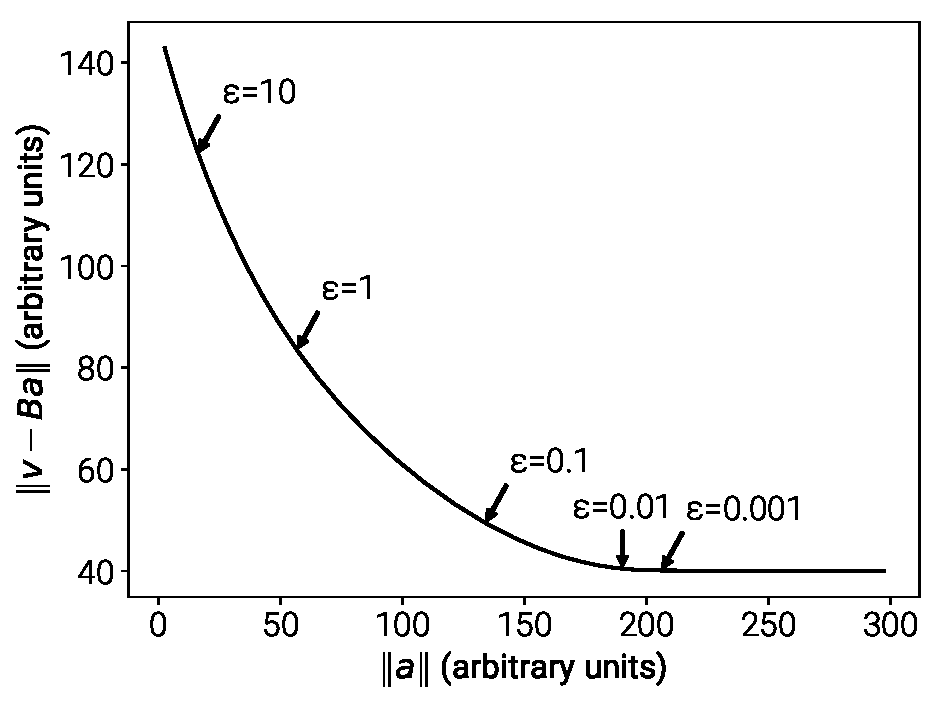
\includegraphics[width=\columnwidth]{figures/chapter3/lcurve}
    \caption{
        Example L curve computed from OVRO-LWA data at 36.528~MHz by trialing 200 different values
        of the regularization parameter $\varepsilon$. The $x$-axis is the norm of the solution (in
        this case, the spherical harmonic coefficients) given in arbitrary units, and the $y$-axis
        is the least-squares norm given in arbitrary units. Where the regularization parameter is
        small, the norm of the solution grows rapidly. Where the regularization parameter is large,
        the least-squares norm grows rapidly.
    }
    \label{fig:lcurve}
\end{figure}

Tikhonov regularization requires the observer to pick the value of $\varepsilon$. If $\varepsilon$
is too large, then too much importance is placed on minimizing the norm of the solution and the
least-squares residuals will suffer. Conversely, if $\varepsilon$ is too small, then the problem
will be poorly regularized and the resulting sky map may not represent the true sky. Picking the
value of $\varepsilon$ therefore requires understanding the trade-off between the two norms.

This trade-off can be analyzed quantitatively by trialing several values of $\varepsilon$, and
computing $\|\b v - \b B\b a\|^2$ and $\|\b a\|^2$ for each trial. An example is shown in
Figure~\ref{fig:lcurve}. The shape of this curve has a characteristic L shape, and as a result, this
type of plot is called an L curve. The ideal value of $\varepsilon$ lies near the turning point, of
the plot. At this point a small decrease in $\varepsilon$ will lead to an undesired rapid increase
in $\|\b a\|^2$, and a small increase in $\varepsilon$ will lead to an undesired rapid increase in
$\|\b v - \b B\b a\|^2$.

In practice, the L curve should be used as a guide to estimate a reasonable value of $\varepsilon$.
However, better results can often be obtained by tuning the value of $\varepsilon$. For instance,
increasing the value of $\varepsilon$ can improve the noise properties of the map by down-weighting
noisy modes. Decreasing the value of $\varepsilon$ can improve the resolution of the map by
up-weighting the contribution of longer baselines, which are likely fewer in number. In this
respect, choosing the value of $\varepsilon$ is analogous to picking the weighting scheme in
traditional imaging where robust weighting schemes can be tuned to similar effect \citep{briggs}.
For the OVRO-LWA, we selected $\varepsilon = 0.01$ across all frequency channels. The distribution
of singular values of the transfer matrix with respect to $\sqrt{\varepsilon}$ is summarized in
Table~\ref{tab:summary}.

\subsubsection{Other Regularization Schemes}

The choice of applying Tikhonov regularization to $m$-mode analysis imaging is not unique. There
exists a plethora of alternative regularization schemes that could also be applied. Each
regularization scheme has its own advantages and disadvantages. For instance, Tikhonov
regularization is simple, independent of prior information, and sets unmeasured modes to zero (a
sensible expectation). We will now briefly discuss a few other alternatives.

The Moore--Penrose pseudo-inverse (denoted with a superscript $\dagger$) is commonly applied to find
the minimum-norm linear least-squares solution to a set of linear equations. This can be used in
place of Tikhonov regularization as
\begin{equation}
    \b{\hat a}_\text{Moore-Penrose} = \b B^\dagger\b v\,.
\end{equation}
Much like Tikhonov regularization, the Moore--Penrose pseudo-inverse sets components with small
singular values (below some user-defined threshold) to zero. Components with large singular values
(above the user-defined threshold) are included in the calculation at their full amplitude with no
down-weighting of modes near the threshold. The essential difference between using the
Moore--Penrose pseudo-inverse and Tikhonov regularization is that the pseudo-inverse defines a hard
transition from ``on'' to ``off.'' Modes are either set to zero or included in the map at their full
amplitude. On the other hand, Tikhonov regularization smoothly interpolates between these behaviors.
Because of this, Tikhonov regularization tends to produce better results in practical applications.

If the measured $m$-modes have a noise covariance matrix $\b N \neq n\b I$ for some scalar $n$
(e.g., the interferometer is inhomogeneous), then the observer should minimize $(\b v-\b B\b a)^*\b
N^{-1}(\b v-\b B\b a) + \varepsilon\|\b a\|^2$. The noise covariance matrix $\b N$ is used to weight
the measurements such that
\begin{equation}
    \b{\hat a}_\text{min variance} = (\b B^*\b N^{-1}\b B + \varepsilon\b I)^{-1}
        \b B\b N^{-1}\b v\,.
\end{equation}

In the event that the observer has a prior map of the sky, $\|\b a - \b a_\text{prior}\|^2$ can be
used as the regularizing norm. This will use the prior map to fill in missing information instead of
setting these modes to zero. In this case, the minimum is at
\begin{equation}
    \b{\hat a}_\text{with prior} = (\b B^*\b B + \varepsilon\b I)^{-1}
        (\b B^*(\b v - \b B\b a_\text{prior}))
        + \b a_\text{prior}\,.
\end{equation}
If instead the observer has a prior expectation on the covariance of the spherical harmonic
coefficients, Wiener filtering can also be used.  This technique is demonstrated for simulated
measurements by \citet{2016arXiv161203255B}.

Alternatively, we could opt to regularize the problem by enforcing smoothness in the sky maps. In
this case, the regularizing norm should be of the form $\|\nabla I(\hat r)\|^2$, where $\nabla I$ is
the gradient of the sky brightness in the direction $\hat r$. This is actually a generalization of
Tikhonov regularization, where the objective function is $\|\b v-\b B\b a\|^2 + \varepsilon\|\b A\b
a\|^2$ for some matrix $\b A$. The minimum is at
\begin{equation}
    \b{\hat a}_\text{generalized} = (\b B^*\b B + \varepsilon\b A^*\b A)^{-1}\b B^*\b v\,.
\end{equation}

Finally, in many machine-learning applications the $L_1$-norm\footnote{
    $\|\b a\|_1 = \sum_i |a_i|$
} is used in place of the usual $L_2$-norm in order to encourage sparsity in the reconstructed
signal. Applying this to $m$-mode analysis imaging would amount to minimizing $\|\b v-\b B\b a\|_2^2
+ \varepsilon\|\b a\|_1$. However, because we have decomposed the sky in terms of spherical
harmonics, the vector $\b a$ is not expected to be sparse. Consequently, the $L_1$-norm is generally
inappropriate for $m$-mode analysis imaging without an additional change of variables designed to
introduce sparsity.

\subsection{CLEAN}\label{sec:clean}

In traditional radio astronomy imaging, CLEAN \citep{1974A&AS...15..417H} is a physically motivated
algorithm that interpolates between measured visibilities on the $uv$ plane. In the absence of this
interpolation, gaps in the interferometer's $uv$ coverage are assumed to be zero, and -- in the
image plane -- sources are convolved with a point spread function (PSF) that is characteristic of
the $uv$ coverage.  Fundamentally, the interferometer's PSF is determined by which modes were
assumed to be zero in the initial imaging process.

In $m$-mode analysis imaging, we assumed modes were zero in two separate ways.
\begin{enumerate}
    \item We selected a set of spherical harmonic coefficients $a_{lm}$ to describe the
        sky-brightness distribution. All modes with $l>l_\text{max}$ are neglected and assumed to be
        zero.
    \item Tikhonov regularization forces linear combinations of spherical harmonic coefficients with
        $\sigma_i \lesssim \sqrt{\varepsilon}$ toward zero.
\end{enumerate}
As a consequence, the final map of the sky is not assembled from a complete set of spherical
harmonics. Therefore, just as in traditional imaging, $m$-mode analysis imaging produces dirty maps
in which sources are convolved with a PSF.  This PSF can be improved by increasing the number and
variety of baselines, which increases the number of modes for which $\sigma_i \gg
\sqrt{\varepsilon}$.  Alternatively, by collecting more data, the signal-to-noise ratio of the
measured $m$-modes increases, which allows the observer to lower the value of $\varepsilon$ without
increasing the noise in the maps.  Finally, the CLEAN algorithm can be applied to interpolate some
of the missing information that was assumed to be zero.

The PSF of a dirty $m$-mode analysis map may be computed with
\begin{equation}\label{eq:psf}
    \b a_\text{PSF}(\theta, \phi)
        = (\b B^*\b B + \varepsilon\b I)^{-1}\b B^*\b B\b a_\text{PS}(\theta, \phi)\,,
\end{equation}
where $\b a_\text{PSF}(\theta, \phi)$ is the vector of spherical harmonic coefficients representing
the PSF at the spherical coordinates $(\theta, \phi)$, and $\b a_\text{PS}(\theta, \phi)$ is the
vector of spherical harmonic coefficients for a point source at $(\theta, \phi)$ given by
\begin{equation}
    \b a_\text{PS}(\theta, \phi) = \begin{pmatrix}
        \vdots \\
        Y_{lm}^*(\theta, \phi) \\
        \vdots \\
    \end{pmatrix}
    = \begin{pmatrix}
        \vdots \\
        Y_{lm}^*(\theta, 0)\times e^{im\phi} \\
        \vdots \\
    \end{pmatrix} \,.
\end{equation}
In general, the PSF can be a function of the right ascension and declination. However, point sources
at the same declination take the same track through the sky and (barring any ionospheric effects)
will have the same PSF. The PSF is therefore only a function of the declination. For example,
sources at low elevations will tend to have an extended PSF along the north--south axis due to
baseline foreshortening. For the OVRO-LWA antenna configuration (Figure~\ref{fig:antenna-layout}),
example PSFs at three separate frequencies are shown in Figure~\ref{fig:psf}.  Adapting CLEAN for
$m$-mode analysis requires either precomputing Equation~\ref{eq:psf} at a grid of declinations, or
a method for rapidly evaluating Equation~\ref{eq:psf} on the fly.

For an interferometer with more baselines than spherical harmonics used in the maps (e.g., the
OVRO-LWA), $\b B^*\b B$ can be a much smaller matrix than the full transfer matrix $\b B$.
Therefore, precomputing $\b B^*\b B$ can allow the entire matrix to fit into memory on a single
machine. This greatly reduces the amount of disk I/O necessary for solving Equation~\ref{eq:psf}.

Additionally, we can precompute the Cholesky decomposition of $\b B^*\b B + \varepsilon\b I = \b
U^*\b U$, where $\b U$ is an upper triangular matrix. Inverting an upper triangular matrix is an
$\mathcal{O}(N^2)$ operation (instead of $\mathcal{O}(N^3)$ for a general matrix inverse).\footnote{
    Instead of computing $\b A^{-1}$, we solve the linear equation $\b A\b x = \b b$ each time the
    matrix inverse is needed so as to avoid numerical instabilities.
}
Equation~\ref{eq:psf} can then be rapidly evaluated from right to left as
\begin{equation}\label{eq:rapid-psf}
    \b a_\text{PSF} =
        \b U^{-1}\,\big(\b U^*\big)^{-1}\,\big(\b B^*\b B\big)\,\b a_\text{PS}\,.
\end{equation}
Furthermore, Equation~\ref{eq:rapid-psf} does not need to be separately evaluated for each CLEAN
component. Instead, we can identify $N$ CLEAN components, accumulate $\b a_\text{PS}$ for each
component, and evaluate Equation~\ref{eq:rapid-psf} on the accumulation. This can greatly reduce the
number of times this equation needs to be evaluated, but care must be taken to ensure that the $N$
components are not so close together that sidelobes from one may interact with another.

Altogether, the adaptation of CLEAN applied to the maps presented in this paper is summarized below.
\begin{algorithmic}[1]
    \Require{$\b a$ is the solution to Equation~\ref{eq:tikhonov-solution}}
    \Function{CLEAN}{$\b a$}
    \Let{$\b M$}{$\b B^*\b B$}
    \Let{$\b U$}{${\rm chol}(\b M + \varepsilon\b I)$} \Comment{Cholesky decomposition}
    \While{noise in map $>$ threshold}
    \State find $N$ pixels with the largest residual flux
    \Let{$\b x$}{$\sum_{i=1}^N \,(\text{pixel flux}) \times \b a_\text{PS}(\theta_i, \phi_i)$}
    \Let{$\b y$}{$\b U^{-1}\big(\b U^*\big)^{-1}\b M\b x$}
    \Let{$\b a$}{$\b a - (\text{loop gain})\times\b y$}
    \State record subtracted components
    \EndWhile
    \Let{$\b a$}{$\b a + (\text{restored components})$}
    \State \Return{$\b a$}
    \EndFunction
\end{algorithmic}

In summary, Tikhonov-regularized $m$-mode analysis imaging constructs a wide-field synthesis image of
the sky from a complete Earth rotation, and  with exact treatment of wide-field effects. This is
accomplished by solving a regularized block-diagonal matrix equation
(Equation~\ref{eq:tikhonov-solution}). The solution to this equation generates a map where
sources are convolved with a PSF characteristic of the interferometer (a function of the frequency,
antenna response, and baseline distribution with a full Earth rotation). The CLEAN algorithm is
adopted to deconvolve the PSF and produce the final sky maps.

%%%%%%%%%%%%%%%%%%%%%%%%%%%%%%%%%%%%%%%%%%%%%%%%%%%%%%%%%%%%%%%%%%%%%%%%%%%%%%%%%%%%%%%%%%%%%%%%%%%%
\section{Observations}\label{sec:observations}

\subsection{The OVRO-LWA}

\begin{figure}[t]
    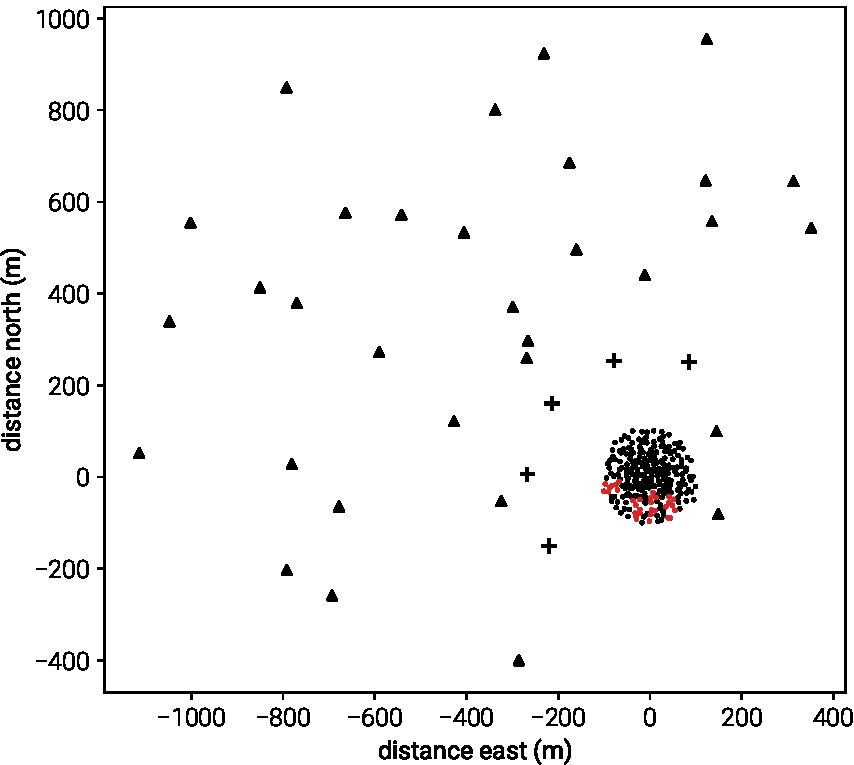
\includegraphics[width=\columnwidth]{figures/chapter3/antenna-layout}
    \caption{
        Antenna layout for the OVRO-LWA. Black dots correspond to antennas within the 200 m diameter
        core of the array. The 32 triangles are the expansion antennas built in early 2016 in order
        to increase the longest baseline to $\sim1.5$ km. The red dots are core antennas that are
        disconnected from the correlator in order to accommodate these antennas. The five crosses
        are antennas equipped with noise-switched front ends.
    }
    \label{fig:antenna-layout}
\end{figure}

\begin{figure*}[t]
    \begin{tabular}{c}
        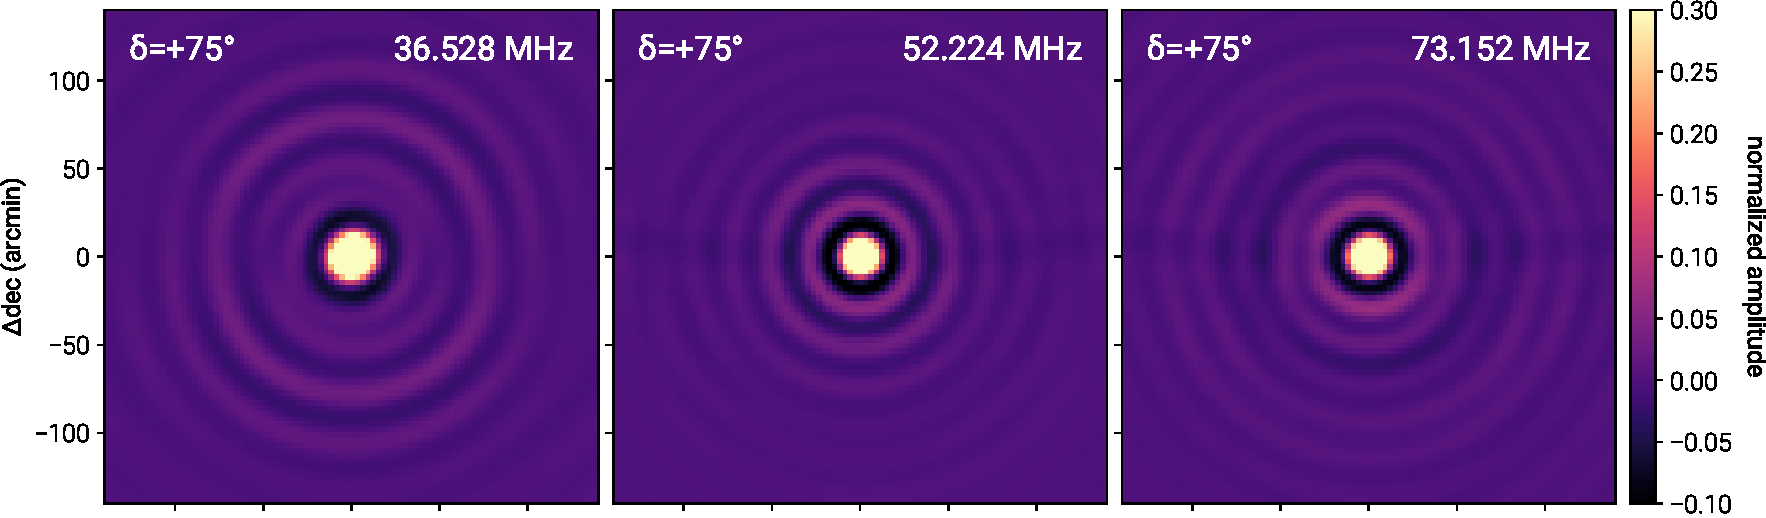
\includegraphics[width=\textwidth]{figures/chapter3/psf+75} \\
        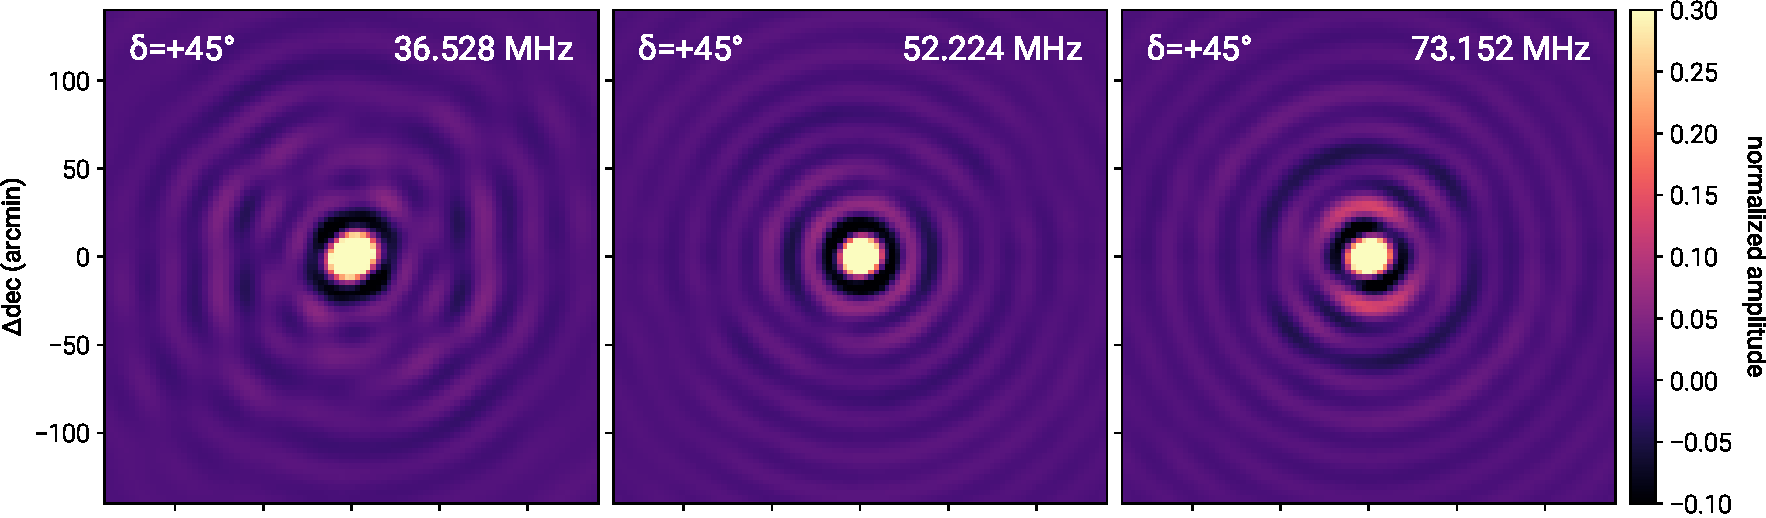
\includegraphics[width=\textwidth]{figures/chapter3/psf+45} \\
        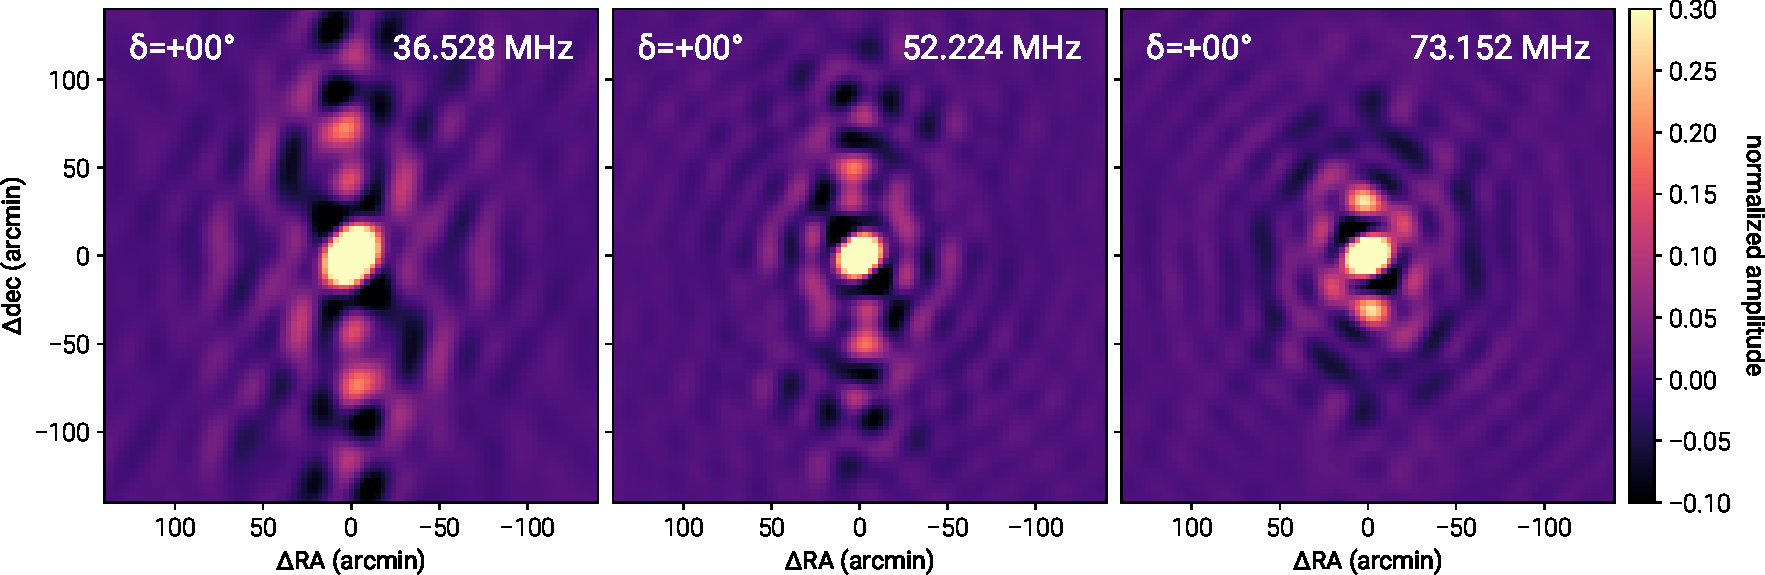
\includegraphics[width=\textwidth]{figures/chapter3/psf+0} \\
    \end{tabular}
    \caption{
        The $m$-mode analysis imaging PSF at three declinations (top row: $\delta=+75^\circ$, middle
        row: $\delta=+45^\circ$, bottom row: $\delta=+0^\circ$) and three frequencies (left column:
        36.528~MHz, middle column: 52.224~MHz, right column: 73.152~MHz).  The PSF is computed by
        evaluating Equation~\ref{eq:psf}. Above 55~MHz, the angular extent of the PSF does not
        follow the expected scaling with frequency because the angular resolution is limited by the
        selection of $l_\text{max}=1000$. The FWHM at $\delta=+45^\circ$ is listed in
        Table~\ref{tab:summary}.
    }
    \label{fig:psf}
\end{figure*}

The OVRO-LWA is a 288-element interferometer located at OVRO near Big Pine, California
\citep{hallinan_2017}.  The OVRO-LWA is a low-frequency instrument with instantaneous bandwidth
covering 27 to 85~MHz and with 24~kHz channelization.  Each antenna stand hosts two perpendicular
broadband dipoles so that there are $288\times2$ signal paths in total. These signal paths feed into
the 512-input LEDA correlator \citep{2015JAI.....450003K}, which allows the OVRO-LWA to capture the
entire visible hemisphere in a single snapshot image.

The 288 antennas are arranged in a pseudo-random configuration optimized to minimize sidelobes in
snapshot imaging (see Figure~\ref{fig:antenna-layout}).  Of these 288 antennas, 251~are contained
within a 200~m diameter core, 32~are placed outside of the core in order to extend the maximum
baseline length to $\sim$1.5~km, and five are equipped with noise-switched front ends for calibrated
total power measurements of the global sky brightness.  These antennas are used as part of the LEDA
experiment \citep{2017arXiv170909313P} to measure the global signal of 21~cm absorption from the
cosmic dawn. In the current configuration, 32 antennas (64 signal paths) from the core are
disconnected from the correlator in order to accommodate the 32 antennas on longer baselines. A
final stage of construction will involve 64 additional antennas installed on long baselines out to a
maximum length of 2.6~km.

The data set used in this paper spans 28 consecutive hours beginning at 2017 February 17 12:00:00 UTC
time.  During this time, the OVRO-LWA operated as a zenith-pointing drift-scanning interferometer.
The correlator dump time was selected to be 13~s such that the correlator output evenly divides a
sidereal day. Due to the computational considerations presented in \S\ref{sec:mmode-analysis}, eight
24~kHz channels are selected for imaging from this data set: 36.528, 41.760, 46.992, 52.224, 57.456,
62.688, 67.920, and 73.152~MHz.  These particular channels are chosen due to their location at the
exact center of instrumental subbands.

\subsection{Complex Gain Calibration}\label{sec:gaincal}

The complex gain calibration is responsible for correcting per-antenna amplitude and phase errors.
This is accomplished using a sky model and a variant of alternating least-squares colloquially known
as ``Stefcal''
\citep{2008ISTSP...2..707M, 2014A&A...571A..97S}\footnote{
    The calibration routine is written in the Julia programming language
    \citep{doi:10.1137/141000671}, and is publicly available online
    (\url{https://github.com/mweastwood/TTCal.jl}) under an open source license (GPLv3 or any later
    version).
}.

Cyg~A and Cas~A are -- by an order of magnitude -- the brightest point-like radio sources in the
northern hemisphere at resolutions lower than 0.25$^\circ$. Therefore, the optimal time to solve for
the interferometer's gain calibration is when these sources are at high elevations.  The antenna
complex gains are measured from a 22~minute track of data when Cyg~A and Cas~A are at high
elevations. The gains measured in this way are then used to calibrate the entire 28 hour data set.
The calibration sky model consists only of Cyg~A and Cas~A. The model flux of Cyg~A is set to the
\citet{1977A&A....61...99B} spectrum, while the flux of Cas~A is measured from the data itself (using
a preliminary calibration solved for with a fiducial Cas~A spectrum).

Calibrating in this manner generates approximately arcminute errors in the astrometry of the final
sky maps due to ionospheric refractive offsets during the time of calibration.  These residual
errors in the astrometry are corrected post-imaging by registering the images with respect to all
Very Large Array Low-frequency Sky Survey Redux (VLSSr) \citep{2014MNRAS.440..327L} sources that are
bright ($>30$~Jy with a consistent flux density measured with the OVRO-LWA) and not too close to
other bright sources (at least $1^\circ$ separation).

Temperature fluctuations of the analog electronics generate 0.1~dB sawtooth oscillations in the
analog gain. These oscillations occur with a variable 15 to 17~minute period associated with HVAC
cooling cycles within the electronics shelter that houses these electronics.  The amplitude of these
gain fluctuations is calibrated by smoothing the autocorrelation amplitudes on 45~minute timescales.
The ratio of the measured autocorrelation power to the smoothed autocorrelation power defines a
per-antenna amplitude correction that is then applied to the cross-correlations.  Additionally, the
ambient temperature at the front-end electronics (located in a box at the top of each dipole)
fluctuates diurnally, which will generate diurnal gain fluctuations. At this time, no correction is
made for these diurnal gain fluctuations.

\subsection{Primary Beam Measurements}\label{sec:beam}

\begin{figure*}[t]
    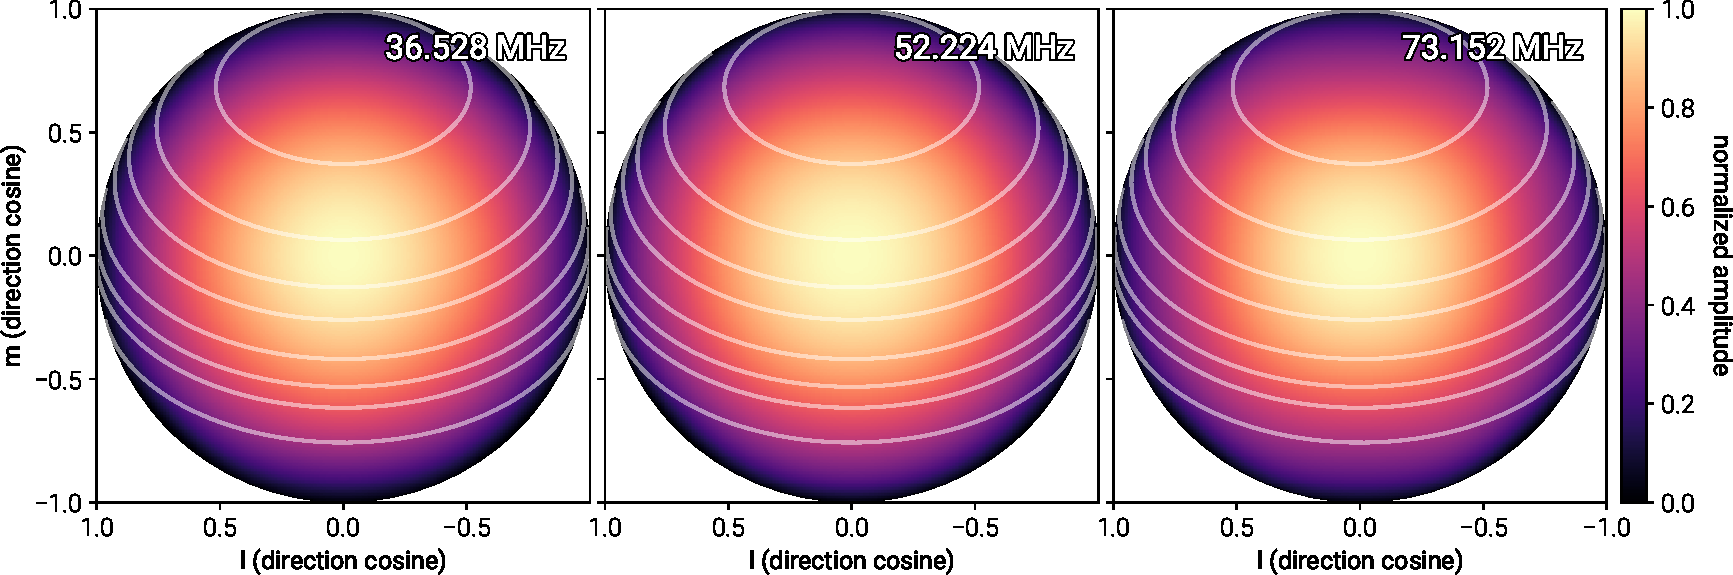
\includegraphics[width=\textwidth]{figures/chapter3/beam}
    \caption{
        Empirical fits to the OVRO-LWA Stokes $I$ primary beam (the response of the $x$ and
        $y$ dipoles has been summed) at three frequencies: 36.528 MHz (left panel), 52.224 MHz
        (middle panel), and 73.152 MHz (right panel). The source tracks used to measure the beam
        model are overlaid. From north to south, these tracks correspond to Cas~A, Cyg~A, 3C~123,
        Tau~A, Vir~A, Her~A, 3C~353, and Hya~A.  The fitting process is described in
        \S\ref{sec:beam}, and residuals for Cyg~A and Cas~A are in Figure~\ref{fig:scintillation}.
    }
    \label{fig:beam}
\end{figure*}

In order to generate wide-field images of the sky, the response of the antenna to the sky must be
known. Drift-scanning interferometers like the OVRO-LWA can empirically measure their primary beam
under a mild set of symmetry assumptions \citep{2012AJ....143...53P}. The symmetry assumptions are
necessary to break the degeneracy between source flux and beam amplitude when the flux of the source
is unknown. In this work, we assume symmetries that are apparent in the antenna design, but
real-world defects and coupling with nearby antennas will contribute toward breaking these
symmetries at some level. In particular, we assume that the $x$ and $y$ dipoles have the same
response to the sky after rotating one by $90^\circ$, and that the beam is invariant under
north--south and east--west flips.

We measure the flux of several bright sources (Cyg~A, Cas~A, Tau~A, Vir~A, Her~A, Hya~A, 3C~123, and
3C~353) as they pass through the sky and then fit a beam model composed of Zernike polynomials to
those flux measurements. We select the basis functions to have the desired symmetry ($Z_0^0$,
$Z_2^0$, $Z_4^0$, $Z_4^4$, $Z_6^0$, $Z_6^4$, $Z_8^0$, $Z_8^4$, and $Z_8^8$), and the beam amplitude
at zenith is constrained to be unity. See Figure~\ref{fig:beam} for an illustration of a fitted beam
model at several frequencies. This process is repeated for each frequency channel. Residuals for
Cyg~A and Cas~A can be seen in Figure~\ref{fig:scintillation}.

\subsection{Ionospheric Conditions}\label{sec:ionosphere-conditions}

\begin{figure*}[t]
    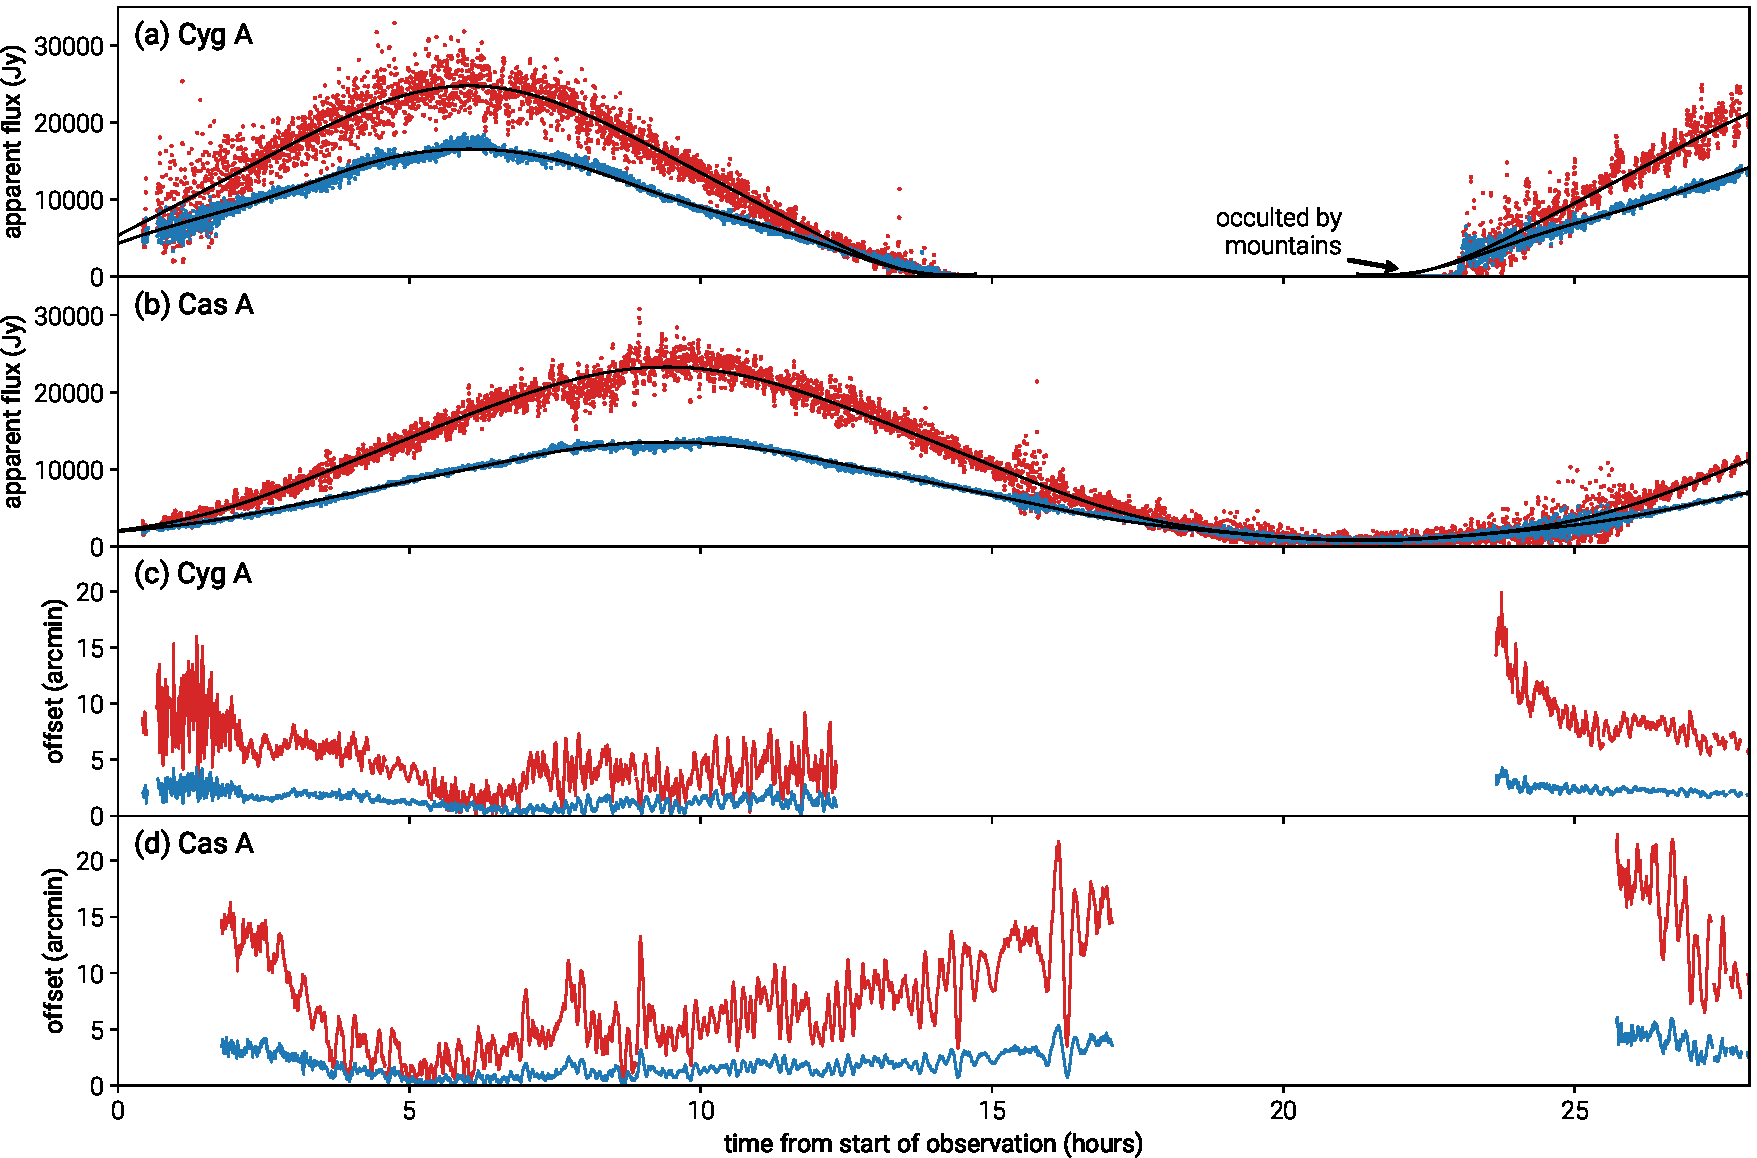
\includegraphics[width=\textwidth]{figures/chapter3/scintillation-refraction}
    \caption{
        Panels (a) and (b) show the measured apparent flux of Cyg~A and Cas~A at 36.528 MHz (red
        points) and 73.152 MHz (blue points) as a function of time over the observing period. The
        solid black curves show the expected flux computed using the empirical beam model fits. The
        thermal noise contribution to each point is about 50 Jy.  Cyg~A is occulted by the White
        Mountains when it is low on the horizon to the east.
        Panels (c) and (d) show the measured position offset of Cyg~A and Cas~A relative to their
        true astronomical positions at 36.528 MHz (red line) and 73.152 MHz (blue line).
    }
    \label{fig:scintillation}
\end{figure*}

\begin{figure}[t]
    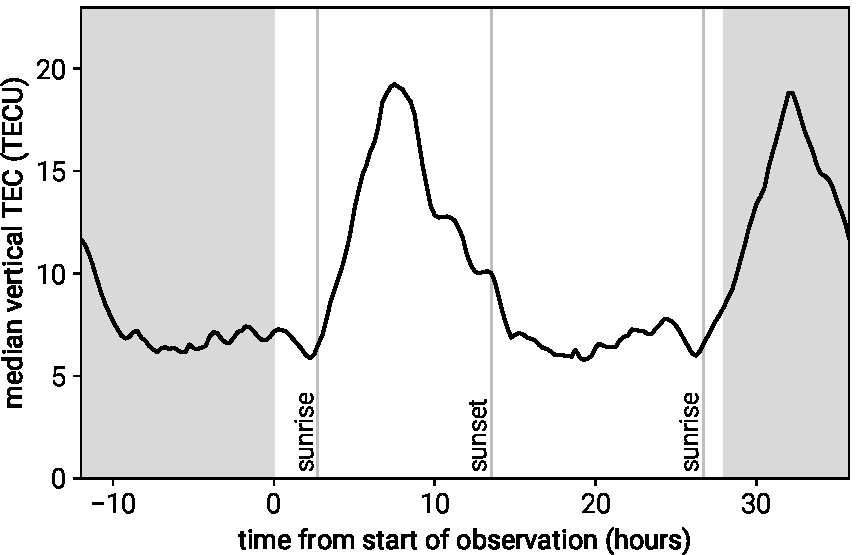
\includegraphics[width=\columnwidth]{figures/chapter3/vtec}
    \caption{
        Median vertical TEC within 200 km of OVRO during the time of the observation. The gray
        shaded regions indicate times outside of the observing period. The gray vertical lines
        indicate sunrise and sunset (as labeled).
    }
    \label{fig:vtec}
\end{figure}

The geomagnetic conditions during this time were mild. The Disturbance storm time (Dst) index, which
measures the $z$-component of the interplanetary magnetic field, was
$>-30$ nT during the entirety of the observing period.\footnote{
    The Dst index was obtained from the World Data Center for Geomagnetism, Kyoto University
    (\url{http://swdcwww.kugi.kyoto-u.ac.jp/}). Accessed 2017 July 25.
}
Following the classification scheme of \citet{2008GMS...181.....K}, a weak geomagnetic storm has
$\text{Dst} < -30$ nT. Stronger geomagnetic storms have $\text{Dst} < -50$ nT.

Despite the mild conditions, low-frequency interferometric observations are still affected by the
index of refraction in the ionosphere.  Figure~\ref{fig:vtec} shows the median vertical total
electron content (TEC) above OVRO measured from GPS \citep{1999JASTP..61.1205I}. The median is
computed over all GPS measurements within 200 km of the observatory. Over the observing period, the
TEC smoothly varies from 20 TECU at midday to 5 TECU during the night. However, this measurement is
only sensitive to large-scale fluctuations in the ionosphere and does not capture small-scale
fluctuations.

Small-scale fluctuations are best characterized by source scintillation and refractive offsets.
Figure~\ref{fig:scintillation} shows the apparent flux and position offset of Cyg~A and Cas~A as a
function of time over the entire observing period. Both sources exhibit rapid scintillation on the
timescale of a single integration (13~s). For example, at 36.528~MHz, it is not unusual for
Cyg A to have measured flux variations of 50\% between adjacent 13 second integrations.  The
variance at 36.528~MHz compared with the variance at 73.152~MHz is consistent with an ionospheric
$\nu^{-2}$ origin. The measured position offset of each source is a measurement of the ionospheric
phase gradient across the array.  This varies on slower 10~minute timescales, with each source
refracting by as much as 20\arcmin (at 36.528 MHz) from its true astronomical position as waves
in the ionosphere pass through the line of sight. At 74~MHz on the VLA, \citet{2007ApJS..172..686K}
observed $\sim 1\arcmin$ refractive offsets during the night, and $\sim 4\arcmin$ offsets during the
day on similar $\sim10$~minute timescales, which is consistent with what is seen here.  The impact
of these effects on the sky maps is simulated in \S\ref{sec:ionosphere}.

\subsection{Source Removal}\label{sec:source-removal}

\subsubsection{Cyg A and Cas A}

Due to the rapid and large ionospheric fluctuations seen in Figure~\ref{fig:scintillation}, CLEAN
cannot be relied on to accurately deconvolve bright sources.  However, without removing bright
sources from the data, sidelobes from these sources will dominate the variance in the sky maps.  At
74~MHz, Cyg~A is a 15,000~Jy source \citep{1977A&A....61...99B}. A conservative estimate for the
confusion limit at 74~MHz with a 15\arcmin beam is 1000~mJy \citep{2014MNRAS.440..327L}. Therefore,
we require that Cyg~A's sidelobes be at least $-45$~dB down from the main lobe to prevent Cyg~A's
sidelobes from dominating the variance in the image.

To achieve this dynamic range at low frequencies, it is important to account for propagation effects
through the ionosphere. In the weak scattering regime ($r_\text{diff} \gg r_\text{f}$, where
$r_\text{diff}$ is the diffractive scale of the ionosphere, $r_\text{f} = \sqrt{\lambda D / 2\pi}$
is the Fresnel scale, $\lambda$ is the wavelength, and $D$ is the distance to the ionosphere),
fluctuations within the ionosphere contribute amplitude and phase scintillations that can be
described by a direction-dependent complex gain calibration. This justifies the use of ``peeling,''
which incorporates a direction-dependent calibration to subtract sources in the presence of
ionospheric scintillation \citep[e.g.,][]{2008ISTSP...2..707M, 2015MNRAS.449.2668S}.

In the strong scattering regime ($r_\text{diff} \lesssim r_\text{f}$), the image of a point source
can ``break apart'' into multiple images or speckles \citep{2015MNRAS.453..925V}.  Attempting to
peel a source in the strong scattering regime will lead to source-subtraction artifacts in the final
sky map.  \citet{2016RaSc...51..927M} measured that from the location of LOFAR at 150 MHz, the
diffractive scale of the ionosphere is $>5$ km 90\% of the time. This implies that at 73 MHz, the
diffractive scale is typically $>2$ km, and at 36 MHz, the diffractive scale is typically $>1$ km.
These limits are comparable to the Fresnel scale for the OVRO-LWA (i.e., $r_\text{diff} >
r_\text{f}$), and therefore we do not generally expect to see strong scattering from the ionosphere.
Ionospheric conditions during the observing period were mild (see
\S\ref{sec:ionosphere-conditions}). However, we do observe scintillation and refractive-offset
events on the timescale of a single integration (13~s; see Figure~\ref{fig:scintillation}).
Consequently, we peeled Cyg~A and Cas~A from the data set using a new solution for each integration.

In addition, the largest angular scale of Cas~A is $\sim8\arcmin$, and the largest angular scale of
Cyg~A is $\sim2\arcmin$. With an $\sim10\arcmin$ resolution on its longest baselines at 73~MHz, the
OVRO-LWA marginally resolves both sources. A resolved source model is needed for both sources. We
fit a self-consistent resolved source model to each source. This is performed by minimizing the
variance within an aperture located on each source after peeling. By phasing up a large number of
integrations before imaging (at least 1 hour), it is possible to smear out the contribution of the
rest of the sky.  We then use a nonlinear optimization routine \citep[NLopt Sbplx;][]{sbplx, nlopt}
to vary the parameters in a source model until the variance within the aperture is minimized. Cyg~A
is modeled with two Gaussian components, while Cas~A is modeled with three Gaussian components.
Ultimately, these multicomponent models are used to peel Cyg~A and Cas~A, but residual errors from
this model and from the ionosphere (particularly while these sources are at low elevations)
contribute residual artifacts that are largely localized to within 1$^\circ$ of each source.

\subsubsection{Other Bright Sources}

Other bright sources -- namely Vir~A, Tau~A, Her~A, Hya~A, 3C~123, and 3C~353 -- are also removed
from the visibilities prior to imaging. Because these sources are much fainter than Cyg~A and Cas~A,
we do not need resolved source models to be able to remove these sources from the visibilities
without residual sidelobes contaminating the image.

However, the ionosphere will cause these sources to scintillate and refract. The position and flux
of each source is measured separately in each channel and integration. The sources are then
subtracted from the visibilities using the updated position and flux of the source. The brightest of
these sources (Vir~A and Tau~A) are peeled using a direction-dependent calibration when they are at
high elevations.

\subsubsection{The Sun}

The Sun can be trivially removed from any map of the sky by constructing the map using only data
collected at night. A map of the entire sky can be obtained by using observations spaced 6 months
apart.  However, the data set used in this paper consists of 28 consecutive hours. Fortunately, the
Sun was not active during this period, which could have greatly increased the difficulty involved in
subtracting the Sun.

We attempt to subtract the Sun from the data set with the goal of suppressing its sidelobes.  The Sun
is well-resolved by the OVRO-LWA, and hence a detailed source model is needed. In fact, the optical
depth $\tau=1$ surface of the Sun changes with frequency, and as a consequence, a new model is needed
at each frequency. While we could fit a limited number of Gaussian components to Cyg~A and Cas~A,
this is insufficient for the Sun.  Additionally, while most astronomical sources at these
frequencies have negative spectral indices, the Sun has a positive spectral index. Therefore, more
care will need to be taken in subtracting the Sun at higher frequencies than at lower frequencies.

The strategy used for removing the Sun below 55 MHz involves fitting a shapelet
\citep{2003MNRAS.338...35R} model to the Sun and subtracting without the use of direction-dependent
gains. The shapelet fitting is performed in the visibility space. Above 55~MHz, a model is fit to
the Sun by minimizing the residuals after peeling (in the same way that models are obtained for
Cyg~A and Cas~A). The Sun is then peeled from each integration using direction-dependent gains.

\subsection{Flux Scale}

\begin{figure*}[t]
    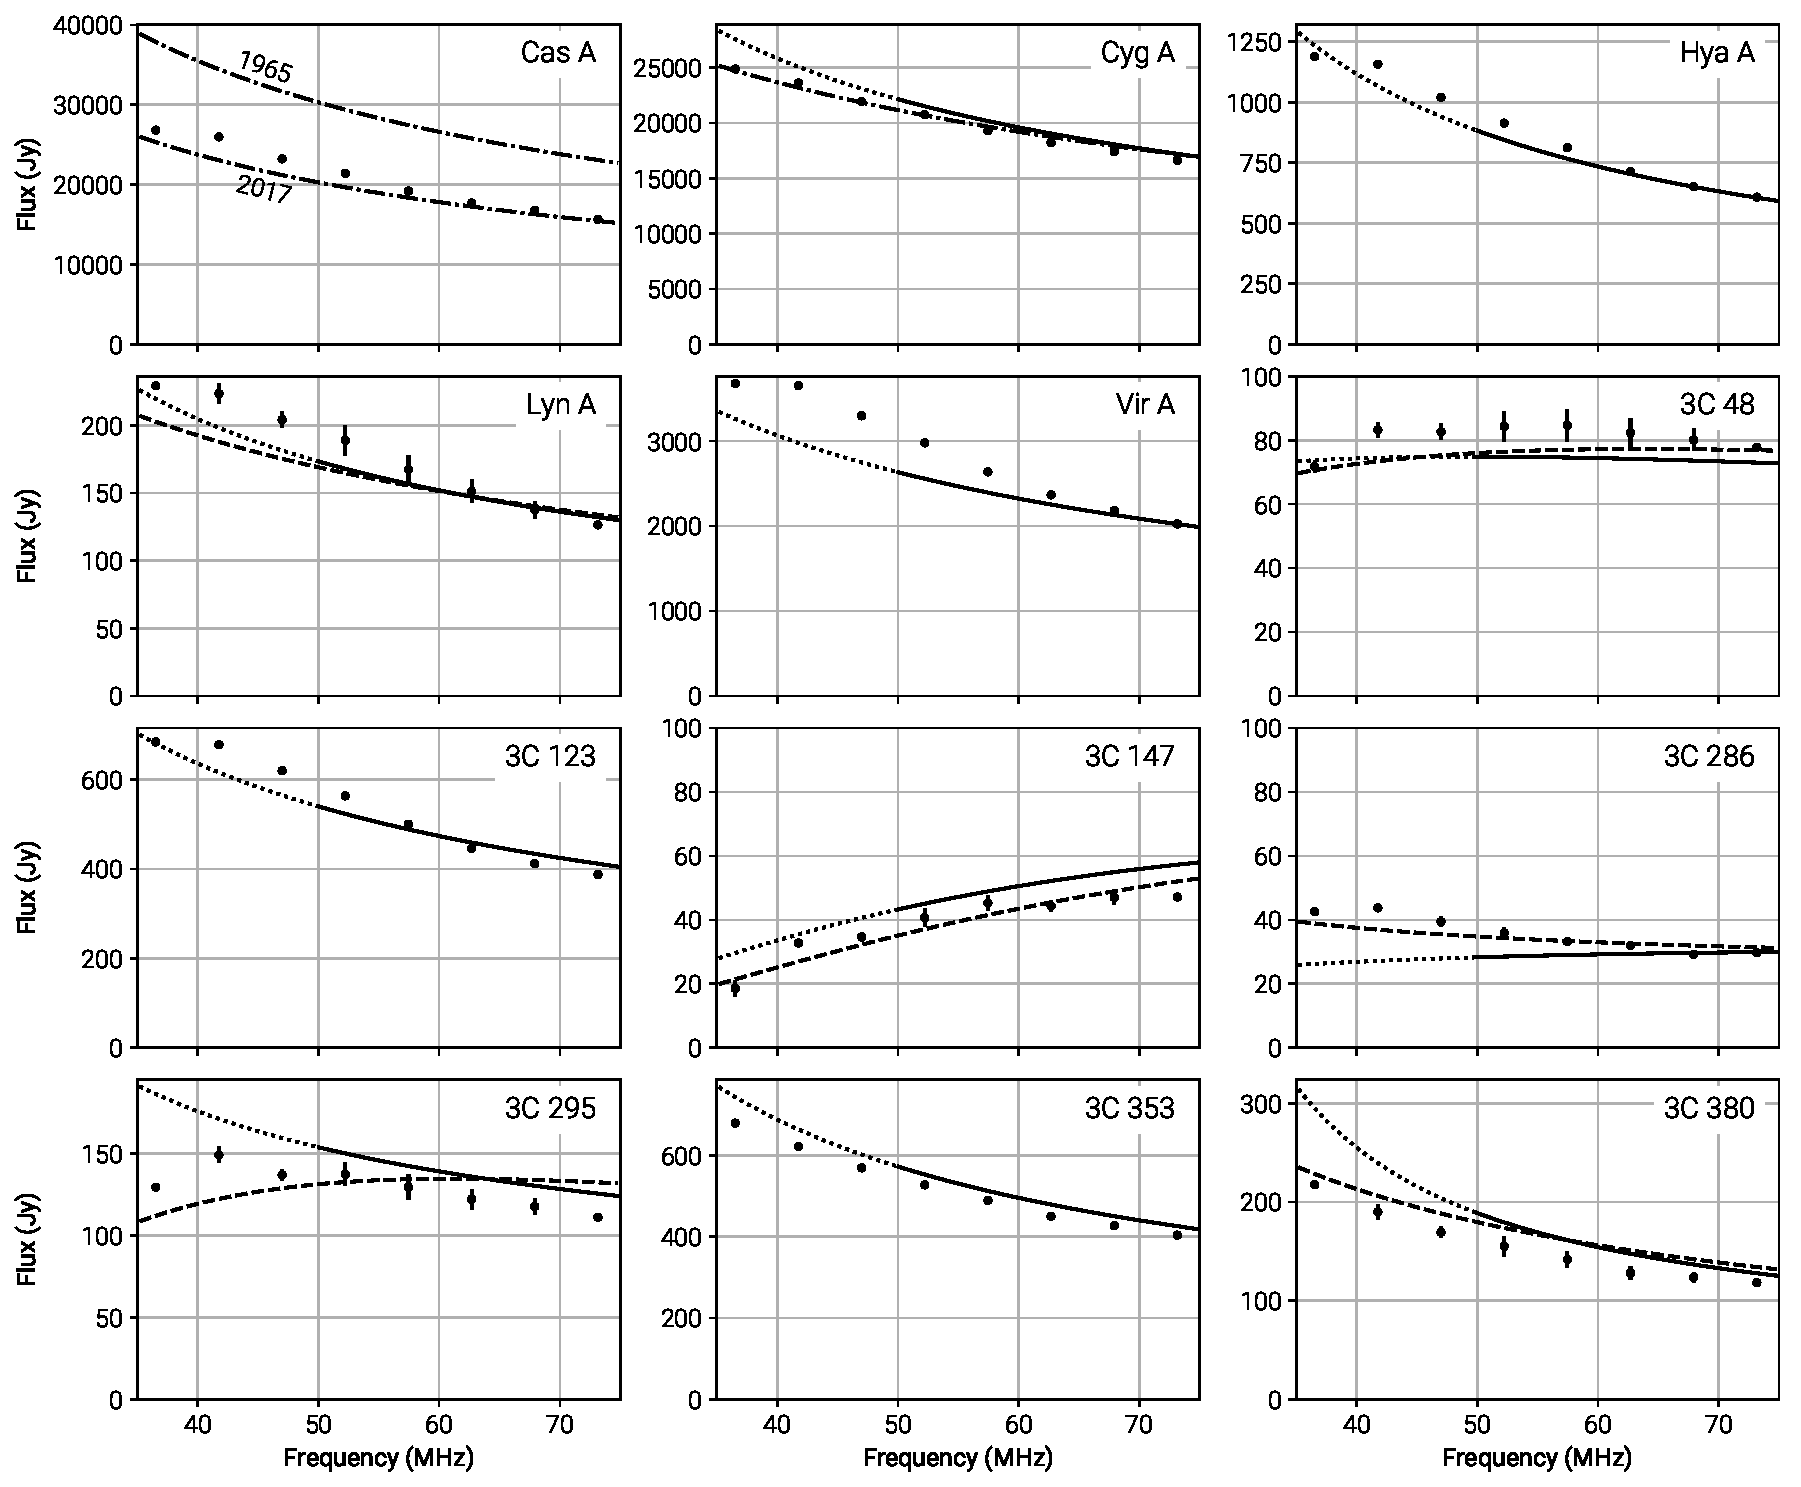
\includegraphics[width=\textwidth]{figures/chapter3/flux-scale}
    \caption{
        Measured fluxes (black points) of 11 sources plotted against the published spectra from
        \citet{2017ApJS..230....7P} (solid line above 50 MHz, dotted line below 50 MHz),
        \citet{2012MNRAS.423L..30S} (dashed line), and \citet{1977A&A....61...99B} (dot-dashed
        line).  Cas~A is compared against a spectrum assuming a secular decrease of 0.77\% per year
        \citep{2009AJ....138..838H}.
    }
    \label{fig:flux-scale}
\end{figure*}

The flux scale of the data was tied to the \citet{1977A&A....61...99B} spectrum of Cyg~A during gain
calibration. However, gain calibration is also a function of the beam model and the spectrum used
for Cas~A. Recent work by \citet{2012MNRAS.423L..30S} (hereafter SH12) using archival data from the
literature and \citet{2017ApJS..230....7P} (hereafter PB17) using the VLA has expanded the number of
low-frequency radio sources with calibrated flux measurements from one (Cyg~A) to 11 in total.
While the SH12 flux scale is valid between 30 and 300~MHz, the PB17 flux scale is somewhat more
limited because the lowest-frequency observations come from the VLA 4-band system. As a consequence,
the PB17 flux scale is not valid below 50 MHz.

Figure~\ref{fig:flux-scale} shows a comparison between flux measurements made using the all-sky maps
from this work and spectra from the aforementioned flux scales. Generally, the OVRO-LWA flux
measurements agree to between 5\% and 10\% of the SH12 spectra. Below 50 MHz, there can be substantial
departures with respect to the extrapolated PB17 spectra (e.g.,  3C 286, 3C 295, and 3C 380), but
it is usually the case that we have much better agreement with the SH12 spectra. This indicates that
the PB17 spectra cannot be extrapolated below 50 MHz.

%%%%%%%%%%%%%%%%%%%%%%%%%%%%%%%%%%%%%%%%%%%%%%%%%%%%%%%%%%%%%%%%%%%%%%%%%%%%%%%%%%%%%%%%%%%%%%%%%%%%
\section{Results}\label{sec:results}

\begin{figure*}[ht]
    \centering
    \begin{tabular}{c}
        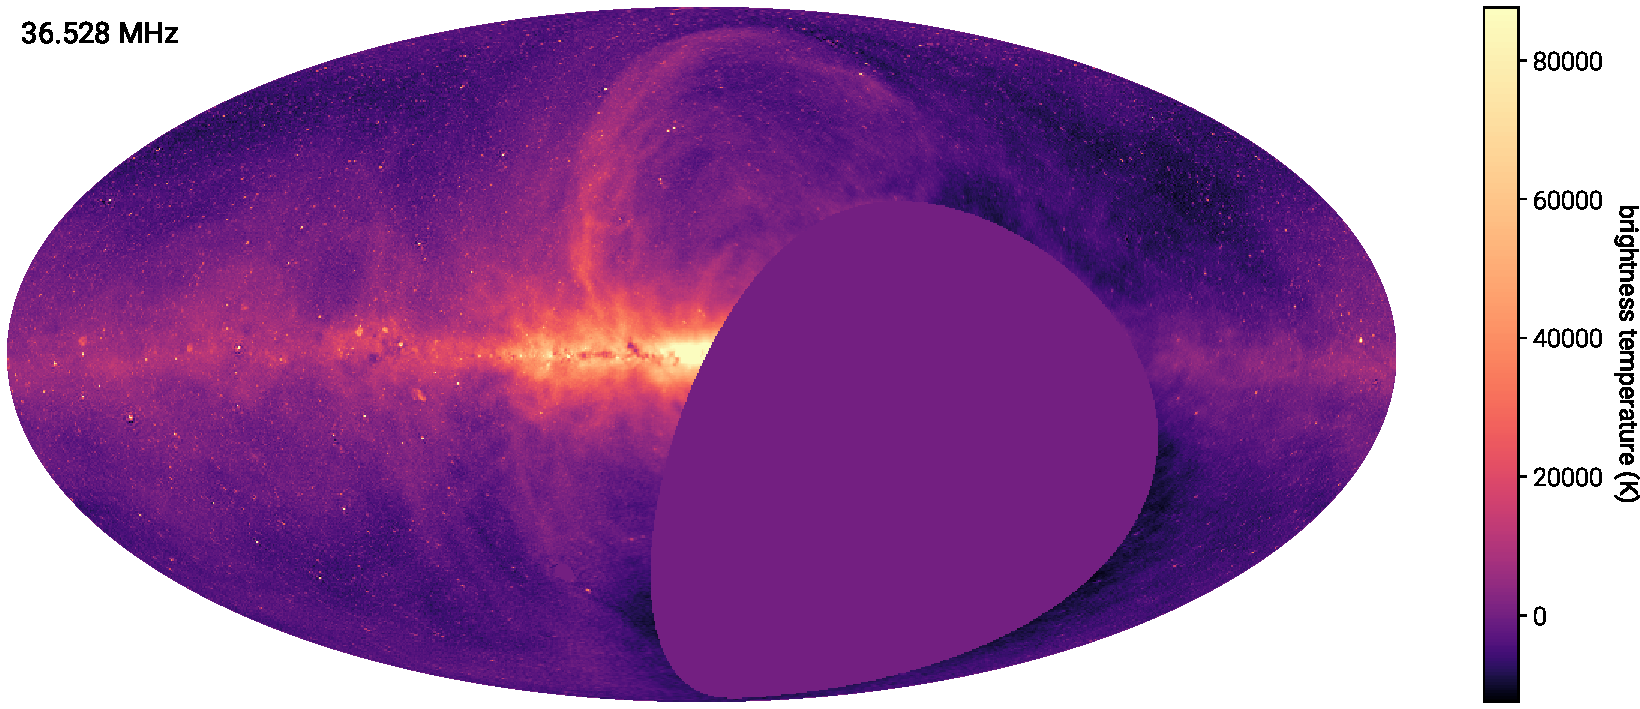
\includegraphics[height=0.32\textheight]{figures/chapter3/spw04} \\
        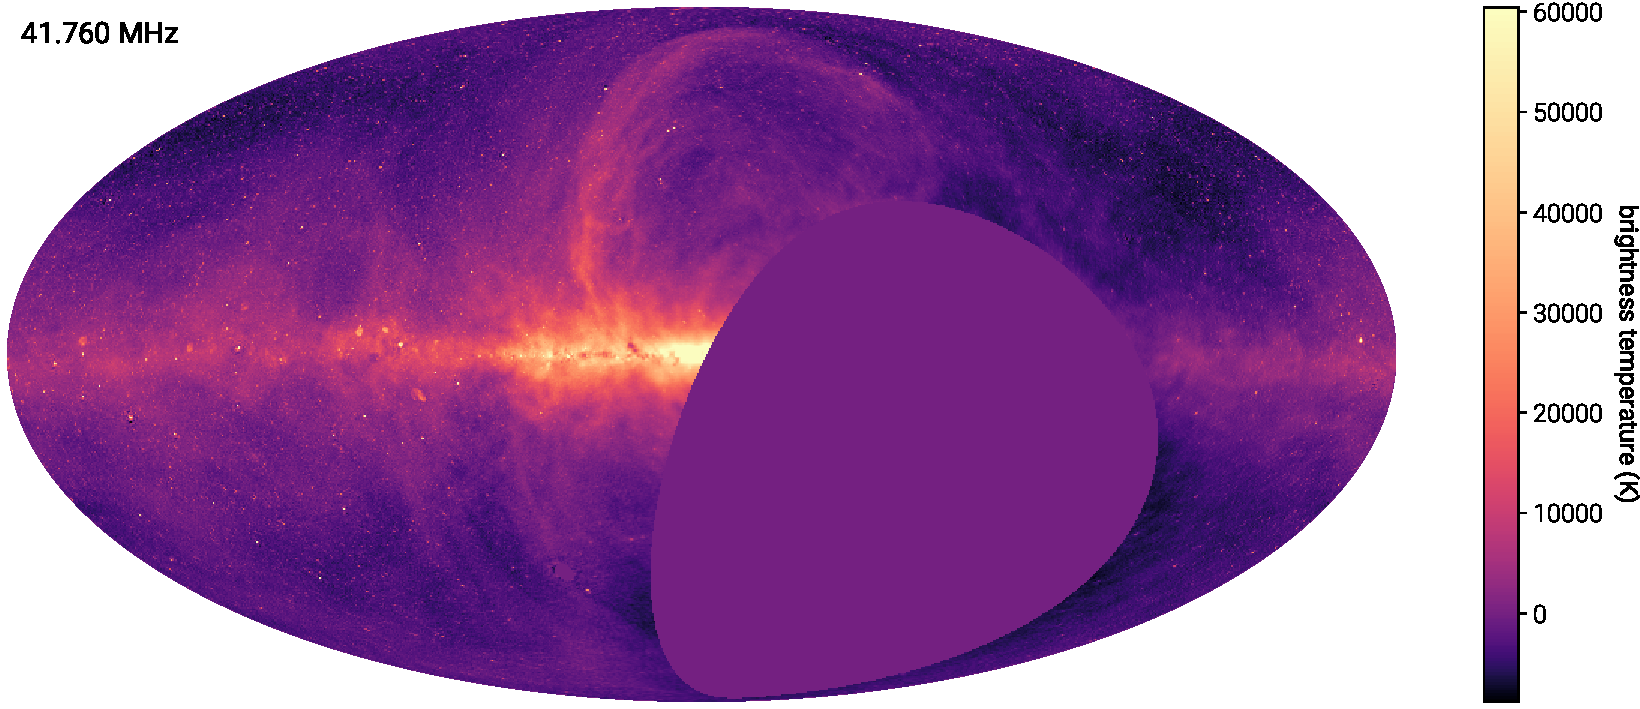
\includegraphics[height=0.32\textheight]{figures/chapter3/spw06} \\
    \end{tabular}
    \caption{
        These eight panels illustrate (with a Mollweide projection and logarithmic color scale) the
        eight full-sky maps generated with Tikhonov-regularized $m$-mode analysis imaging and the
        OVRO-LWA.  Each map covers the sky north of $\delta=-30^\circ$ with angular resolution of
        $\sim15\arcmin$. Eight bright sources have been removed from each map (Cyg~A, Cas~A, Vir~A,
        Tau~A, Her~A, Hya~A, 3C~123, and 3C~353). The small blank region near $l=+45.7^\circ$,
        $b=-47.9^\circ$ corresponds to the location of the Sun during the observation period.  A
        detailed summary of the properties of each map is given in Table~\ref{tab:summary}.
    }
    \label{fig:channel-maps}
\end{figure*}

\addtocounter{figure}{-1}
\begin{figure*}[p]
    \centering
    \begin{tabular}{c}
        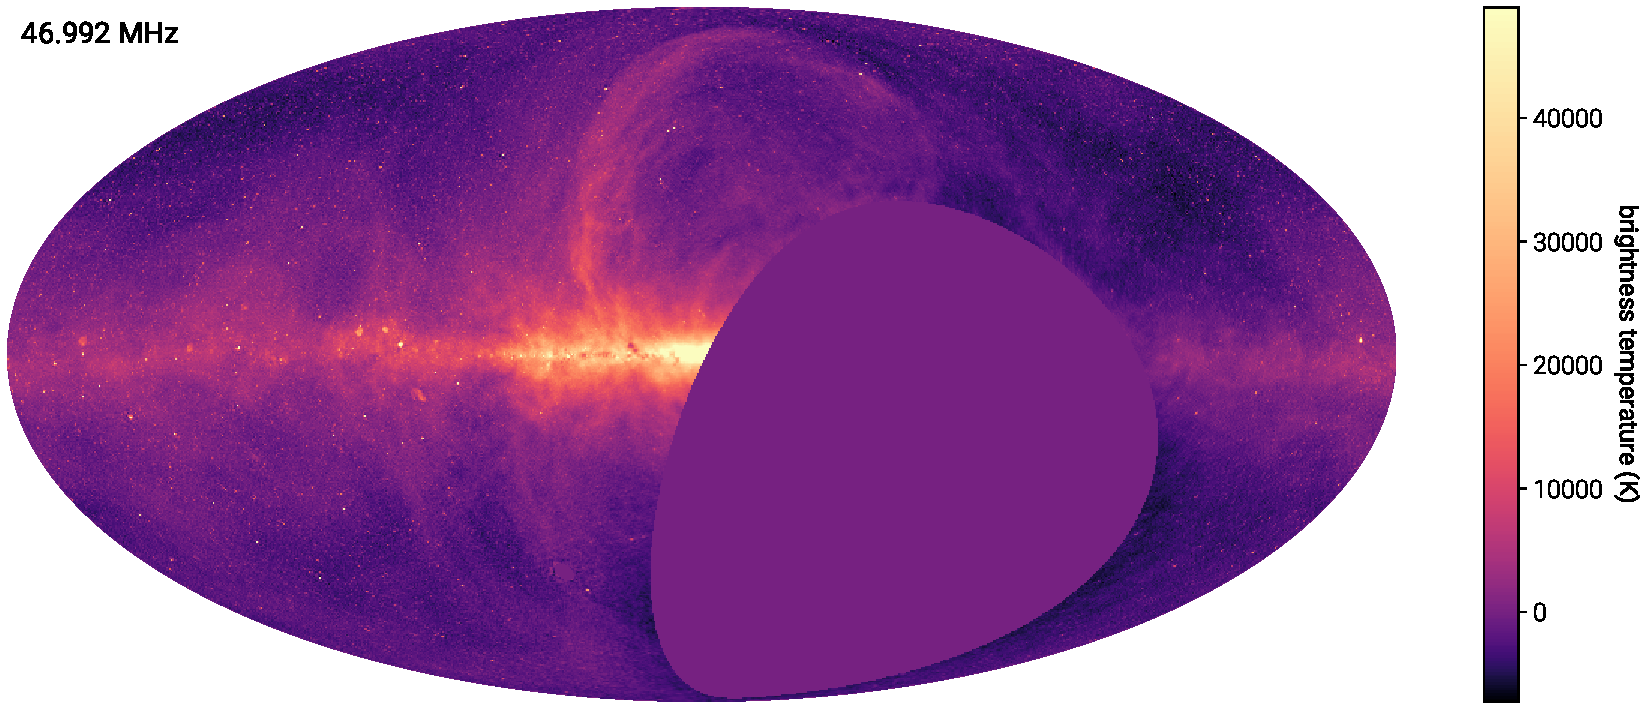
\includegraphics[height=0.32\textheight]{figures/chapter3/spw08} \\
        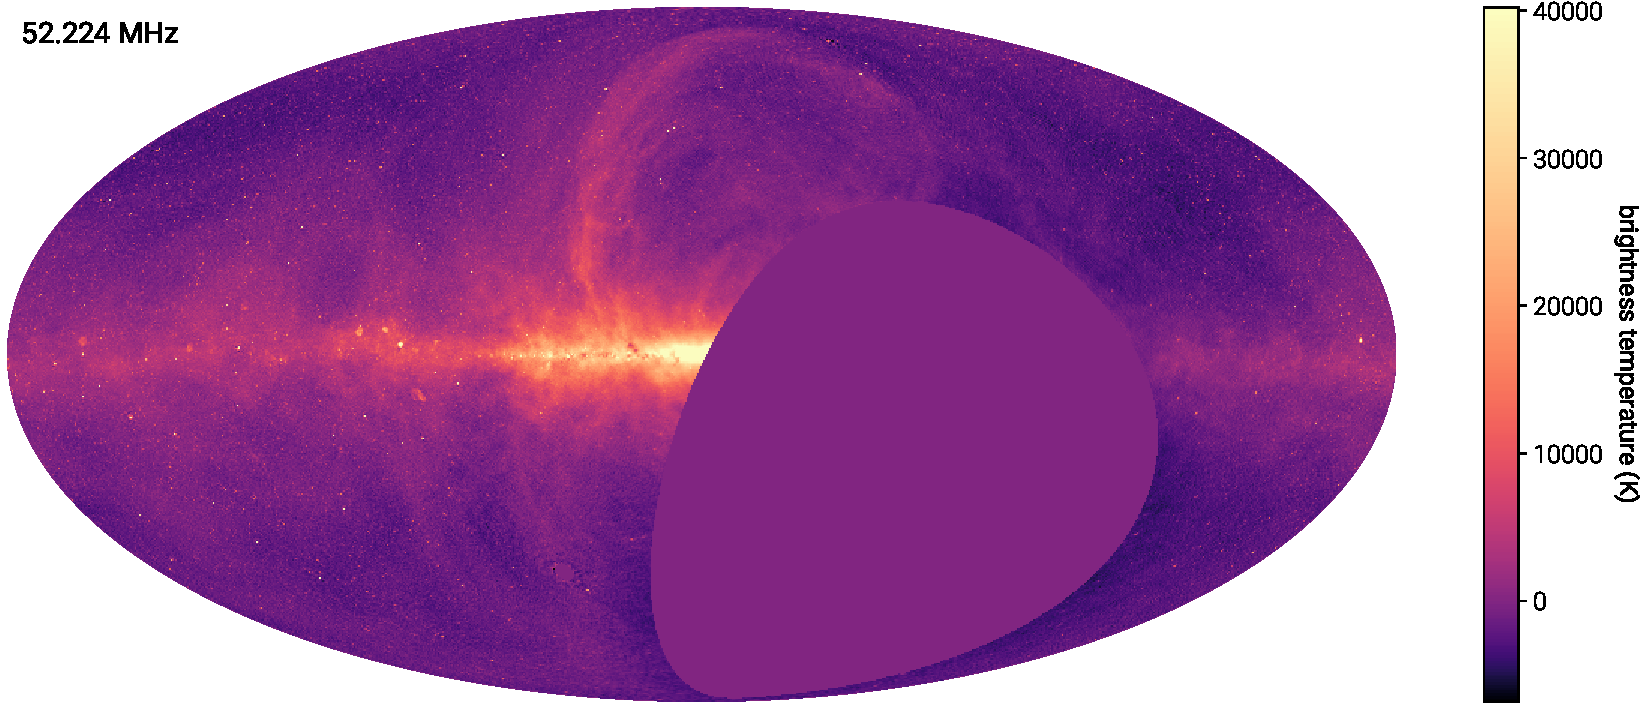
\includegraphics[height=0.32\textheight]{figures/chapter3/spw10} \\
        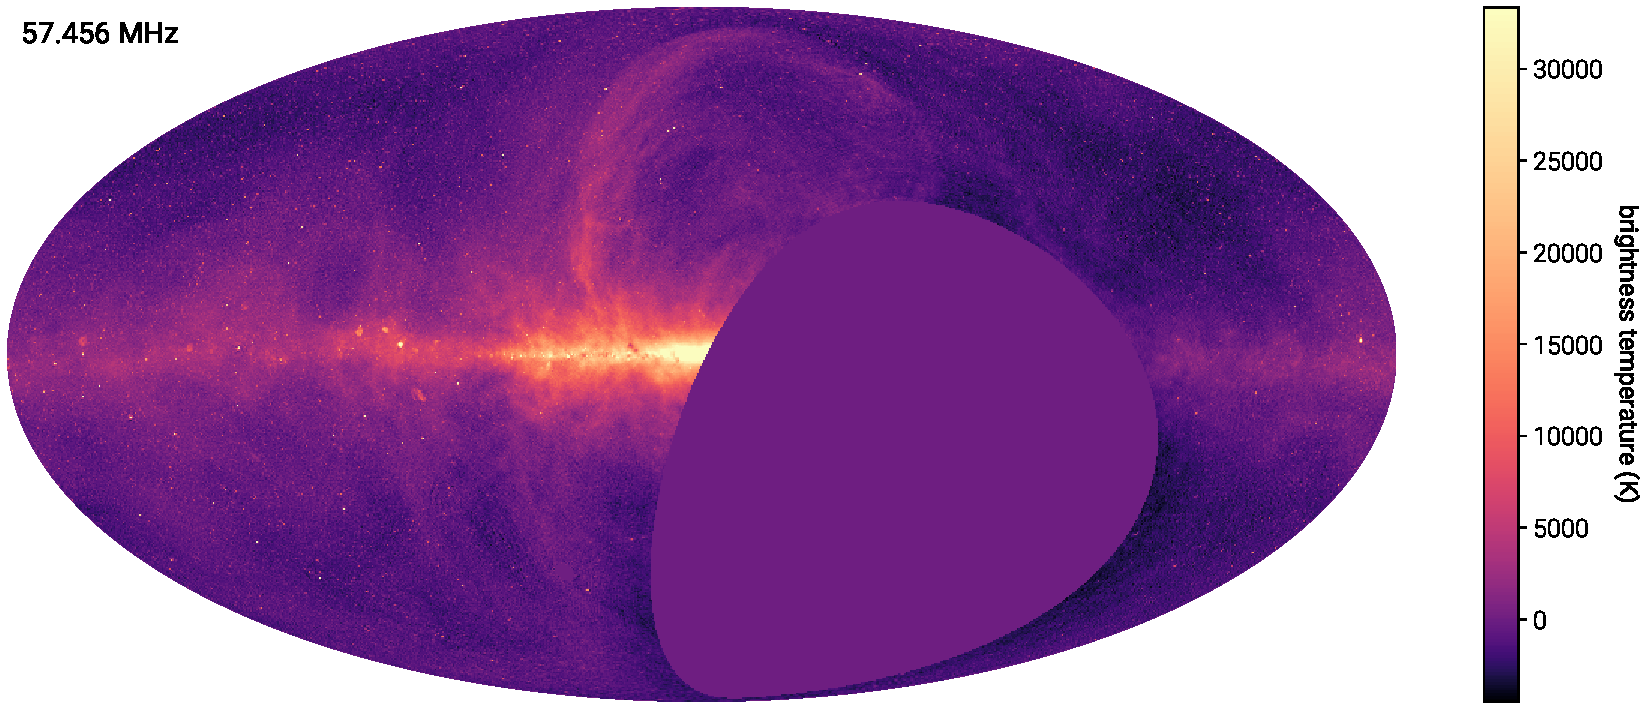
\includegraphics[height=0.32\textheight]{figures/chapter3/spw12} \\
    \end{tabular}
    \caption{
        continued
    }
\end{figure*}

\addtocounter{figure}{-1}
\begin{figure*}[p]
    \centering
    \begin{tabular}{c}
        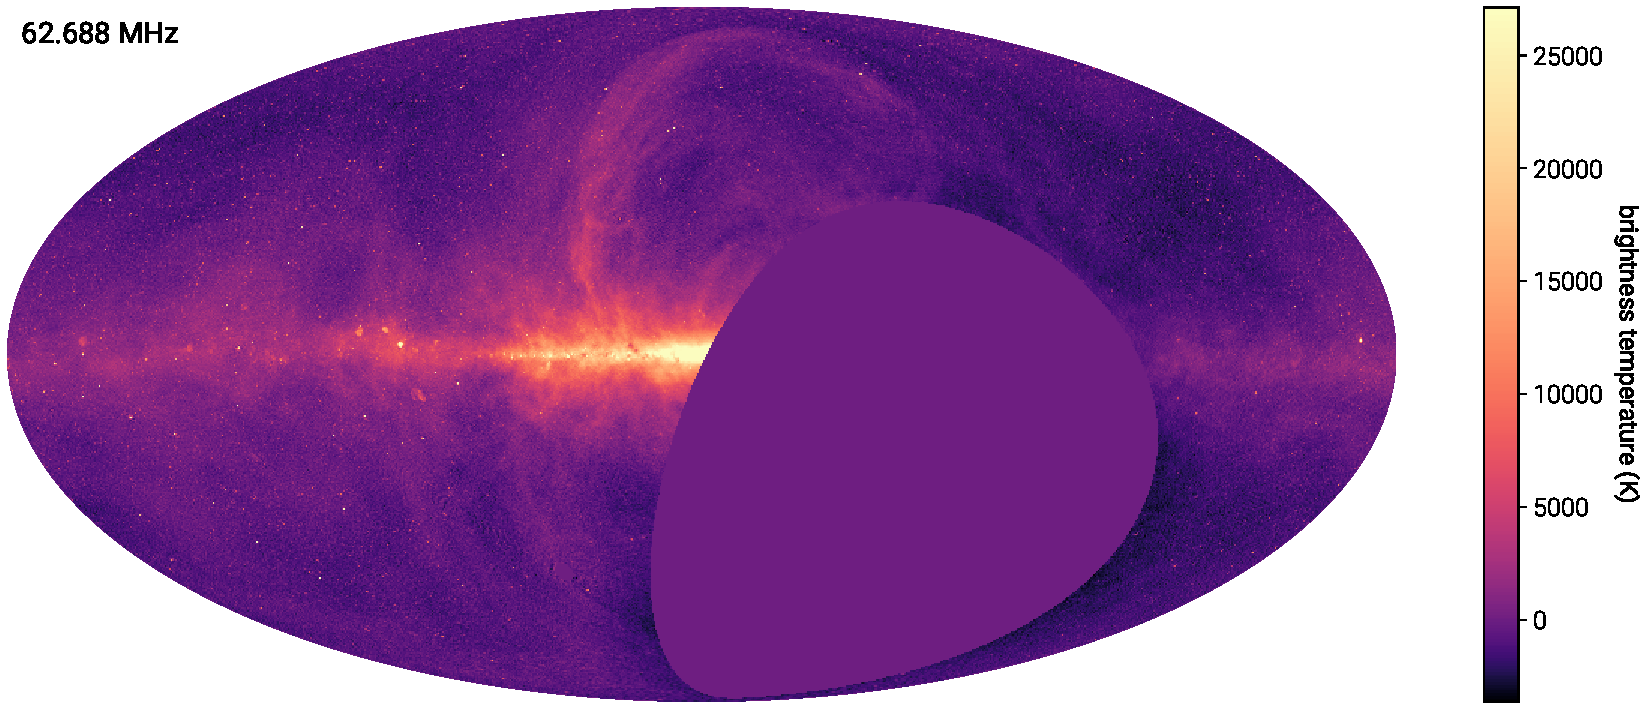
\includegraphics[height=0.32\textheight]{figures/chapter3/spw14} \\
        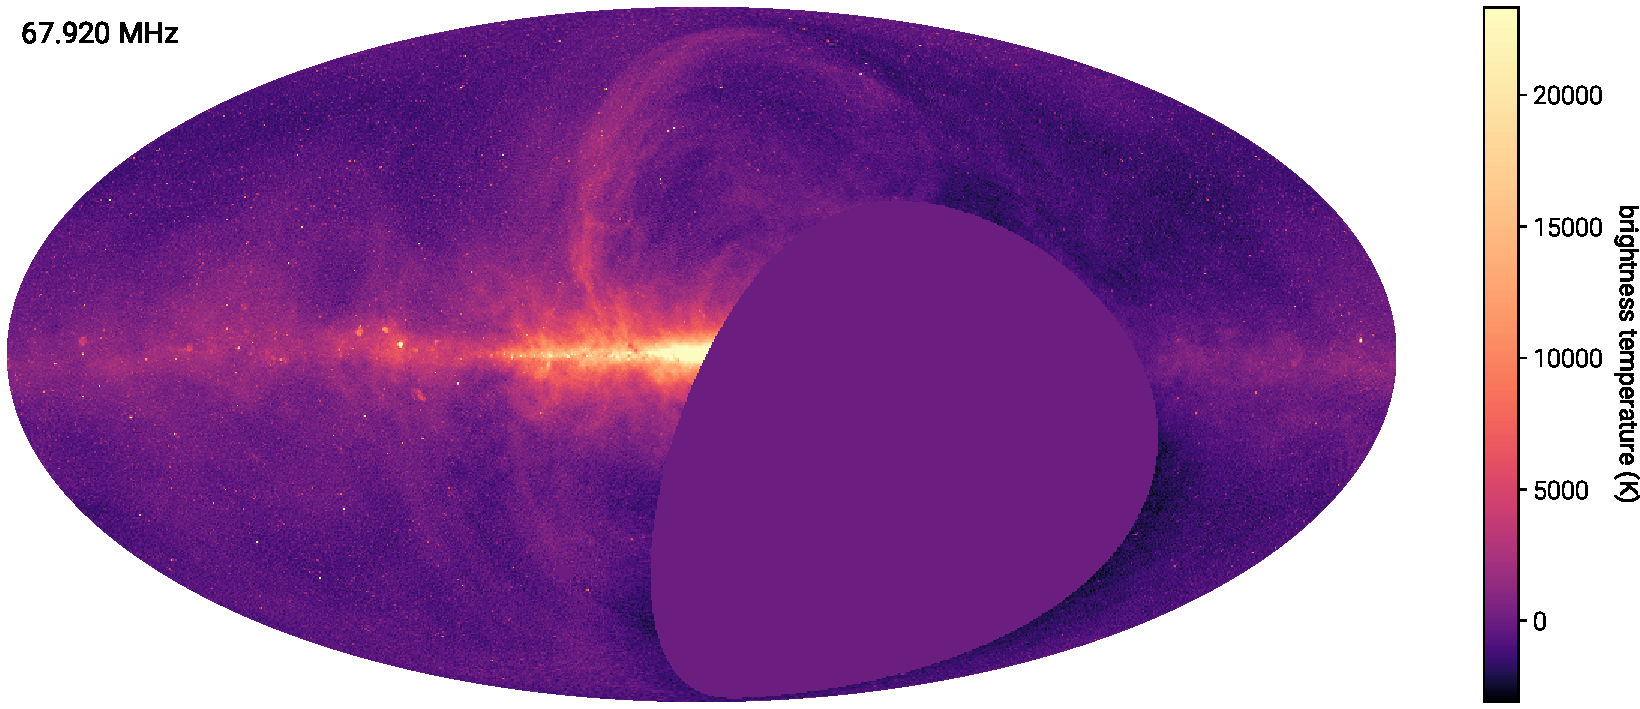
\includegraphics[height=0.32\textheight]{figures/chapter3/spw16} \\
        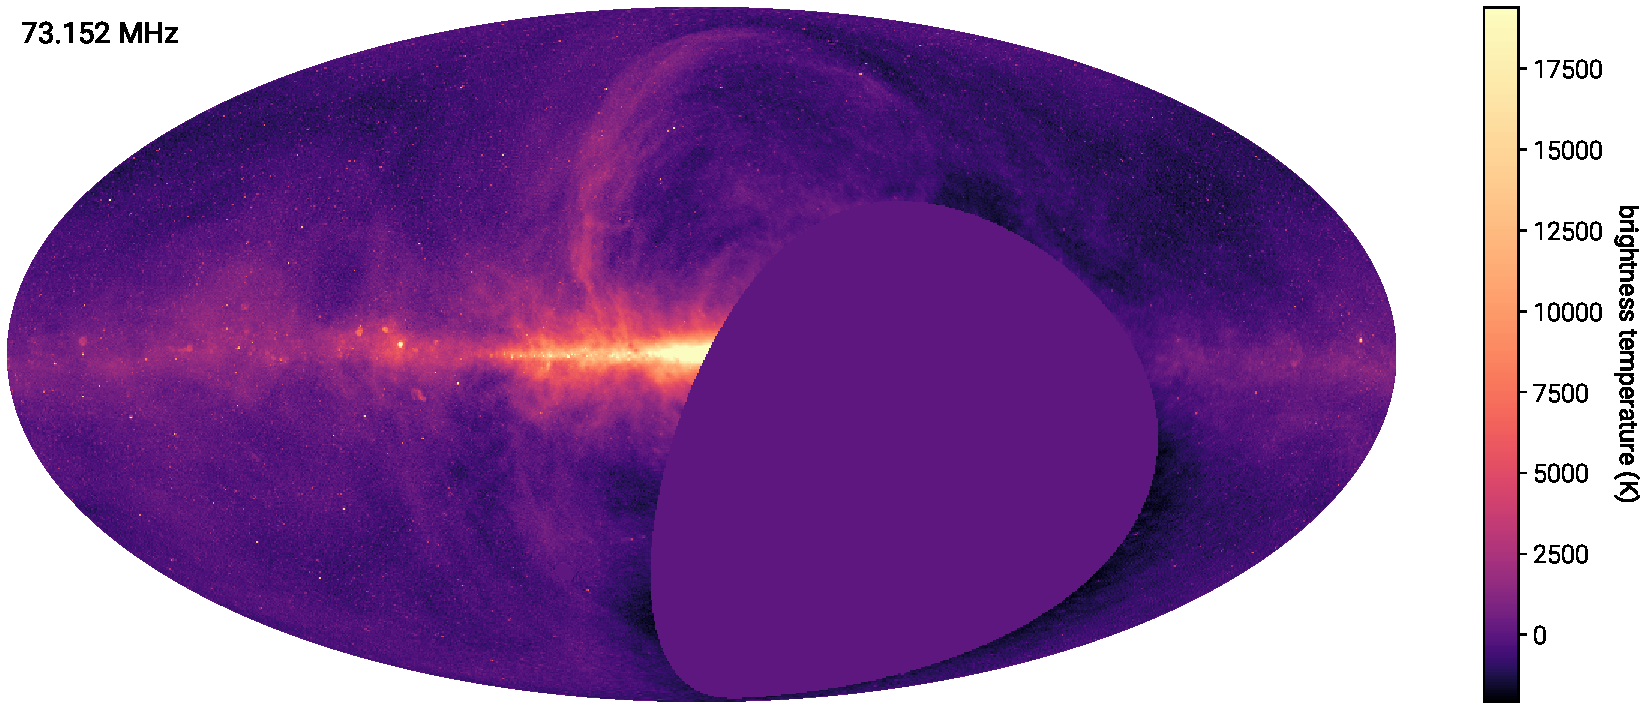
\includegraphics[height=0.32\textheight]{figures/chapter3/spw18} \\
    \end{tabular}
    \caption{
        continued
    }
\end{figure*}

\begin{figure*}[t]
    \centering
    \includegraphics[width=\textwidth]{figures/chapter3/ovro-lwa-sky-map.pdf}
    \caption{
        This Mollweide-projected map is constructed from three maps of the sky at 36.528~MHz (red),
        52.224~MHz (green), and 73.152~MHz (blue). The maps are scaled by $\nu^{2.5}$ before
        combining, and the color scale is logarithmic (as in Figure~\ref{fig:channel-maps}).
        Therefore, regions with a spectral index of $-2.5$ will tend to appear white, and regions
        with a flatter spectral index will tend to appear blue.
    }
    \label{fig:three-color}
\end{figure*}

\begin{figure*}[t]
    \centering
    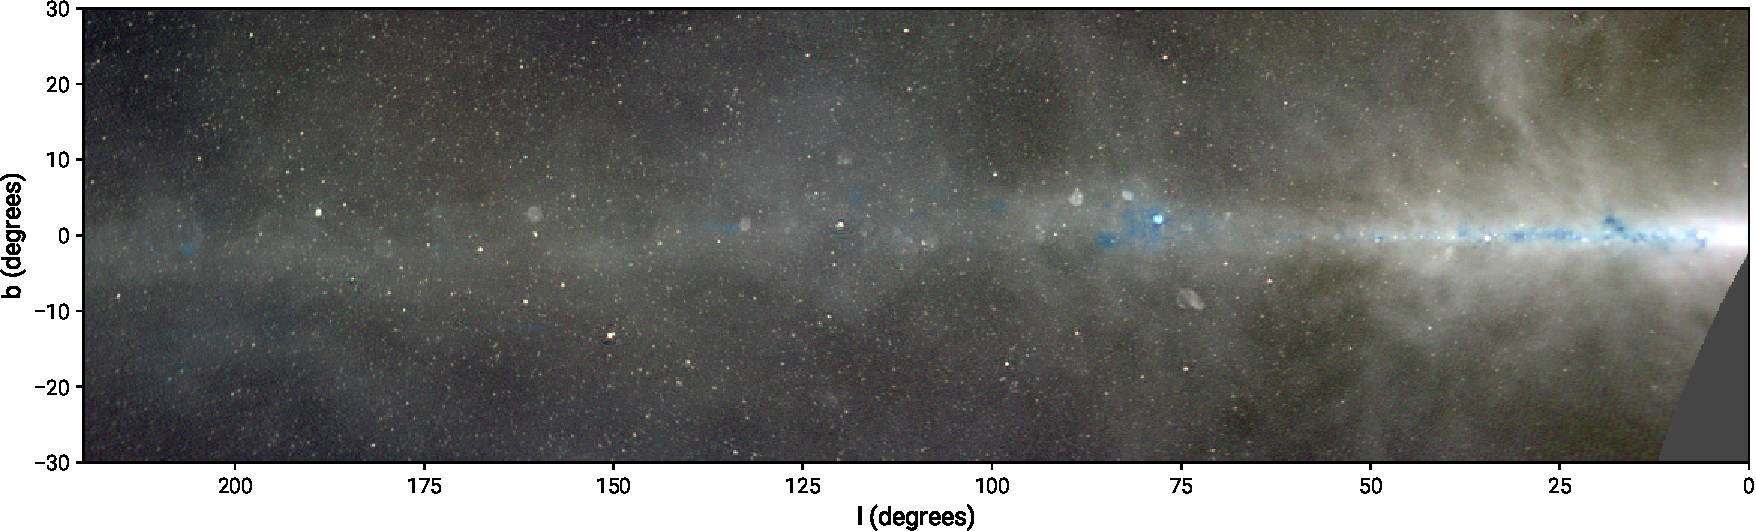
\includegraphics[width=\textwidth]{figures/chapter3/ovro-lwa-galactic-plane.pdf}
    \caption{
        Cutout of the galactic plane from Figure~\ref{fig:three-color}.
    }
    \label{fig:galactic-plane-cutout}
\end{figure*}

\begin{figure*}[t]
    \centering
    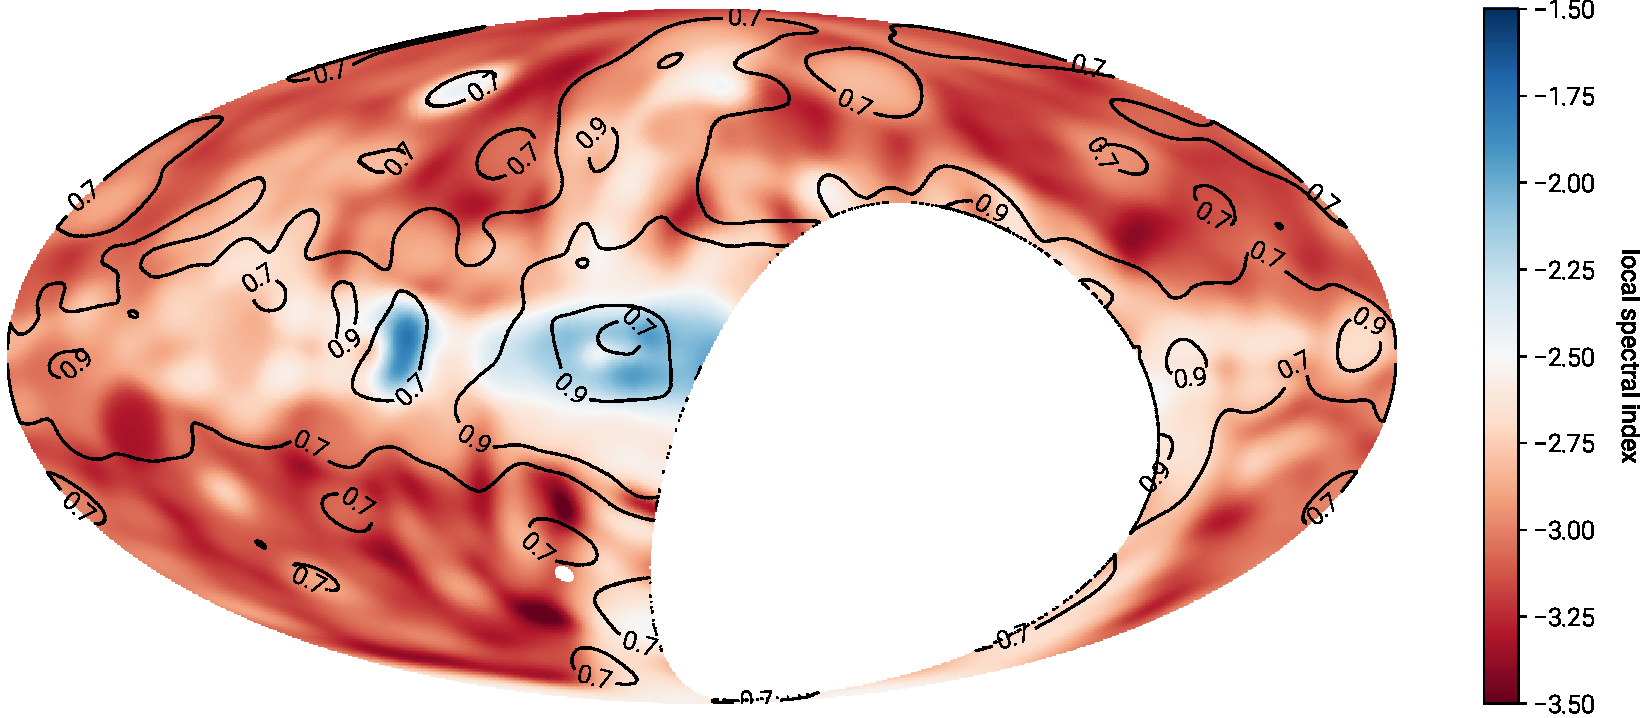
\includegraphics[width=\textwidth]{figures/chapter3/better-internal-spectral-index}
    \caption{
        Local spectral index measured between the 36.528~MHz map and the 73.152~MHz map estimated by
        means of a local T--T plot. The color scale gives the spectral index, where blue is flat
        spectrum and red is steep spectrum. The contours give the coefficient of determination
        ($R^2$) for the linear fit to the local T--T plot. If $R^2$ is low, the quality of the fit
        is low, and the estimated spectral index is unreliable. This can be due to either
        insufficient dynamic range in the local T--T plot or multiple emission mechanisms operating
        in close proximity. Consequently, $R^2$ tends to drop at higher galactic latitudes (due to
        dynamic range) and near \ion{H}{2} regions in the galactic plane (due to multiple emission
        mechanisms).
    }
    \label{fig:internal-spectral-index}
\end{figure*}

\begin{figure*}[t]
    \centering
    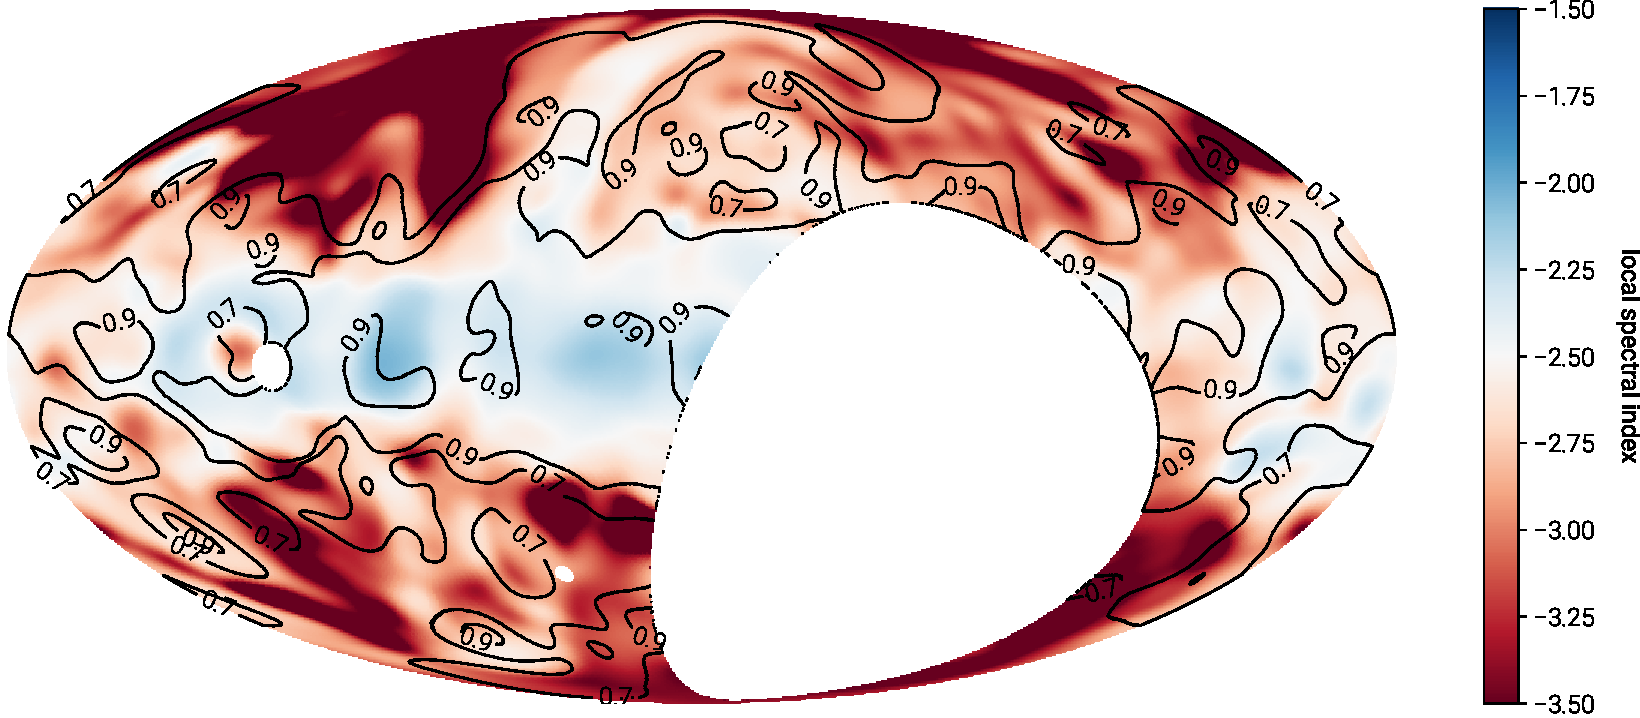
\includegraphics[height=0.32\textheight]{figures/chapter3/better-haslam-spectral-index}
    \caption{
        Local spectral index measured between the 73.152~MHz OVRO-LWA map and the reprocessed
        408~MHz Haslam map \citep{2015MNRAS.451.4311R}.  The color scale gives the spectral index,
        where blue is flat spectrum and red is steep spectrum. The contours give the coefficient of
        determination ($R^2$) for the linear fit to the local T--T plot. See the caption of
        Figure~\ref{fig:internal-spectral-index} for more details about the coefficient of
        determination.
    }
    \label{fig:haslam-spectral-index}
\end{figure*}

\begin{table*}[t]
    \centering
    \begin{tabular}{cccccccccc}
        \hline
        \hline
        & \tbf{$\b\nu$}
        & \tbf{$\b\Delta\b\nu$}\footnote{
            Bandwidth used to construct the map. As described in the text, each map is constructed
            from a single frequency channel (24~kHz).
        }
        & \multicolumn3c{\tbf{FWHM}\footnote{
            The full width at half maximum (FWHM) of the synthesized beam at the specified declination
            (major axis $\times$ minor axis).
        }}
        && \multicolumn2c{\tbf{Noise}\footnote{
            Measured with a jackknife and splitting the data set into even- and odd-numbered
            integrations. This estimate therefore includes all noise sources that act on the
            timescale of a single 13~s integration (e.g., thermal, ionospheric, etc.).
        }}
        & \tbf{Fraction of Modes}\footnote{
            Singular values of the transfer matrix compared with the value of the regularization
            parameter $\varepsilon$ used while solving Equation~\ref{eq:tikhonov-solution}. As
            discussed in the text, singular vectors with corresponding singular values $\sigma \ll
            \sqrt{\varepsilon}$ are set to zero by the Tikhonov regularization procedure.
        } \\
        \cline{4-6}
        \cline{8-9}
        \tbf{\#}
            & MHz & MHz
            & $\delta=0^\circ$ & $\delta=+45^\circ$ & $\delta=+75^\circ$
            && K & mJy/beam
            & with $\sigma>\sqrt{\varepsilon}$ \\
        \hline
        1 & 36.528 & 0.024 & $26.0'\times19.1'$ & $20.2'\times16.9'$ & $19.8'\times18.7'$ && 595. & 799. & 0.391 \\
        2 & 41.760 & 0.024 & $23.3'\times17.5'$ & $18.5'\times16.0'$ & $18.3'\times17.4'$ && 541. & 824. & 0.480 \\
        3 & 46.992 & 0.024 & $20.9'\times16.3'$ & $17.4'\times15.2'$ & $17.6'\times16.9'$ && 417. & 717. & 0.504 \\
        4 & 52.224 & 0.024 & $18.7'\times15.2'$ & $16.2'\times15.0'$ & $16.0'\times15.8'$ && 418. & 814. & 0.535 \\
        5 & 57.456 & 0.024 & $18.0'\times14.9'$ & $15.9'\times15.0'$ & $15.7'\times15.4'$ && 354. & 819. & 0.542 \\
        6 & 62.688 & 0.024 & $17.8'\times15.0'$ & $15.8'\times14.9'$ & $15.7'\times15.4'$ && 309. & 843. & 0.540 \\
        7 & 67.920 & 0.024 & $17.6'\times15.0'$ & $15.9'\times14.7'$ & $15.8'\times15.6'$ && 281. & 894. & 0.529 \\
        8 & 73.152 & 0.024 & $18.6'\times15.1'$ & $16.8'\times14.6'$ & $16.6'\times16.1'$ && 154. & 598. & 0.512 \\
        \hline \hline
    \end{tabular}
    \caption{A summary of the generated all-sky maps.}
    \label{tab:summary}
\end{table*}

We constructed eight sky maps using Tikhonov-regularized $m$-mode analysis imaging and CLEANing with
observations from the OVRO-LWA. Each map is individually shown in Figure~\ref{fig:channel-maps},
Figure~\ref{fig:three-color} is a three-color image constructed from the maps at 36.528,
52.224, and 73.152~MHz, and Figure~\ref{fig:galactic-plane-cutout} is a cutout of the galactic
plane. The maps cover the sky north of $\delta=-30^\circ$ with $\sim 15\arcmin$ angular resolution.
The eight brightest northern hemisphere point sources are removed from each map (Cyg~A, Cas~A,
Vir~A, Tau~A, Her~A, Hya~A, 3C~123, and 3C~353), as described in \S\ref{sec:source-removal}, and
there is a small blank region near $l=+45.7^\circ$, $b=-47.9^\circ$ corresponding to the position of
the Sun during the observing window. The properties of each map -- including frequency, bandwidth,
angular resolution, and thermal noise -- are presented in Table~\ref{tab:summary}.

Each map from Figure~\ref{fig:channel-maps} will be made freely available online in Healpix format
\citep{2005ApJ...622..759G} on LAMBDA.

Due to the considerations presented by \citet{2016ApJ...826..116V} and discussed in
\S\ref{sec:mmode-analysis}, each of these maps is monopole-subtracted ($a_{00}=0$).  Furthermore, in
order to suppress sources of terrestrial interference, all spherical harmonics with $m=0$, or $m=1$
and $l>100$ are filtered from the map (where the spherical harmonics are defined in the J2017
coordinate system). As will be discussed in \S\ref{sec:rfi}, these spherical harmonics are
particularly susceptible to contamination by radio-frequency interference (RFI) and common-mode
pickup. As a consequence, astronomical emission that circles the J2017 north celestial pole (NCP) is
filtered from the maps.  This filtering creates negative rings around the NCP at the declination of
bright point sources.  These rings are naturally removed from the map during CLEANing as long as
this filtering step is included in the PSF calculation.

The noise in each map is empirically measured using jackknife resampling. The data set is first split
into even- and odd-numbered integrations. These two groups are then imaged and CLEANed
independently before being compared against the maps constructed from all of the available data
using the jackknife standard error estimator. This estimate of the standard error includes all
sources of error that operate on $\sim13$~s timescales (the integration time), such as thermal
noise and rapid ionospheric fluctuations, but does not account for more slowly varying effects (for
example, sidereal variation in the system temperature or day--night fluctuations in the ionosphere).
These noise calculations are summarized in Table~\ref{tab:summary}.  VLSSr source counts
\citep{2014MNRAS.440..327L} suggest that the confusion limit at 74 MHz and 15\arcmin angular
resolution is $\sim 1000\times(\nu/74\,{\rm MHz})^{-0.7}$ mJy.  Each channel map achieves thermal
noise $<900$~mJy; therefore, each map is likely at or near the confusion limit.

In the absence of a zero-level correction, a pixel-by-pixel power-law fit to the new maps is
impossible. In general, this zero-level correction requires calibrated total power measurements that
will be included in future work.  Instead, temperature--temperature plots (T--T plots) can be used
to measure the spectral index independently of any zero-level corrections
\citep{1962MNRAS.124..297T}.  This method relies on the assumption that all pixels in a given region
are described by the same power law. In that case, there exists a linear relationship between the
brightness temperature at frequency $\nu_1$ and frequency $\nu_2$. The slope of this best-fit line
is a measure of the spectral index between the two frequencies. The T--T plot can fail to obtain a
reliable measure of the spectral index in two ways.  First, if there is not enough dynamic range in
the emission region, there may be only a weak correlation between the brightness temperature at
$\nu_1$ and $\nu_2$.  Second, if two emission mechanisms operate in close proximity (i.e.,
synchrotron and free-free), then a single power-law interpretation of the emission in that region
will be poor. Consequently, spectral indices estimated from T--T plots can require careful
interpretation.

In Figure~\ref{fig:internal-spectral-index}, the spectral index is locally estimated in each part of
the sky within a region $\sim10^\circ$ across by constructing local T--T plots between 36.528 and
73.152~MHz. Contours of constant $R^2$ (the coefficient of determination) are overlaid. If $R^2\sim
1$, the spectral index is reliable because there is locally a strong linear correlation between
36.528 and 73.152~MHz. However, if $R^2\ll 1$, the spectral index calculation is unreliable.  $R^2$
tends to drop in cold patches of the sky where there is not enough dynamic range to find a strong
correlation between the two frequencies. It also  ends to drop in the vicinity of \ion{H}{2} regions
in the galactic plane due to multiple emission mechanisms violating the assumption of a single
spectral index. Therefore, we should restrict our interpretation of
Figure~\ref{fig:internal-spectral-index} to the galactic plane and north galactic spur. In the
galactic plane, the synchrotron spectral index varies between $\sim-2.5$ and $-2.75$. In the
vicinity of \ion{H}{2} regions, the spectral index flattens significantly.  These \ion{H}{2} regions
can be seen with higher resolution in Figure~\ref{fig:galactic-plane-cutout}. In
Figure~\ref{fig:galactic-plane-cutout}, \ion{H}{2} regions appear as blue shadows along the galactic
plane due to the increasing impact of free-free absorption at lower frequencies.

In the literature, the spectral index at low frequencies is commonly computed with respect to the
Haslam 408~MHz map \citep{1981A&A...100..209H, 1982A&AS...47....1H}, which was reprocessed by
\citet{2015MNRAS.451.4311R} to remove artifacts associated with $1/f$ noise and bright sources.
Figure~\ref{fig:haslam-spectral-index} displays the spectral index computed between the 73.152~MHz
map and the reprocessed Haslam map. The spectral index was estimated by degrading the 73.152~MHz map
to the resolution of the Haslam map and constructing local T--T plots in every direction. The
coefficient of determination is overlaid as a contour plot; however, because
$\log(408\,\text{MHz}/73.152\,\text{MHz}) > \log(73.152\,\text{MHz}/36.528\,\text{MHz})$, the
spectral indices presented in Figure~\ref{fig:haslam-spectral-index} tend to be more robust than
those presented in Figure~\ref{fig:internal-spectral-index}. This is reflected by the fact that
$R^2$ is larger, but the interpretation must still generally be restricted to the galactic plane.

\subsection{Comparisons with Other Sky Maps}\label{sec:compare}

\subsubsection{LWA1 Low Frequency Sky Survey}

\begin{figure*}[t]
    \centering
    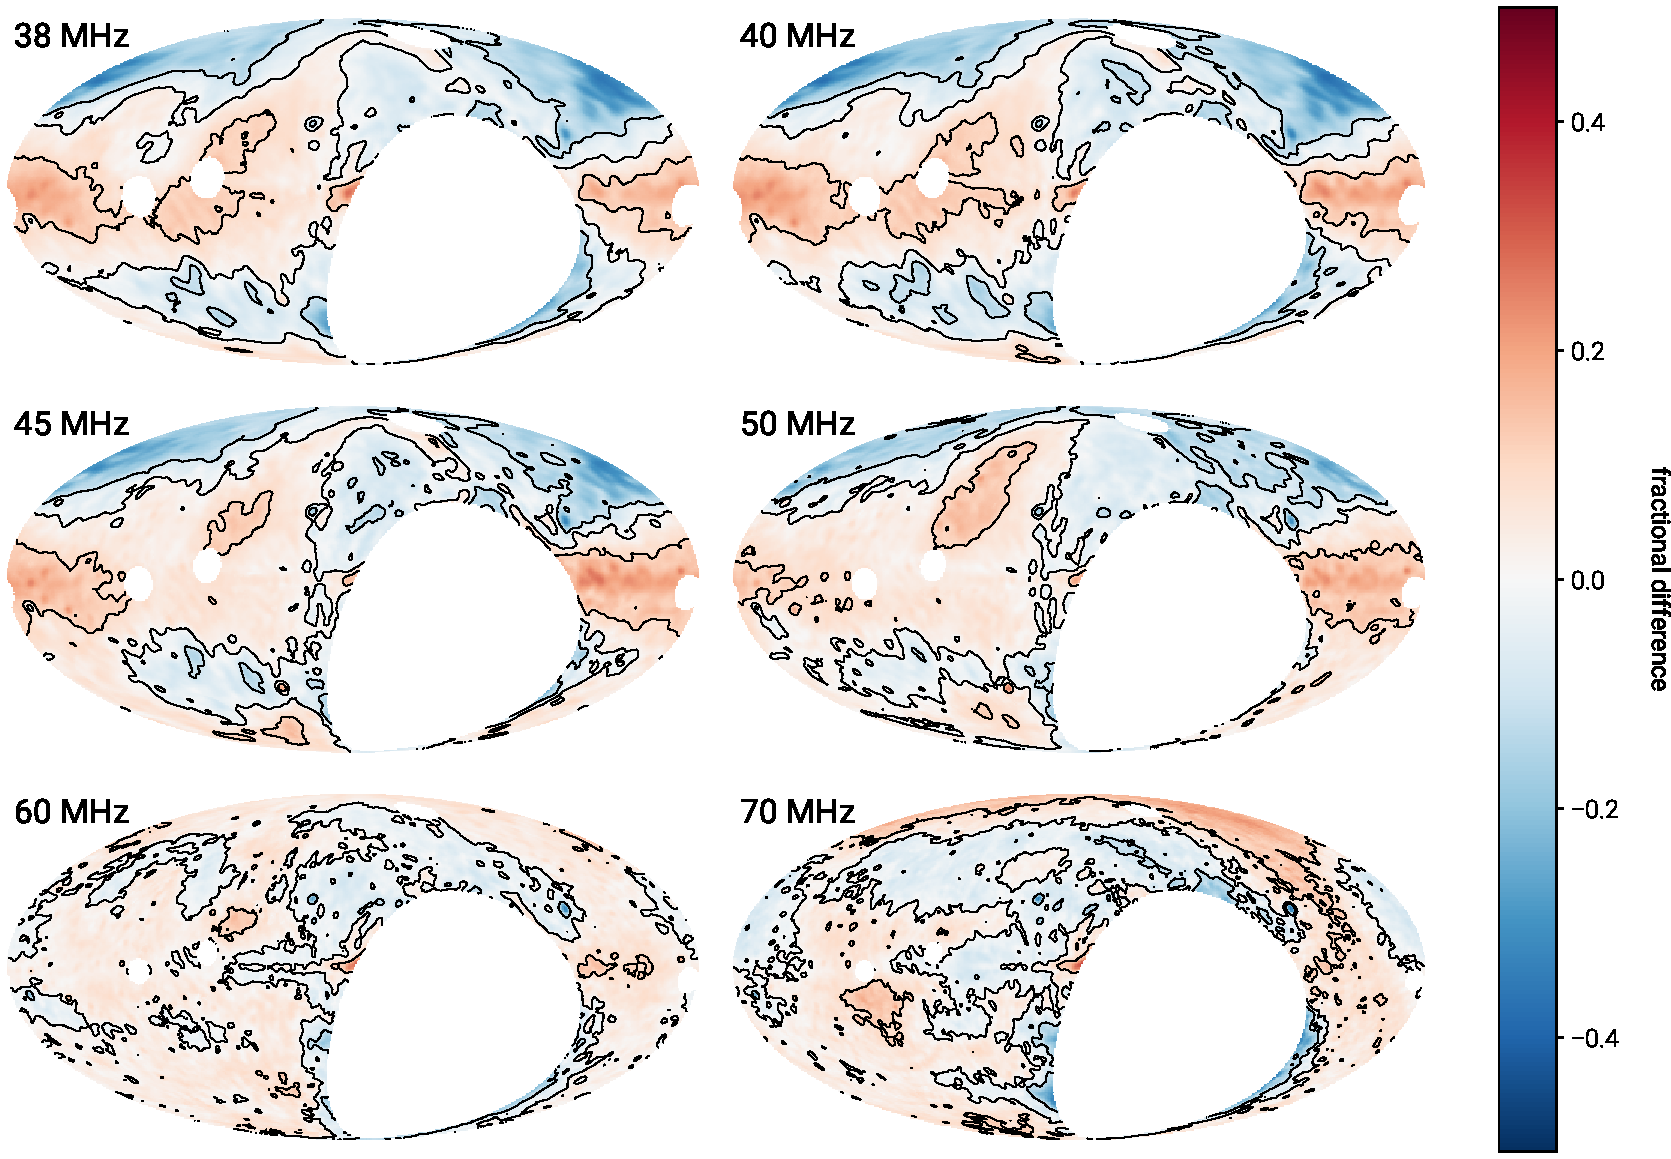
\includegraphics[width=\textwidth]{figures/chapter3/lwa1}
    \caption{
        Fractional difference between maps from the LLFSS and the OVRO-LWA maps
        (Figure~\ref{fig:channel-maps}) after interpolating to the corresponding frequency and
        smoothing to the corresponding resolution. A positive value indicates regions where the
        OVRO-LWA map has more emission that the corresponding LLFSS map. Cas A, Cyg A, Vir A, and
        Tau A are masked due to the fact that they are subtracted from the OVRO-LWA maps.
    }
    \label{fig:lwa1-comparison}
\end{figure*}

The LWA1 Low Frequency Sky Survey \citep[LLFSS;][]{2017MNRAS.469.4537D} produced nine maps of the
sky between 35 and 80~MHz. Six of these maps are interior to the frequency range spanned by this
work. Initial comparisons with the LLFSS helped characterize a systematic rotation in the LWA1's
antenna positions. After phase calibration, this manifested itself as a systematic rotation and
translation in the snapshot images that were mosaicked to form the final sky map. This systematic
error has been corrected in the comparisons presented here and in the latest version of the
LLFSS.\footnote{
    Available for download at \url{http://lda10g.alliance.unm.edu/LWA1LowFrequencySkySurvey/}
}

A direct comparison with these updated LLFSS maps can be seen in Figure~\ref{fig:lwa1-comparison}.
In this figure, the LLFSS maps are filtered to remove the monopole and all modes with $m=0$. The
OVRO-LWA maps are interpolated in frequency and blurred to match the angular resolution of the
corresponding LLFSS map.  At 60~MHz, the agreement is generally better than 10\%. However, at lower
frequencies the agreement deteriorates to about 20\%.  Typically, the OVRO-LWA maps have excess
emission in the galactic plane and a deficit of emission off the galactic plane relative to the
LLFSS.

The LLFSS incorporates calibrated total power radiometry to estimate the missing flux from short
spacings. As a result, \citet{2017MNRAS.469.4537D} reported per-pixel spectral indices from combining
all nine sky maps. Care must be taken in comparing these spectral indices with
Figure~\ref{fig:internal-spectral-index} because they are susceptible to different systematic
errors. Both calculations are sensitive to mistakes in the antenna primary beam, but the LLFSS
spectral indices are additionally sensitive to errors in the zero level. We will restrict the
comparison to the galactic plane where the spectral indices are likely to be the most reliable.
Toward the galactic center, both surveys agree that the spectral index is very flat ($>-2.2$) due to
the influence of free-free absorption.  However, at galactic latitudes $\sim 180^\circ$ this work
suggests that the spectral index varies between -2.5 and -2.75, while the LLFSS reports
substantially flatter indices in the range -2.3 to -2.2. In this region, $0.7 < R^2 < 0.9$ for the
OVRO-LWA, so this could be an artifact of the comparatively weak correlation between the brightness
at 36.528 and 73.152~MHz, which tends to bias the spectral index toward $-\infty$.

The LLFSS also computes spectral indices with respect to the Haslam 408~MHz map. These spectral
indices are subject to the same caveats and systematic errors as before. However, in general, the
qualitative agreement with Figure~\ref{fig:haslam-spectral-index} is better, potentially due to the
increased robustness associated with estimating spectral indices with a larger fractional bandwidth.

\subsubsection{Guzm\'{a}n 45 MHz Map}

\begin{figure*}[t]
    \centering
    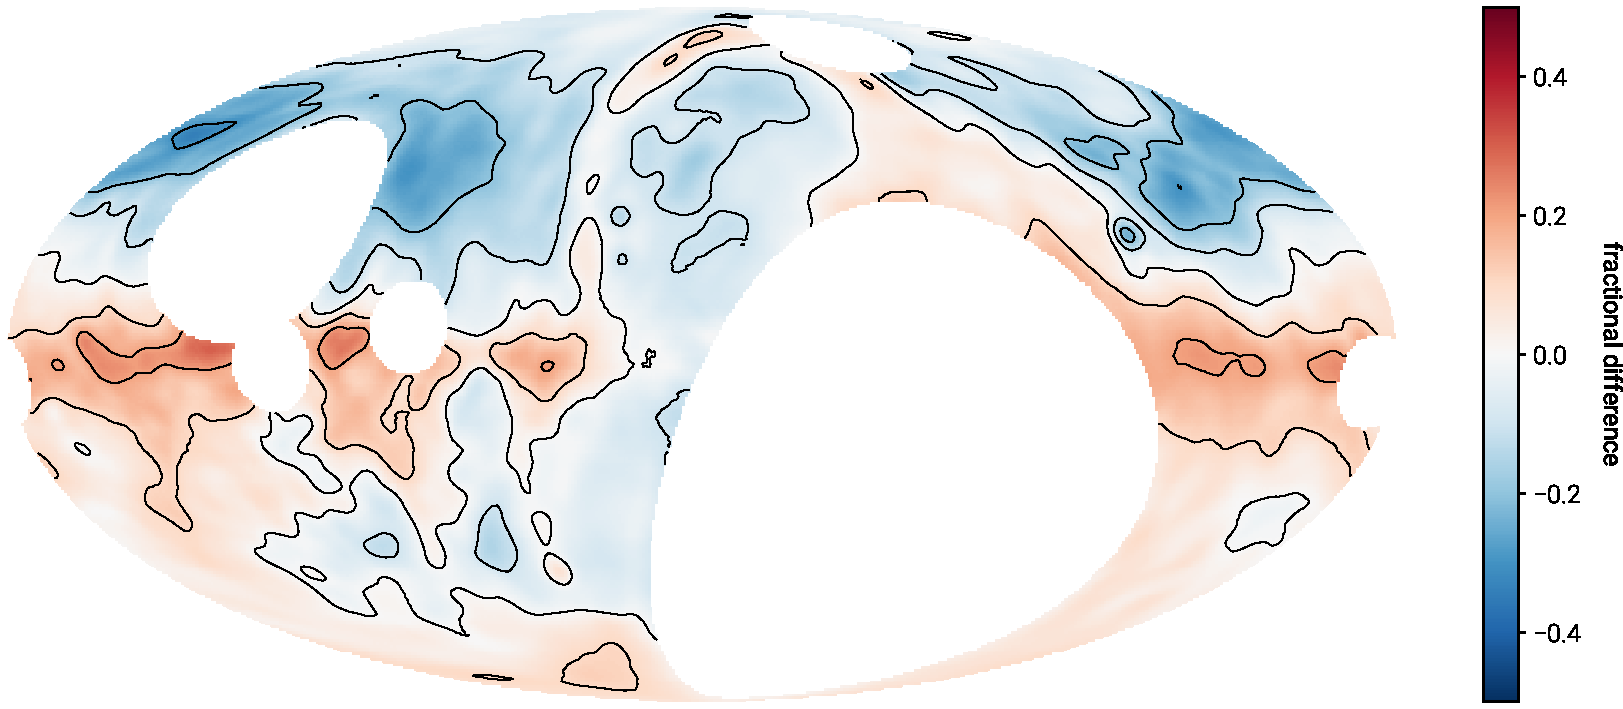
\includegraphics[height=0.32\textheight]{figures/chapter3/guzman}
    \caption{
        This Mollweide-projected map compares the fractional difference between the Guzm\'{a}n 45
        MHz map and the OVRO-LWA maps (Figure~\ref{fig:channel-maps}) interpolated to 45~MHz
        (degraded to $5^\circ$ resolution). A positive value indicates regions where the OVRO-LWA
        map has more emission than the Guzm\'{a}n map, and a negative value indicates regions where
        the Guzm\'{a}n map has more emission than the OVRO-LWA map. Cas A, Cyg A, Vir A, and Tau A
        are masked due to the fact that they are subtracted from the OVRO-LWA maps but not the
        Guzm\'{a}n map.
    }
    \label{fig:guzman-comparison}
\end{figure*}

The Guzm\'{a}n 45 MHz map \citep{2011A&A...525A.138G} is compiled from a southern hemisphere survey
\citep{1997A&AS..124..315A} and a northern hemisphere survey \citep{1999A&AS..140..145M}, with a
small gap around the NCP. In this work, the zero level is set by comparing against published
low-frequency measurements in six different directions.

A direct comparison between the OVRO-LWA maps interpolated to 45 MHz and the Guzm\'{a}n 45 MHz map
can be seen in Figure~\ref{fig:guzman-comparison}. In order to make this comparison, the OVRO-LWA
map was degraded to a 5$^\circ$ resolution by convolving with a Gaussian kernel, and the Guzm\'{a}n
map has had spherical harmonics with $m=0$ discarded in order to make it consistent with the maps
presented in this paper. This figure shows an $\sim20\%$ excess of emission in the galactic plane
that is consistent with the discrepancy observed between the LLFSS and the Guzm\'{a}n map.  However,
while the LLFSS has an excess of emission near the north galactic pole, no such excess is observed
in this work. Instead, there is a 10\% excess of emission near the south galactic pole. Elsewhere off
the plane of the galaxy, the discrepancy can be as much as $-20\%$.

\citet{2011A&A...525A.138G} computed the spectral index between their 45~MHz map and the 408~MHz
Haslam map. Along the galactic plane, the spectral index varies between -2.2 (in the vicinity of
\ion{H}{2} regions) and -2.5 (at galactic longitudes $\sim 180^\circ$). The north galactic spur has
a spectral index of -2.5. This is generally consistent with the results presented in
Figure~\ref{fig:haslam-spectral-index}.

%%%%%%%%%%%%%%%%%%%%%%%%%%%%%%%%%%%%%%%%%%%%%%%%%%%%%%%%%%%%%%%%%%%%%%%%%%%%%%%%%%%%%%%%%%%%%%%%%%%%
\section{Error Analysis}\label{sec:error}

\subsection{The Ionosphere}\label{sec:ionosphere}

\begin{figure*}[t]
    \centering
    \begin{tabular}{cc}
        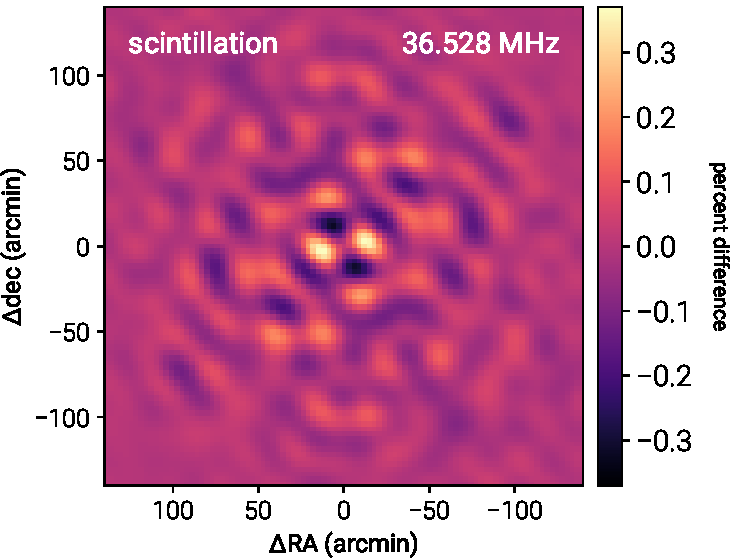
\includegraphics[width=\columnwidth]{figures/chapter3/scintillation-4} &
        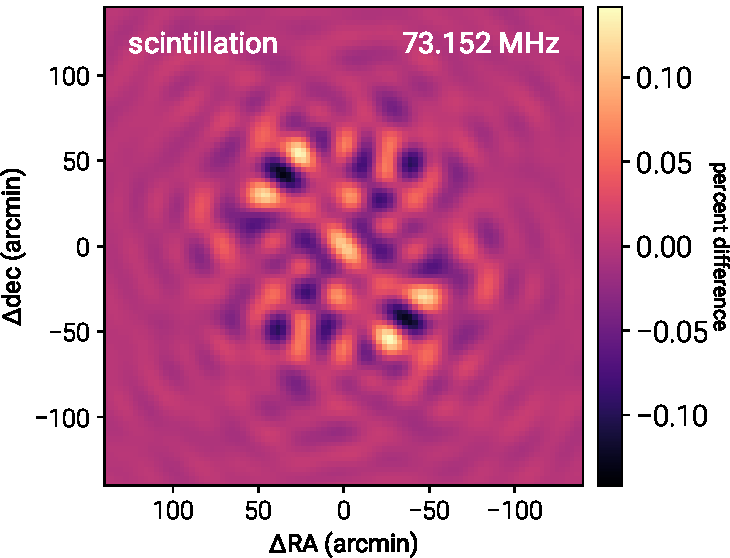
\includegraphics[width=\columnwidth]{figures/chapter3/scintillation-18} \\
        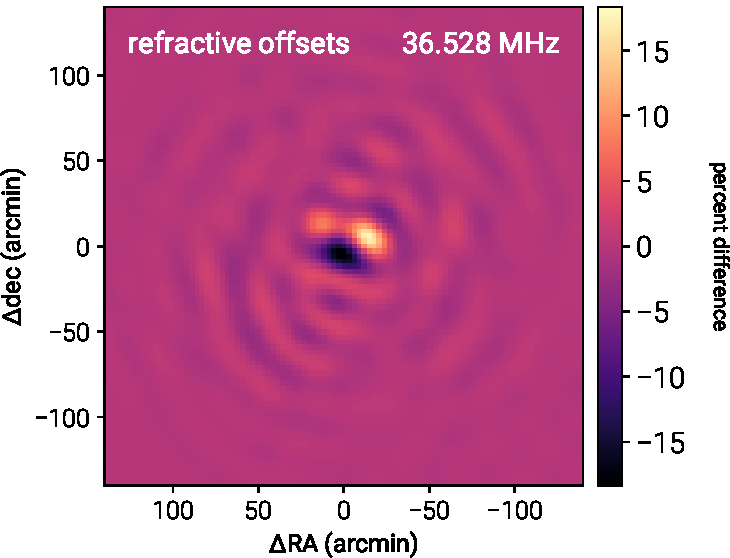
\includegraphics[width=\columnwidth]{figures/chapter3/refraction-4} &
        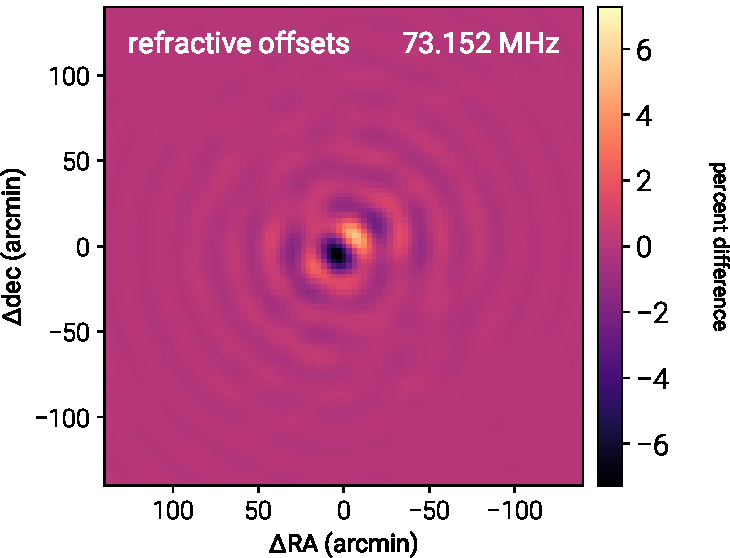
\includegraphics[width=\columnwidth]{figures/chapter3/refraction-18} \\
    \end{tabular}
    \caption{
        Illustration of the corrupting influence of the ionosphere at 36.528~MHz (left column)
        compared with 73.152~MHz (right column). Each panel shows the simulated PSF for a source at
        the location of Cas~A and illustrates the percent difference (relative to the peak flux of
        the uncorrupted PSF) due to including an ionospheric effect.  In the top row, the simulated
        source scintillates using the measured light curve for Cas~A in
        Figure~\ref{fig:scintillation}. In the bottom row, the simulated source is refracted from
        its true position using the measured refractive offsets for Cas~A in
        Figure~\ref{fig:scintillation}.
    }
    \label{fig:ionospheric-simulations}
\end{figure*}

\begin{figure*}[t]
    \centering
    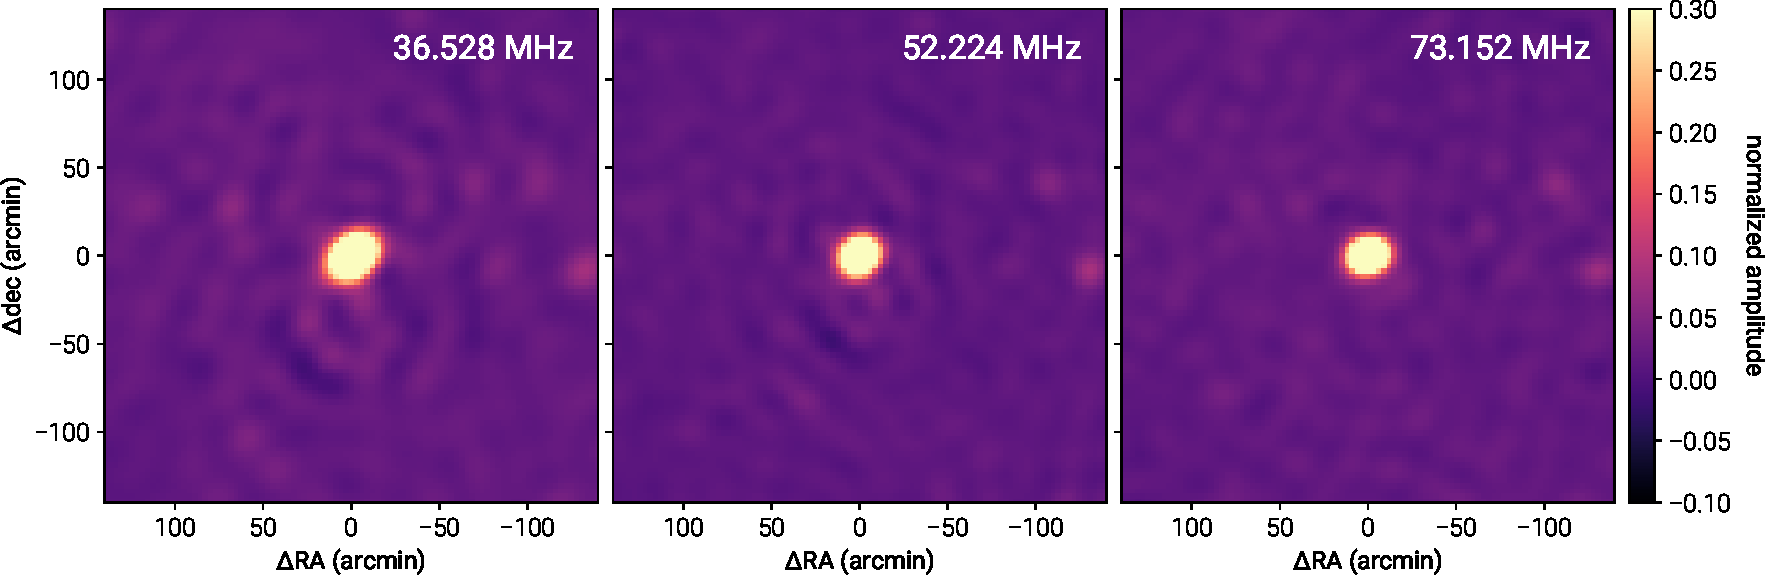
\includegraphics[width=\textwidth]{figures/chapter3/3C134}
    \caption{
        Zoom-in of 3C~134 at 36.528~MHz (left panel), 52.224~MHz (middle panel), and 73.152~MHz
        (right panel). At 36.528~MHz there are $\sim10\%$ artifacts around 3C~134 that persist after
        CLEANing due to ionospheric effects. As expected for an ionospheric origin, these artifacts
        decrease in amplitude as frequency increases. Figure~\ref{fig:ionospheric-simulations} shows
        the typically expected amplitude of these effects for ionospheric scintillation and
        refractive offsets.
    }
    \label{fig:3C134}
\end{figure*}

One of the key assumptions made by $m$-mode analysis is that the sky is static.  We assume that the
only time-dependent behavior is the rotation of the Earth, which slowly rotates the sky through the
fringe pattern of the interferometer. At low frequencies, the ionosphere violates this assumption.
In particular, ionospheric scintillation and refractive offsets will cause even static sources to
exhibit significant variability (Figure~\ref{fig:scintillation}).

The correlation observed on a given baseline for a single point source is
\begin{equation}
    V_\nu(t_{\textrm{sidereal}}) = I_\nu B_\nu(t_{\textrm{sidereal}}),
\end{equation}
where $I_\nu$ is the flux of the source at the frequency $\nu$, and $B_\nu$ is the baseline transfer
function defined by Equation~\ref{eq:baseline-transfer-function}. The transfer function is a
function of the direction to the source, which is in turn a function of the sidereal time
$t_{\textrm{sidereal}}$. If the source is varying, from intrinsic variability or due to
scintillation, then the source flux is also a function of the time coordinate $t$ such that
\begin{equation}
    V_\nu(t_{\textrm{sidereal}}) = I_\nu(t) B_\nu(t_{\textrm{sidereal}}),
\end{equation}
where $t_{\textrm{sidereal}} = (t \mod 23^h56^m)$.

In order to compute the $m$-modes, we must take the Fourier transform with respect to the sidereal
time. As a consequence of the Fourier convolution theorem, we find
\begin{equation}\label{eq:no-longer-block-diagonal}
    V_{\nu, m} \sim \sum_{m^\prime} V_{m^\prime}^\textrm{static} I_{\nu, m-m^\prime}\,,
\end{equation}
where $V_{\nu, m}^{\textrm{static}}$ is the set of observed $m$-modes if the source was actually
static, and $I_{\nu, m-m^\prime}$ is the Fourier transform of the light curve $I_{\nu}(t)$.
Equation~\ref{eq:no-longer-block-diagonal} indicates that power is scattered between different
values of $m$. As a consequence, the true transfer matrix, which is exactly block diagonal in the
ideal case, is no longer truly block diagonal \citep{richard_ionosphere_thoughts}.

The maps presented in Figure~\ref{fig:channel-maps} do not account for any off-diagonal terms
arising from ionospheric fluctuations. The effect of this can be seen in
Figure~\ref{fig:ionospheric-simulations}. In this simulation, a point source is placed at the
location of Cas~A. In one case, the source is allowed to scintillate in the same way Cas~A does in
Figure~\ref{fig:scintillation}, but the source is always located exactly at the location of Cas~A.
In the second case, the source position is allowed to vary in the same way Cas~A does in
Figure~\ref{fig:scintillation}, but the flux of the source exactly traces the beam model. The
scintillation, although large, introduces only $<0.3\%$ errors in the vicinity of bright point
sources. Refractive offsets, however, can introduce $\sim 15\%$ errors at 36.528~MHz and $\sim 5\%$
errors at 73.152~MHz.  Because the sidelobes of the PSF are altered from that of the ideal PSF,
refractive offsets will restrict the dynamic range it is possible to obtain with the CLEAN algorithm
described in \S\ref{sec:clean}. This effect can be clearly seen in Figure~\ref{fig:3C134}, where
10\% errors within 1$^\circ$ of 3C~134 are seen at 36.528~MHz.  As expected for an ionospheric
effect, these errors decrease to a few percent at 52.224~MHz, and less at 73.152~MHz. We therefore
conclude that ionospheric effects directly limit the dynamic range in the vicinity of bright point
sources.

\subsection{Beam Errors}

A model of the antenna beam is essential for wide-field imaging. Because $m$-mode analysis imaging
operates on a full sidereal day of data, images are constructed after watching each point in the sky
move through a large slice of the beam (excepting the celestial poles). The beam model therefore
serves two purposes:
\begin{enumerate}
    \item setting the flux scale as a function of declination and
    \item reconciling observations from two separate sidereal times.
\end{enumerate}

In the first case, all sources at a given declination take the same path through the antenna primary
beam. If the antenna response is overestimated along this track, then all sources at this
declination will have underestimated fluxes. Similarly, if the antenna response is underestimated,
then all the sources will have overestimated fluxes. The errors in Figure~\ref{fig:flux-scale} do
not show a clear pattern with declination. Two sources have a clear systematic offset at all
frequencies: 3C 353 and 3C 380. Source 3C 353 is the second southernmost source, but Hya A -- the
first southernmost source -- does not exhibit this systematic error. Similarly, 3C 380 is at a
comparable declination to Lyn A, which appears, if anything, to have its flux systematically offset
in the other direction. The absence of a coherent pattern does not eliminate the possibility of beam
errors affecting the flux scale, but it does mean that these errors are at least comparable to the
errors inherent to the flux scale itself.

The second case is more subtle. Sources are observed at a wide range of locations in the primary
beam of the antenna. The imaging process must reconcile all of these observations together, and the
beam model provides the instructions for how to do this. In the event of an error in the beam model,
it can be expected that the beam will introduce errors into the sky maps that will limit the dynamic
range in the vicinity of bright point sources.  \citet{2015PhRvD..91h3514S} simulated the effect of
beam errors on a cosmological analysis, concluding that the beam must be known to one part in $10^4$.
Our requirements are significantly less stringent because we are estimating the sky brightness
instead of estimating the amplitude of a faint cosmological signal in the presence of foreground
emission that dominates the signal by five orders of magnitude. In fact, in \S\ref{sec:ionosphere}
we found that ionospheric effects likely dominate over other sources of error that affect the PSF
shape. Therefore, we conclude that the beam models generated in \S\ref{sec:beam} are sufficient to
limit the effect of beam errors on the PSF to at least less than those introduced by the ionosphere.

\subsection{Polarization Leakage}

\citet{2015PhRvD..91h3514S} described how to generalize $m$-mode analysis to account for a polarized
sky observed with a polarized antenna beam. Heretofore, this generalization has been neglected in the
discussion of $m$-mode analysis imaging.  At low frequencies, increasingly rapid Faraday rotation
leads to depolarization. Therefore, polarization fractions are generally expected to decrease at low
frequencies (varying with ionospheric conditions). \citet{2016ApJ...830...38L} detected the presence
of diffuse polarized emission on degree angular scales with the MWA, also finding typical
depolarization ratios of $\sim0.3$ for pulsars at 154~MHz relative to 1.4~GHz, although there was a
large variance between pulsars. Even more depolarization is expected at frequencies $\le
73.152$~MHz, but crossed-dipole antennas with extremely large primary beams will naturally introduce
large polarization leakage terms at low elevations.  It is instructive to compute what impact this
will have on the unpolarized imaging process.

In order to understand the effect of polarization leakage, we simulated a point source with 10\%
polarization in Stokes $Q$ at the location of Cas A.  The simulated visibilities were computed using
the measured beams for the $x$ and $y$ dipoles. Because the amplitudes of the two beams are not equal in
every direction on the sky, this introduces a direction-dependent leakage of Stokes $Q$ into
Stokes $I$. At 73.152~MHz, this leakage is $\lesssim5\%$ above $15^\circ$ elevation but rapidly
rises to $\gtrsim50\%$ at lower elevations. \citet{2015JAI.....450004O} reported similar polarization
leakage measurements with the LWA1.  Cas A is a circumpolar source and spends about 7 hours
every day skirting the horizon where the polarization leakage is large, so by placing the simulated
source at the location of Cas A, we are engineering a situation where the polarization leakage from
Stokes $Q$ into Stokes $I$ will be large. However, the impact on the unpolarized $m$-mode analysis
maps is mild, amounting to a 0.5\% error in the flux of the source.

\subsection{Terrestrial Interference and Pickup}\label{sec:rfi}

\begin{figure*}[t]
    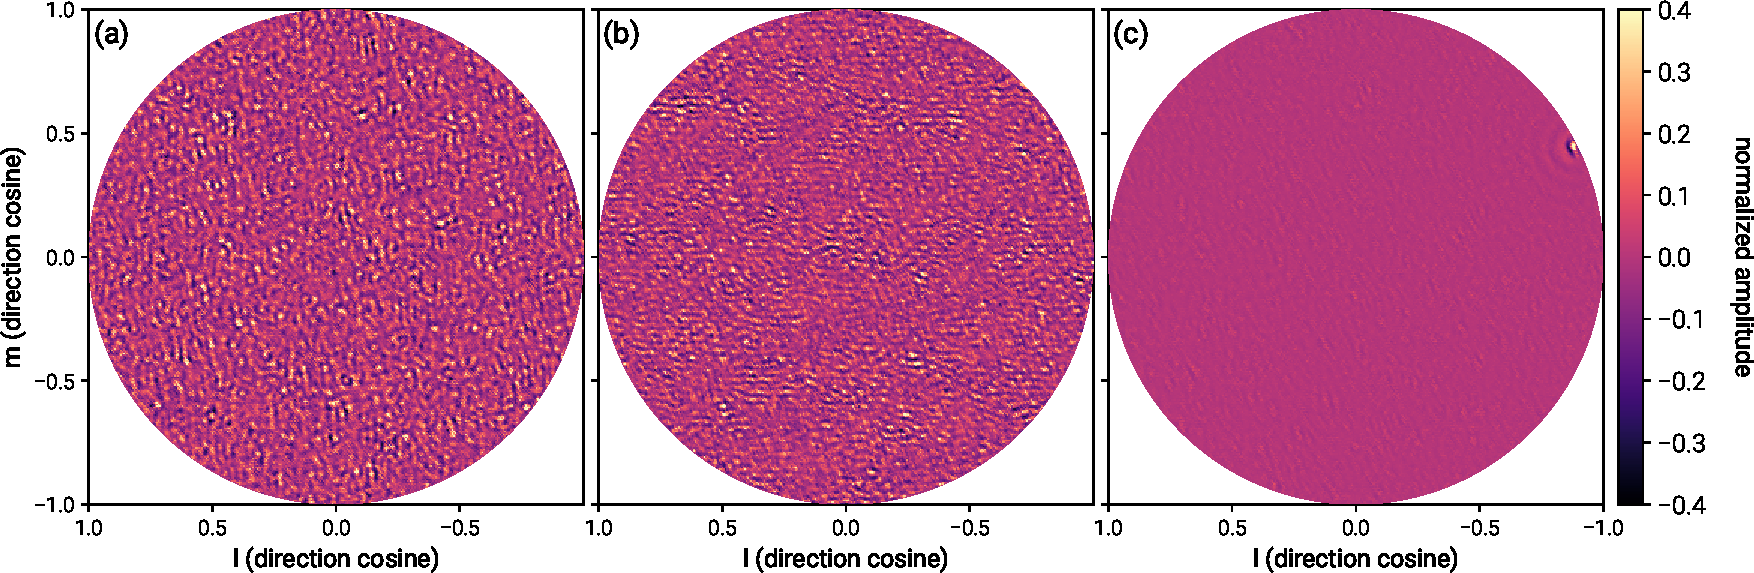
\includegraphics[width=\textwidth]{figures/chapter3/smeared}
    \caption{
        Terrestrial sources of correlated noise that are apparent after averaging the visibilities
        at 62.688~MHz over the entire 28 hour observing period (keeping the phase center at zenith
        such that astronomical sources of radio emission are smeared along tracks of constant
        declination). Each panel represents a different component that is removed from the
        visibilities. The images are generated using WSClean \citep{2014MNRAS.444..606O}, uniform
        weighting, and only baselines longer than 15 wavelengths. Panels (a) and (b) illustrate
        components that appear noise-like in image space, but are in fact a constant offset to the
        measured visibilities likely associated with cross-talk or common-mode pickup. Panel (c)
        illustrates a component that is clearly associated with an RFI source on the horizon to the
        west--northwest of the OVRO-LWA. This RFI source is likely an arcing power line.
        Figure~\ref{fig:rings} illustrates the characteristic ringlike artifacts introduced into the
        maps if these three components are not removed prior to $m$-mode analysis imaging. The
        component shown in panel (a) has about twice the amplitude ($\|\b v_\text{terrestrial}\|$)
        of those in panels (b) and (c), and for all three components, $\|\b B^*\b
        v_\text{terrestrial}\|/(\|\b B\|\|\b v_\text{terrestrial}\|) \sim 0.035$.
    }
    \label{fig:fitrfi}
\end{figure*}

\begin{figure*}[t]
    \centering
    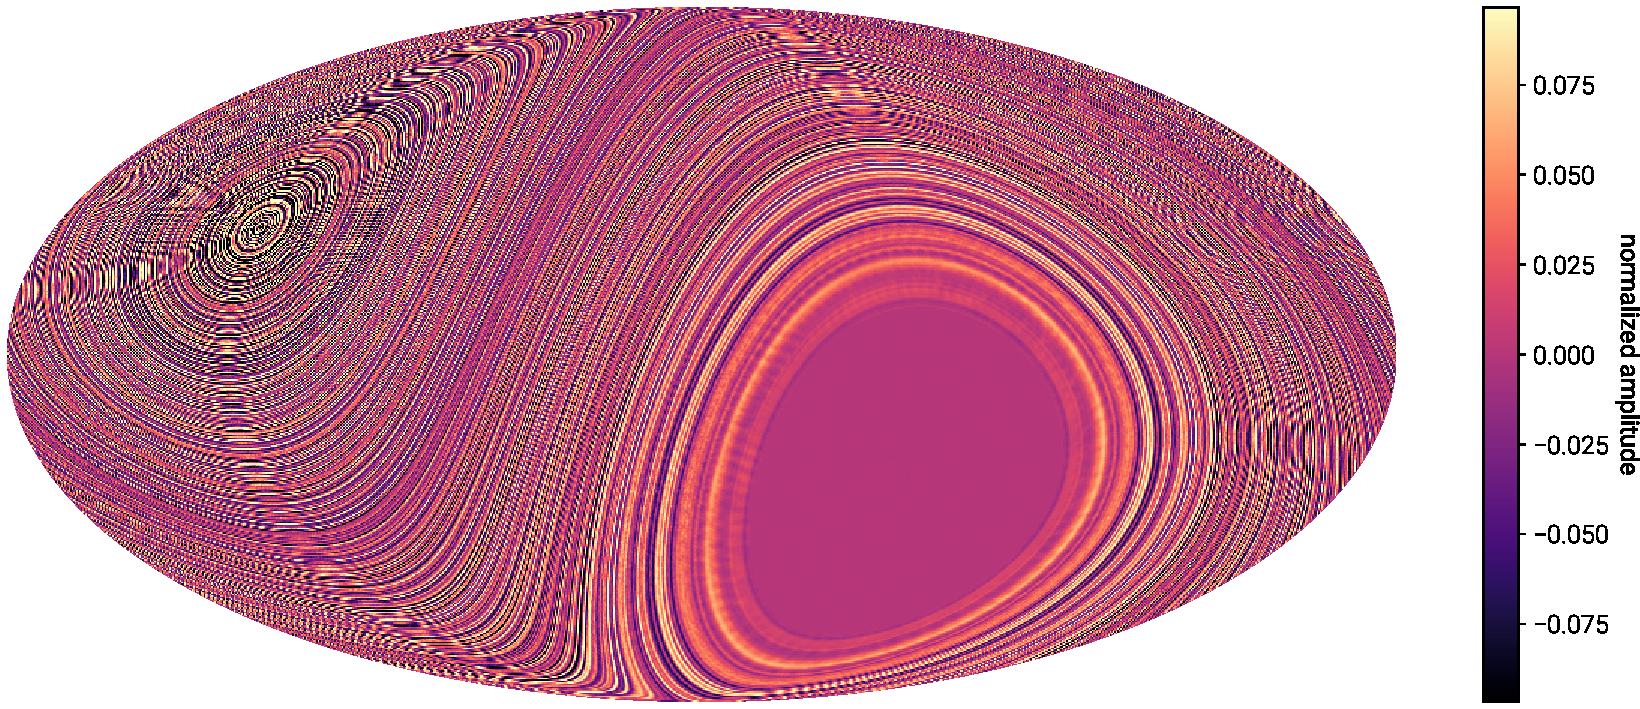
\includegraphics[height=0.32\textheight]{figures/chapter3/rings}
    \caption{
        A Mollweide-projected image of the artifacts introduced to the $m$-mode analysis maps by the
        three terrestrial sources shown in Figure~\ref{fig:fitrfi}. Because these sources are not
        moving through the sky sidereally, they tend to be smeared along rings of constant
        declination. The spurs seemingly radiating from the NCP are a Moir\'{e} pattern (i.e., an
        artifact of the pixelization).
    }
    \label{fig:rings}
\end{figure*}

When writing Equation~\ref{eq:basic-imaging}, it is implicitly assumed that the correlated voltage
fluctuations measured between pairs of antennas are exclusively generated by astronomical sources of
radio emission. In practice, this assumption can be violated. For instance, a low-frequency
interferometer located in the vicinity of an arcing power line will see an additional contribution
from the RFI generated by the arcing process. Similarly, common-mode
pickup along the analog signal path of the interferometer may generate an additional spurious
contribution to the measured visibilities. While the amplitude and phase of these contaminating
signals may fluctuate with time, they do not sweep across the sky at the sidereal rate
characteristic of astronomical sources.

The Owens Valley is an important source of water and power for the city of Los Angeles.
Unfortunately, this means that high-voltage power lines run along the valley $\gtrsim10$~km to the
west of the OVRO-LWA. Some of these power-line poles have faulty insulators that arc and produce
pulsed, broadband RFI. Because these poles exist in the near-field of the array, we have been able
to localize some of them by using the curvature of the incoming wavefront to infer a distance.
Efforts are currently underway to work with the utility pole owners to have these insulators
replaced.

In the meantime, it is possible to suppress their contamination in the data set. The contribution of
these RFI sources to the visibilities can be plainly seen by averaging $>24$ hours of data with the
phase center set to zenith. In this way, true sky components are smeared along tracks of constant
declination while terrestrial sources (i.e., the arcing power lines or any contribution due to
common-mode pickup) are not smeared.  Obtaining a model for the RFI is complicated by the fact that
the contaminating sources are at extremely low elevations, where the antenna response is essentially
unknown (and inhomogeneous due to antenna shadowing effects). It is not enough to know the physical
location of the faulty insulator generating the RFI. In addition, we must know the response of each
antenna (amplitude and phase) in the appropriate direction. This motivates the use of peeling, which
allows the antenna response to be a free parameter.  Therefore, model visibilities for the RFI can
be obtained by peeling the sources after smearing the visibilities over $>24$ hours.
Figure~\ref{fig:fitrfi} shows an illustration of some of the removed components at 62.688 MHz.

While attempting to peel RFI sources from the averaged visibilities, it was discovered that
frequently peeling would remove components from the visibilities that are not obviously associated
with any source on the horizon or elsewhere in the sky (see panels (a) and (b) in
Figure~\ref{fig:fitrfi}).  These components appear noise-like in the images, but they are actually a
constant offset to the measured visibilities and are therefore likely associated with cross-talk or
some form of common-mode pickup. If these components are not subtracted from the measured
visibilities, they contribute ringlike structures to the sky maps, as seen in
Figure~\ref{fig:rings}. This figure is not a simulation but rather a difference between maps created
before and after measuring and subtracting the components in Figure~\ref{fig:fitrfi} from each
integration.

The first step in Equation~\ref{eq:tikhonov-solution} is to compute $\b B^*\b v$. In this step, we
compute the projection of the measurement $\b v$ onto the space spanned by the columns of $\b B$.
Each column of $\b B$ describes the interferometer's response to a corresponding spherical harmonic
coefficient of the sky-brightness distribution. Therefore, the act of computing $\b B^*\b v$ is to
project the measured $m$-modes onto the space of $m$-modes that could be generated by astronomical
sources. The degree to which a source of terrestrial interference will contaminate a map generated
using $m$-mode analysis imaging is determined by its amplitude after projection.

For instance, a bright interfering source might contribute $\b v_\text{terrestrial}$ to the measured
$m$-modes. However, if $\b v_\text{terrestrial}$ is actually perpendicular to all of the columns of
$\b B$, there will be no contamination in the map because $\b B^*\b v_\text{terrestrial} = \b 0$.
In practice, this is unlikely. In general, the contamination is proportional to the overall amplitude
of the interference ($\|\b v_\text{terrestrial}\|$) and the degree to which the interference mimics
an astronomical signal ($\|\b B^*\b v_\text{terrestrial}\|/(\|\b B\|\|\b v_\text{terrestrial}\|)$).

These terrestrial sources do not rotate with the sky, and hence their contamination tends to be
restricted to modes with small $m$. In this data set the contamination is largely restricted to $m
\lesssim 1$. Although the RFI is capable of fluctuating on short timescales, in this case, the
artifacts it introduces seem to be restricted to small $m$ (presumably because the phase is not
fluctuating).  As a result, if the contamination is not suppressed, it will manifest itself as rings
along stripes of constant declination. This effect is plainly visible in Figure~\ref{fig:fitrfi}.
Because of the distinctive ringlike pattern created by terrestrial sources, we additionally chose to
discard spherical harmonics with either $m=0$ or $m=1$ and $l>100$ in order to further suppress the
contamination.

%%%%%%%%%%%%%%%%%%%%%%%%%%%%%%%%%%%%%%%%%%%%%%%%%%%%%%%%%%%%%%%%%%%%%%%%%%%%%%%%%%%%%%%%%%%%%%%%%%%%
\section{Conclusion}\label{sec:conclusion}

In this work, we presented a new imaging technique -- Tikhonov-regularized $m$-mode analysis imaging
and CLEANing -- for drift-scanning telescopes like the OVRO-LWA.  This technique exactly corrects
for wide-field effects in interferometric imaging with a single synthesis imaging step.  We applied
Tikhonov-regularized $m$-mode analysis imaging to a 28 hour data set and generated eight sky maps
between 36.528 and 73.152~MHz.  These sky maps are a substantial improvement in angular resolution
over existing maps at these frequencies with $\sim15\arcmin$ angular resolution and $<600$~K thermal
noise. The point-source flux scale is consistent with that defined by \citet{2012MNRAS.423L..30S} to
about 5\%, and large angular scales are consistent with the work of \citet{2017MNRAS.469.4537D} to
within 20\%.

At frequencies above $\sim55$~MHz, the angular resolution of these maps is limited by the selection
of $l_\text{max}=1000$. Future work will increase $l_\text{max}$ to remove this restriction, as well
as include more time and bandwidth to improve the thermal noise. The usage of nighttime-only data
can help mitigate dynamic range limitations from the ionosphere and also eliminate solar sidelobe
residuals. Observations could also be extended to slightly higher and lower frequencies ($\sim27$ to
$85$~MHz) to take advantage of the full frequency range of the OVRO-LWA. The higher frequencies are
particularly interesting in order to maximize the overlap with the MWA in the southern hemisphere,
which could be used to fill in the hole around the southern celestial pole.

These maps and future improvements are primarily intended to be used as part of a foreground
modeling and subtraction routine for 21~cm cosmology experiments. Each map will be made publicly
available on LAMBDA.

\acknowledgments
This work is dedicated to the memory of Professor Marjorie Corcoran, who was an influential mentor
to MWE.

This material is based in part upon work supported by the National Science Foundation under grants
AST-1654815 and AST-1212226. The OVRO-LWA project was initiated through the kind donation of Deborah
Castleman and Harold Rosen.

Part of this research was carried out at the Jet Propulsion Laboratory, California Institute of
Technology, under a contract with the National Aeronautics and Space Administration, including
partial funding through the President's and Director's Fund Program.

This work has benefited from open-source technology shared by the Collaboration for Astronomy Signal
Processing and Electronics Research (CASPER).  We thank the Xilinx University Program for donations;
NVIDIA for proprietary tools, discounts, and donations; and Digicom for collaboration on the
manufacture and testing of DSP processors.

We thank the Smithsonian Astrophysical Observatory Submillimeter Receiver Lab for the collaboration
of its members.

Development, adaptation, and operation of the LEDA real-time digital signal-processing systems at
OVRO-LWA have been supported in part by NSF grants AST/1106059, PHY/0835713, and OIA/1125087.

GBT, JD, and FKS acknowledge support from the National Science Foundation under grant AST-1139974.

\putbib[thesis]
\end{bibunit}


\cleartoevenpage

\myepigraph
{Look to my coming on the first light of the fifth day, at dawn look to the east.}
{Gandalf}

\chapter{The 21\,cm Power Spectrum from the Cosmic Dawn: First Results from the OVRO-LWA}
\label{chapter4}

\begin{bibunit}

\section*{Abstract}
%\begin{abstract}
    The 21\,cm transition of neutral hydrogen is opening an observational window into the cosmic
    dawn of the universe---the epoch of first star formation ($z\sim 20$). We use 28\,hr of data
    from the Owens Valley Radio Observatory Long Wavelength Array (OVRO-LWA) to place upper limits
    on the spatial power spectrum of 21\,cm emission at $z \approx 18.4$ ($\Delta_{21} \lesssim
    10^4\,\text{mK}$). In the process we demonstrate the first application of the double
    Karhunen-Lo\`{e}ve transform for foreground filtering, and diagnose the systematic errors that
    are currently limiting the measurement. We also provide an updated model for the angular power
    spectrum of low-frequency foreground emission measured from the northern hemisphere, which can
    be used to refine sensitivity forecasts for next-generation experiments.
%\end{abstract}

%%%%%%%%%%%%%%%%%%%%%%%%%%%%%%%%%%%%%%%%%%%%%%%%%%%%%%%%%%%%%%%%%%%%%%%%%%%%%%%%%%%%%%%%%%%%%%%%%%%%
\section{Introduction}\label{sec:introduction}

The Cosmic Dawn of star formation in the universe is one of the final unexplored epochs of the
universe. During this time (very roughly $25 \gtrsim z \gtrsim 15$) the first generation of stars
and galaxies formed and brought an end to the Dark Ages. Ly$\alpha$ emission from this early star
formation couples the excitation temperature of the 21\,cm hyperfine structure transition (i.e., the
spin temperature) to the local gas temperature of the Intergalactic Medium
\citep[IGM;][]{1952AJ.....57R..31W, 1958PIRE...46..240F}. This allows the highly-redshifted 21\,cm
transition to be used as a probe of the density, temperature, and ionization state of the IGM
\citep[e.g.,][]{2006PhR...433..181F, 2012RPPh...75h6901P}.

The first detection of high-redshift ($z\sim 17$) atomic hydrogen in the globally averaged sky
temperature was recently reported by the EDGES experiment at 78\,MHz \citep{2018Natur.555...67B}.
This measurement was remarkable for its extreme amplitude ($\sim 500\,\text{mK}$).  A plethora of
new ideas have been proposed to explain the amplitude of the absorption trough. These new theories
generally fall into two categories: those that invoke new physics to cool the IGM at a rate faster
than pure adiabatic cooling would otherwise allow \citep[e.g.,][]{2018Natur.555...71B,
2018PhRvL.121a1101F}, and those that posit a new radio background originating from $z\gtrsim 20$
\citep[e.g.][]{2018arXiv180301815E, 2018ApJ...858L...9D}. Distinguishing between these alternatives,
and confirming the existing measurement now motivates a number of experiments.

The LEDA \citep{2018MNRAS.478.4193P} and SARAS~2 \citep{2018ApJ...858...54S} experiments are in the
process of attempting to directly confirm the EDGES detection in the global sky temperature using
radiometric dipole antennas.  Notably, each of these experiments employ materially different antenna
designs, which will, in principle, help address concerns regarding the role of the antenna beam and
its potential to introduce spectral structure into the measurement. As noted by
\citet{2018Natur.555...67B}, these independent measurements with independent processing pipelines
will be an important verification of an exceptionally difficult measurement.  The primary observing
challenge faced by global-detection experiments---such as EDGES, LEDA, and SARAS~2---is controlling
systematic errors introduced by foreground radio emission, instrumental effects, and the interaction
between them. Although these experiments calibrate their antennas and electronics with great care,
they must rely on external models of the foreground radio emission to model many types of systematic
errors.

In contrast, interferometers generally have the ability to self-calibrate and build self-consistent
models for the sky emission \citep[e.g.,][]{2018AJ....156...32E}. However, interferometers are
generally not used to measure the globally averaged sky brightness \citep{2016ApJ...826..116V}, but
instead measure the three dimensional spatial power spectrum of the 21\,cm brightness temperature
fluctuations. The global average and the spatial power spectrum are both statistics of the same
field and therefore a measurement of the spatial power spectrum can also provide evidence to support
a reject a putative detection in the global average.  A detection of the spatial power spectrum will
provide independent constraints on the temperature of the IGM and the timing of early star and
galaxy formation \citep[e.g.,][]{2017MNRAS.472.2651G}.  Additionally, the spatial power spectrum
carries additional information about the scale of the brightness temperature fluctuations, which may
be used to constrain, for example, the amplitude of Lyman--Werner feedback
\citep{2013MNRAS.432.2909F} and the spectral hardness of early X-ray sources
\citep{2014MNRAS.437L..36F} that heat the IGM.

At lower redshifts corresponding to the Epoch of Reionization (EoR), constraints on the 21\,cm
spatial power spectrum have been published by the PAPER experiment \citep{2015ApJ...809...61A},
LOFAR \citep{2017ApJ...838...65P}, the MWA \citep{2016ApJ...833..102B}, and the GMRT
\citep{2013MNRAS.433..639P}. At redshifts corresponding to the cosmic dawn, this measurement has
only been previously attempted by \citet{2016MNRAS.460.4320E} using 6\,hr of data from the MWA.  The
under-construction HERA experiment will aim to place the most sensitive limits to date on the 21\,cm
brightness temperature spatial power spectrum from both the EoR and Cosmic Dawn due to its large
collecting area and design lessons inherited from the PAPER experiment \citep{2017PASP..129d5001D}.

In this paper we attempt to measure the spatial power spectrum of 21\,cm brightness temperature
fluctuations with the OVRO-LWA. In the process we model, derive, and (where appropriate) measure the
contribution of thermal noise, foreground emission, and the 21\,cm signal to the full covariance
matrix of the data. This is possible due to the application of $m$-mode analysis
\citep{2014ApJ...781...57S, 2015PhRvD..91h3514S}, which introduces sparsity into the covariance
matrices without which it would not be possible to store the full covariance matrix of the data.

In \S\ref{sec:observations} we describe the observations, the calibration strategy, and point source
removal routines used in this work. In \S\ref{sec:formalism} we will describe the $m$-mode analysis
formalism and a new strategy for compressing the representation of the transfer matrix.  In
\S\ref{sec:sensitivity} we derive, model, and measure the contribution of noise, foreground emission
and the cosmological 21\,cm signal to the full covariance matrix of the measured data.  These
covariance matrices are applied to filter the foreground emission in
\S\ref{sec:foreground-filtering}, where we also build physical intuition for the action of the
foreground filters derived by \citep{2014ApJ...781...57S, 2015PhRvD..91h3514S}.  These foreground
filters are applied to 28\,hr of data from the OVRO-LWA to estimate the 21\,cm power spectrum in
\S\ref{sec:results}, where we also analyze the limiting systematic errors in our measurement.
Finally, in \S\ref{sec:conclusion} we present our conclusions.  Unless state otherwise, we adopt the
set of cosmological parameters measured by \citet{2016A&A...594A..13P}.

%%%%%%%%%%%%%%%%%%%%%%%%%%%%%%%%%%%%%%%%%%%%%%%%%%%%%%%%%%%%%%%%%%%%%%%%%%%%%%%%%%%%%%%%%%%%%%%%%%%%
\section{Observations}\label{sec:observations}

\begin{figure}[p]
    \centering
    \begin{tikzpicture}[node distance=1cm, font=\relsize{-1}]
        % nodes

        \node [base] (antenna) {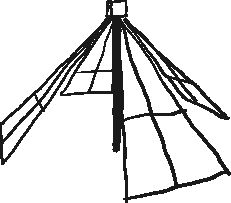
\includegraphics[width=2cm]{figures/chapter4/ovro-lwa-antenna}};
        \node [data, below=of antenna]       (raw)        {raw visibilities};
        \node [process, below=of raw]        (calibrate)  {direction-independent calibration};
        \node [process, below=of calibrate]  (stationary) {stationary component removal};
        \node [process, below=of stationary] (peeling)    {point source subtraction and peeling};
        \node [process, below=of peeling]    (fourier)    {Fourier transform};
        \node [data, below=of fourier]       (mmodes)     {$m$-modes ($\b v$)};

        \node [data, right=of raw]      (transfer) {transfer matrix ($\b B$)};

        \node [data, above=of transfer] (beam1) {};
        \node [data] (beam2) at ($ (beam1) + (-1cm:-0.1cm) $) {};
        \node [data] (beam3) at ($ (beam2) + (-1cm:-0.1cm) $) {
            beam model, $(u, v, w)$-coordinates, bandpass
        };

        \node [data, right=of beam1] (sky-model1) {};
        \node [data] (sky-model2) at ($ (sky-model1) + (-1cm:-0.1cm) $) {};
        \node [data] (sky-model3) at ($ (sky-model2) + (-1cm:-0.1cm) $) {
            foreground model,\\signal model,\\noise model
        };

        \node [data, below=of sky-model1] (covariance)
            {covariance matrices ($\b C_\text{21}$, $\b C_\text{fg}$, $\b C_\text{noise}$)};

        \node [data, below=of transfer] (compressed-transfer)
            {compressed transfer matrix\\$\b B\leftarrow\b R^*\b B$};
        \node [process, right=of compressed-transfer] (svd) {singular value decomposition};
        \node [data, right=of svd] (compressed-covariance)
            {compressed covariance matrices\\$\b C\leftarrow\b R^*\b C\b R$};

        \node [data, below=of compressed-transfer] (filtered-transfer)
            {foreground-filtered transfer matrix\\$\b B\leftarrow\b L^*\b B$};
        \node [process, right=of filtered-transfer] (kltransform1) {Karhunen-Lo\`{e}ve transform};
        \node [data, right=of kltransform1] (filtered-covariance)
            {foreground-filtered covariance matrices\\$\b C\leftarrow\b L^*\b C\b L$};

        \node [data, below=of filtered-transfer] (whitened-transfer)
            {noise-whitened transfer matrix\\$\b B\leftarrow\b W^*\b B$};
        \node [process, right=of whitened-transfer] (kltransform2) {Karhunen-Lo\`{e}ve transform};
        \node [data, right=of kltransform2] (whitened-covariance)
            {noise-whitened covariance matrices\\$\b C\leftarrow\b W^*\b C\b W$};

        \node [process, below=of kltransform2] (qestimator) {quadratic estimator};
        \node [data, left=of qestimator] (filtered-mmodes)
            {foreground-filtered $m$-modes\\$\b v\leftarrow\b W^*\b L^*\b R^*\b v$};
        \node [data, right=of qestimator] (ps)
            {21\,cm power spectrum estimate ($p_\alpha$)};

        \node [process, below=of qestimator] (tikhonov)
            {Tikhonov regularized imaging};
        \node [base, right=of tikhonov] (maps)
            {
                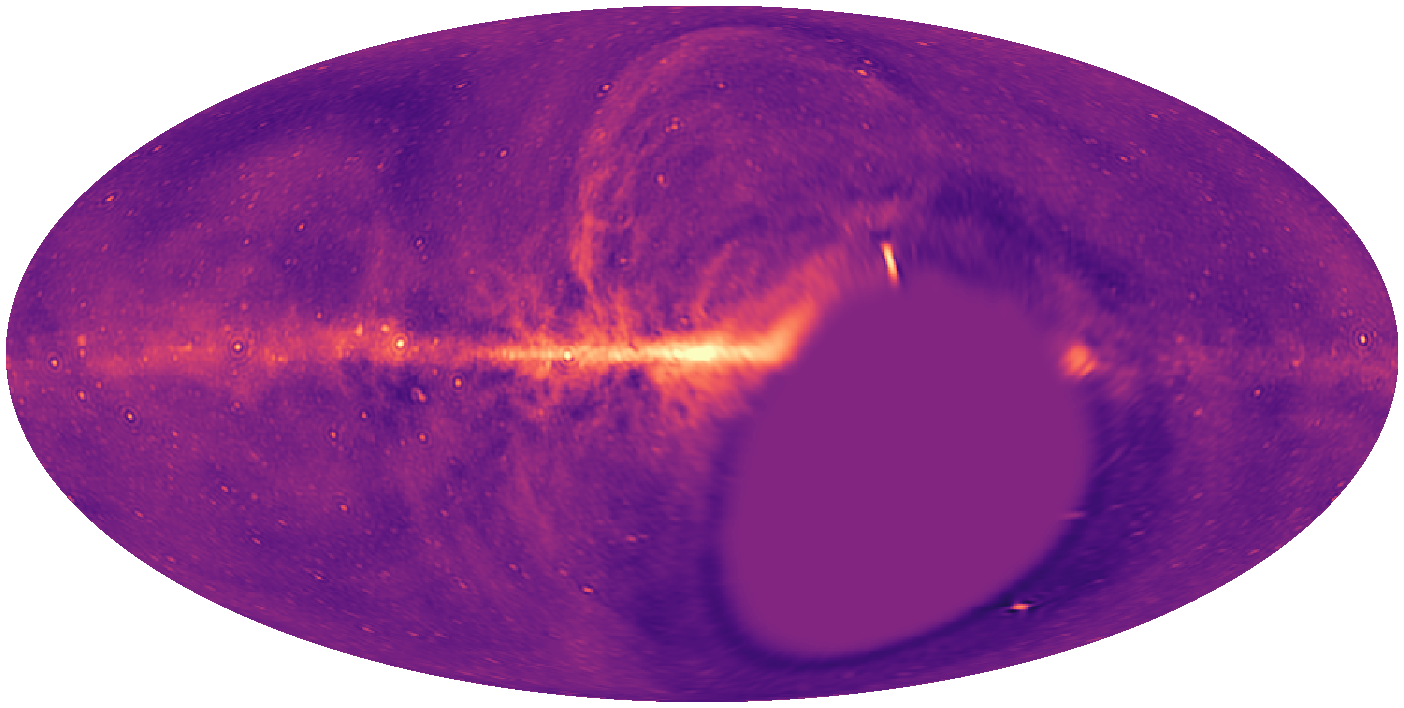
\includegraphics[width=3cm]{figures/chapter4/peeled-sky-map}
            };

        \node [rectangle, above left=-3.5mm and 1cm of tikhonov, rounded corners,
               draw, semithick, minimum width=7mm, minimum height=7mm] (B) {$\b B$};

        \coordinate [below left=+4mm and 4mm of mmodes] (corner);

        % edges

        \path [arrow-dashed] (antenna) -- (raw);
        \path [arrow] (raw) -- (calibrate);
        \path [arrow] (calibrate) -- (stationary);
        \path [arrow] (stationary) -- (peeling);
        \path [arrow] (peeling) -- (fourier);
        \path [arrow] (fourier) -- (mmodes);

        \path [arrow] (beam1) -- (transfer);
        \path [arrow] (transfer.south) to[|-|] (svd.140);
        \path [arrow] (svd) -- (compressed-transfer);
        \path [arrow] (compressed-transfer.south) to[|-|] (kltransform1.140);
        \path [arrow] (kltransform1) -- (filtered-transfer);
        \path [arrow] (filtered-transfer.south) to[|-|] (kltransform2.140);
        \path [arrow] (kltransform2) -- (whitened-transfer);

        \path [arrow] (sky-model1) -- (covariance);
        \path [arrow] (covariance.320) to[|-|] (svd.40);
        \path [arrow] (svd) -- (compressed-covariance);
        \path [arrow] (compressed-covariance.south) to[|-|] (kltransform1.40);
        \path [arrow] (kltransform1) -- (filtered-covariance);
        \path [arrow] (filtered-covariance.south) to[|-|] (kltransform2.40);
        \path [arrow] (kltransform2) -- (whitened-covariance);

        \path [arrow] (whitened-transfer.south) to[|-|] (qestimator.140);
        \path [arrow] (whitened-covariance.south) to[|-|] (qestimator.40);
        \path [arrow] (mmodes.10) -| (filtered-mmodes.south);
        \path [arrow] (filtered-mmodes) -- (qestimator);
        \path [arrow] (qestimator) -- (ps);

        \path [arrow] (mmodes.350) -- (tikhonov.190);
        \path [arrow] (B.east) to[-|-] (tikhonov.170);
        \path [arrow] (tikhonov) -- (maps);

        \path [line] (maps) |- (corner);
        \path [arrow] (corner) |- (calibrate);

    \end{tikzpicture}
    \caption{
        A flow chart describing the data analysis steps performed in this paper. Radio waves are
        received by antennas (depicted in the upper-left corner), which are correlated to produce
        raw visibilities. These visibilities are then flagged, calibrated, and bright point sources
        are removed. After a full sidereal day's worth of data has been collected, these
        visibilities can be Fourier transformed to compute the measured $m$-modes. Separately, an
        empirical beam model is used to calculate the transfer matrix elements that describe the
        interferometer's sensitivity to the sky. Full covariance matrices are computed for the
        foreground emission, 21\,cm signal, and thermal noise. These matrices are used to compress,
        filter foreground emission, and whiten the noise covariance. Finally, the resulting filtered
        $m$-modes are used to estimate the spatial power spectrum of 21\,cm emission. Images of the
        sky can be constructed through the use of Tikhonov-regularized imaging
        \citep{2018AJ....156...32E}, which are useful for diagnosing errors in the analysis.
    }
    \label{fig:flowchart}
\end{figure}

We collected 28\,hr of continuous data using the OVRO-LWA beginning at 2017 February 17 12:00:00
UTC. The OVRO-LWA is a low-frequency radio interferometer with a bandpass covering 27--85\,MHz ($50
\gtrsim z \gtrsim 16$), and is currently composed of 288 dual-polarization dipole antennas.  251 of
these antennas are arranged within a dense 200\,m diameter core in a configuration optimized for
sidelobe levels in snapshot images.  32 additional expansion antennas are placed outside of the
core, expanding the maximum baseline length to 1.5\,km. The remaining five antennas are equipped
with radiometric front-ends for total power measurements of the sky as part of the Large-Aperture
Experiment to Detect the Dark Ages \citep[LEDA;][]{2018MNRAS.478.4193P}.  The LEDA correlator serves
as the back-end for the OVRO-LWA, and cross-correlates 512 inputs with 58\,MHz instantaneous
bandwidth.  In this configuration the OVRO-LWA performs full cross-correlation of 256 antennas (512
signal paths), and 32 antennas (64 signal paths) are unused.  We selected the correlator's
integration time to be 13\,s due to the fact that this selection evenly divides the sidereal day to
within 0.1\,s.  In snapshot images, the OVRO-LWA can capture the entire visible hemisphere at
$10\arcmin$ resolution \citep[e.g.,][]{2017arXiv171106665A}, and this same dataset was used to
generate maps of the sky north of $\delta=-30\arcdeg$ \citep{2018AJ....156...32E}.

At low radio frequencies, propagation effects through the ionosphere are important.  During this
observing period, however, geomagnetic and ionospheric conditions were mild. At 73\,MHz, bright
point sources were observed to refract by up to $4\arcmin$ as waves propagated through the line of
sight on. Similarly at 73\,MHz, the apparent flux of point sources varied by up to 10\% on 13\,s
timescales due to ionospheric conditions.

In this work we selected data from an instrumental subband centered at 73.152\,MHz with 2.6\,MHz
bandwidth ($z=18.4$, $\Delta z=0.8$). This subband is contained within the absorption feature
observed by \citet{2018Natur.555...67B}, and contains the 73.0--74.6\,MHz band allocated for radio
astronomy in the United States. There is additionally a gap in television broadcasting between
72\,MHz (the upper edge of channel 4) and 76\,MHz (the lower edge of channel 5) that this observing
band takes advantage of.  Additionally, in previous work we published an updated low-frequency sky
map at 73.152\,MHz \citep{2018AJ....156...32E} that is available online at the Legacy Archive for
Microwave Background Data Analysis (LAMBDA).

When measuring the power spectrum of 21\,cm fluctuations, it is common to make an implicit
assumption that 21\,cm power spectrum is not evolving along the line-of-sight direction (see
Appendix~\ref{app:spatial-to-angular}).  \citet{2018MNRAS.477.3217G} simulated this effect and found
that for volumes of equal comoving radial distance, this light-cone effect is more severe during the
Cosmic Dawn than during the EoR.  Near $z \sim 18$ and a volume with $\Delta z \sim 3$, the
recovered spatial power spectrum is suppressed by a factor $\lesssim 2$. While the light-cone effect
can limit the usable bandwidth for estimating the 21\,cm spatial power spectrum, we conclude that
2.6\,MHz of bandwidth is permissible for this initial analysis. Future studies of 21\,cm
fluctuations of the Cosmic Dawn, however, should instead consider estimating the multi-frequency
angular power spectrum \citep{2007MNRAS.378..119D}, which is a statistic that is less common in the
literature, but can be measured without assuming that the statistics of the fluctuations are not
evolving along the line of sight.

A summary of the analysis steps performed in this work---including the instrumental calibration and
21\,cm power spectrum reduction---can be seen in Figure~\ref{fig:flowchart}.  In particular, a gain
calibration was derived from a 45\,minute track of data beginning at 2017 February 17 17:46:28
during which the two brightest point sources in the northern hemisphere (Cyg~A and Cas~A) are near
the meridian. The sky model is initially composed of Cyg~A and Cas~A where the absolute spectrum of
Cyg~A is given by \citet{1977A&A....61...99B}, and the spectrum of Cas~A is adjusted for its secular
decrease of 0.77\% per year \citep{2009AJ....138..838H}. Because this initial sky model is
incomplete on large angular scales, baselines shorter than 15 wavelengths are excluded from the
calibration routine.  The gains are optimized using a variant of alternating least squares
independently described by \citet{2008ISTSP...2..707M} and \citet{2014A&A...571A..97S}.  The
bandpass amplitude is fit with a 5th order polynomial, and the phase is fit with a term for the
delay and a term for dispersion through the ionosphere. Smoothing the gain calibration in this way
helps to avoid modeling errors during calibration propagating into bandpass errors that can limit
the sensitivity of the interferometer to the 21\,cm power spectrum \citep{2016MNRAS.461.3135B,
2017MNRAS.470.1849E}. After this initial calibration and source removal, a model of the diffuse
galactic emission is constructed using Tikhonov-regularized $m$-mode analysis imaging. This model is
then used to recalibrate the data with a more complete model of the sky.

The OVRO-LWA analog signal path is susceptible to additive common-mode radio frequency interference
(RFI). A model for the common-mode RFI is constructed from the gain-calibrated visibilities after
averaging over the entire 28\,hr observing period with the phase center left at zenith. Averaging
the visibilities in this way smears out the contribution of the sky along characteristic sidereal
tracks. We then select the dominant components of the averaged visibilities to be used as templates
for the RFI. The templates are manually inspected for residual sky emission by imaging each
component with WSCLEAN \citep{2014MNRAS.444..606O}, and checking for features that are swept along
sidereal tracks. These templates are scaled and subtracted from each integration to suppress the
contamination of the common-mode RFI.

The top panel of Figure~\ref{fig:before-after-source-removal-sky-maps} is a dirty image of the sky
constructed from this dataset prior to any point source removal.  A handful of bright point sources
occupy the northern sky---namely Cas~A, Cyg~A, Her~A, Hya~A, Tau~A, Vir~A, 3C~123, 3C~353, and the
Sun.  Each of these sources is removed from the visibilities employing a combination of
direction-dependent calibration for the brightest sources, and source fitting and subtraction for
the fainter sources. This source removal strategy is described in greater detail by
\citet{2018AJ....156...32E}.

Finally, in order to reduce the data volume and computational cost of further reductions, we
selected only baselines representable with spherical harmonics with multipole number $l \le 300$.
This effectively selects only baselines from the core of the OVRO-LWA, which contains the majority
of the brightness temperature sensitivity. The data was additionally averaged down to channel widths
of 240\,kHz. At 73\,MHz, this averaging effectively smears out the spatial power spectrum on
$k_\parallel \approx 1\,\text{Mpc}^{-1}$ scales, but is permissible because the expected
cosmological signal is small on these scales.

%%%%%%%%%%%%%%%%%%%%%%%%%%%%%%%%%%%%%%%%%%%%%%%%%%%%%%%%%%%%%%%%%%%%%%%%%%%%%%%%%%%%%%%%%%%%%%%%%%%%
\section{Formalism}\label{sec:formalism}

\subsection{$m$-Mode Analysis}

\begin{figure}
    \centering
    \begin{tabular}{c}
        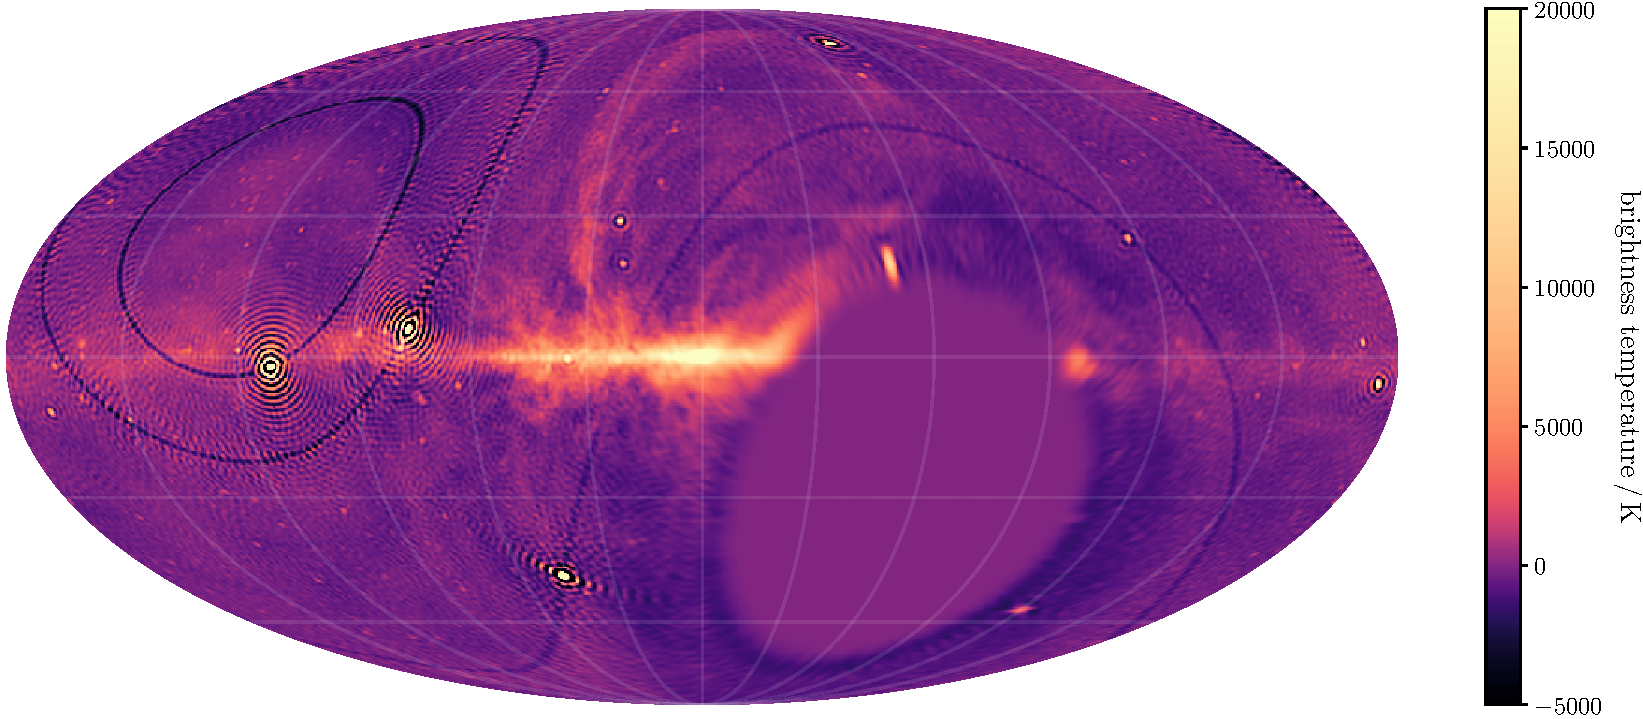
\includegraphics[width=\textwidth]{figures/chapter4/sky-map-colorbar} \\
        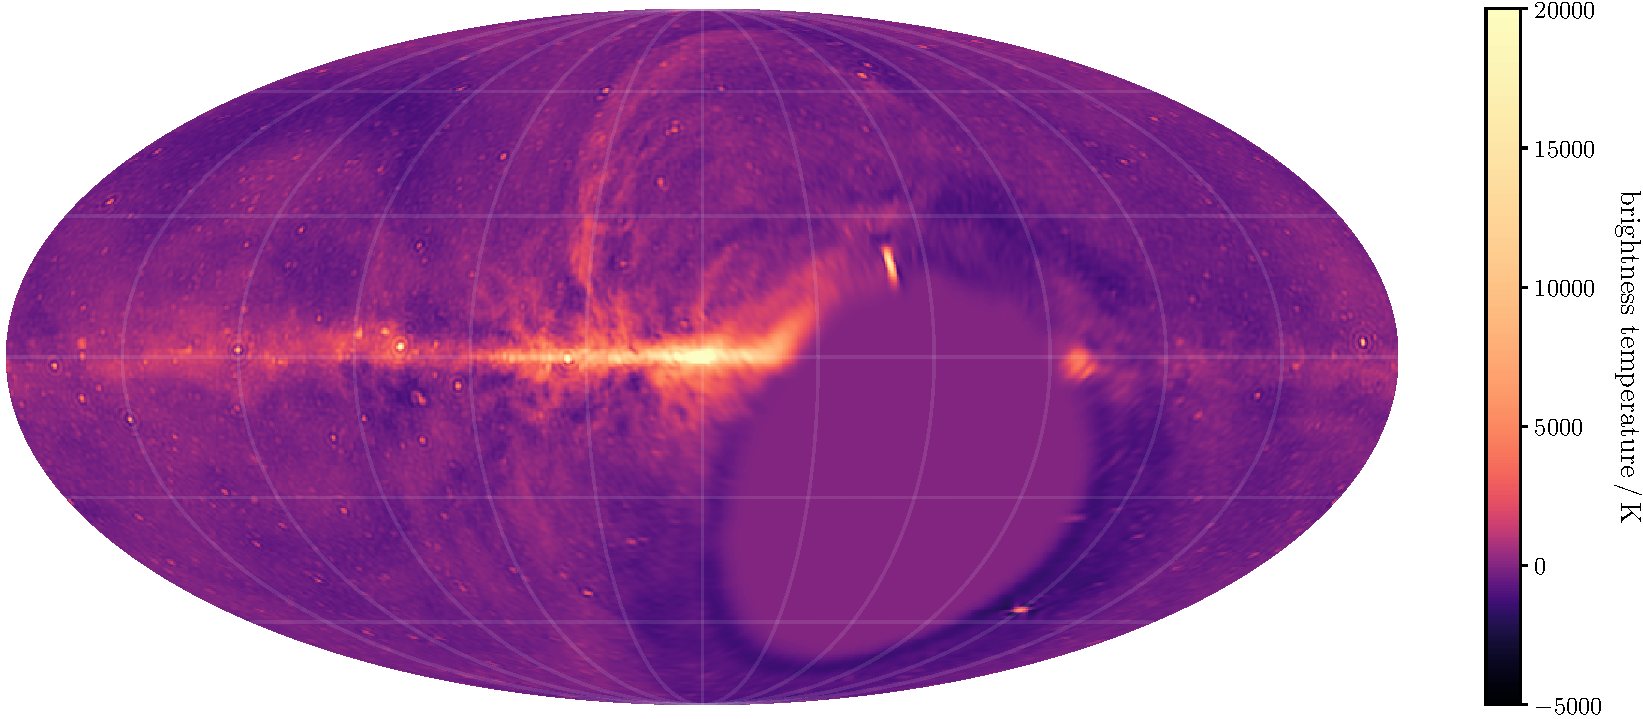
\includegraphics[width=\textwidth]{figures/chapter4/peeled-sky-map-colorbar} \\
    \end{tabular}
    \caption{
        A Molleweide projection of a Tikhonov-regularized image of the sky constructed from all
        baselines representable with $l_\text{max} \le 200$, and 2.6~MHz of bandwidth centered on
        73.2~MHz. The color scale is linear between $-1000$~K and $+1000$~K, and logarithmic outside
        of this range. No cleaning has been performed, so all point sources are convolved with a
        point spread function, and no masking of low declinations has been performed. The resolution
        of the maps naturally degrades at low declinations and the regularization scheme naturally
        encourages the map to be zero below the horizon. Negative rings at the declination of bright
        point sources are an artifact of the fact that $m=0$ modes are filtered from the dataset due
        to their susceptibility to RFI and common-mode pickup. (top) Before bright point sources are
        removed from the dataset. (bottom) After point source removal.
    }
    \label{fig:before-after-source-removal-sky-maps}
\end{figure}

In this paper we apply the $m$-mode analysis formalism developed by \citet{2014ApJ...781...57S,
2015PhRvD..91h3514S}. The interested reader should consult the aforementioned citations for
additional details, but $m$-mode analysis is briefly summarized below.

The measured quantity in a drift-scanning telescope is a periodic function of the sidereal time.
The Fourier transform with respect to sidereal time of this measured quantity is called an $m$-mode,
where the value of $m$ indicates how rapidly this mode varies over the course of a sidereal day.
$m=0$ corresponds to the mean value of the measurement over a sidereal day. $m=\pm1$ corresponds to
the components that varies once over a sidereal day. Larger absolute values of $m$ represent
contributions to the measurement that vary on increasingly rapid timescales.

The primary advantage of making this transformation to $m$-modes is that it can be shown that the
set of measured $m$-modes with a given value for $m$, are a linear combination of the spherical
harmonic coefficients with the same value of $m$. This allows the data to be partitioned by $m$, and
each partition can be manipulated independently of the remaining dataset. Typically this leads to a
large reduction in the processing time, which allows for the application of otherwise infeasible
data analysis techniques that make use of the full covariance matrix of the dataset.

We will adopt the convention that the measured $m$-modes are contained in a vector $\b v$, and the
spherical harmonic coefficients of the sky brightness are contained in a vector $\b a$. The transfer
matrix $\b B$ describes the interferometer's response to the sky and is block-diagonal when both $\b
v$ and $\b a$ are sorted by the absolute value of $m$. If we explicitly decompose the sky in terms
of the high-redshift 21\,cm contribution $\b a_\text{21}$, and the foreground radio emission $\b
a_\text{fg}$, then
\begin{equation}\label{eq:basic-m-mode-analysis}
    \b v = \b B \b a_\text{21} + \b B \b a_\text{fg} + \b n \,,
\end{equation}
where $\b n$ is the contribution of thermal noise to the measurement.

The rows of the transfer matrix $\b B$ fundamentally describe the response of each baseline to the
sky represented by $\b a$. The individual elements of the matrix are computed from spherical
harmonic transforms of each baseline's fringe pattern (including the response of the antenna beams
and bandpass). \citet{2018AJ....156...32E} demonstrated all-sky imaging in a single synthesis
imaging step through inverting Equation~\ref{eq:basic-m-mode-analysis}. However, that demonstration
was restricted to single channel imaging due to---in part---the computational and storage
requirements associated with computing $\b B$.

\subsection{Hierarchical Transfer Matrices}

Modern interferometers are composed of large numbers of antennas ($N \gg 10$) arranged in
configurations that have both long and short baselines. For instance, the OVRO-LWA has over 30,000
baselines. The shortest baseline is 5\,m, and the longest baseline is 1.5\,km. Consequently the
OVRO-LWA measures a large range of angular scales. We can exploit this fact to reduce the computer
time and disk space required to compute and store the transfer matrix $\b B$.

The sensitivity of a baseline of length $b$ to spherical harmonic coefficients with multipole moment
$l$ is $\propto j_l(2\pi b/\lambda)$, where $j_l$ is the spherical Bessel function of the first
kind, and $\lambda$ is the wavelength. When $l \gtrsim 2\pi b/\lambda$, the spherical Bessel
functions rapidly drop to zero (see Appendix~\ref{app:spatial-to-angular} for more details about
spherical Bessel functions). Consequently, even though the transfer matrix is block-diagonal, each
diagonal block of the transfer matrix can also contain a large number of zero-elements.

Therefore, when the columns and rows of each transfer matrix block $\b B_m$ are sorted by the
multipole number $l$ and baseline length respectively, each block has the following structure:
\begin{equation}
    \b B_m = \left(
        \quad
        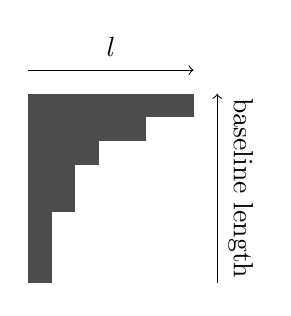
\begin{tikzpicture}[baseline=+13mm, scale=0.3]
            \draw [->] (0, 9) -- (7, 9);
            \node at (3.5, 10) {$l$};
            \draw [->] (8, 0) -- (8, 8);
            \node [rotate=270] at (9, 4) {baseline length};
            \fill [fill=black!70] (0, 0) rectangle (1, 1);
            \fill [fill=black!70] (0, 1) rectangle (1, 2);
            \fill [fill=black!70] (0, 2) rectangle (1, 3);
            \fill [fill=black!70] (0, 3) rectangle (2, 4);
            \fill [fill=black!70] (0, 4) rectangle (2, 5);
            \fill [fill=black!70] (0, 5) rectangle (3, 6);
            \fill [fill=black!70] (0, 6) rectangle (5, 7);
            \fill [fill=black!70] (0, 7) rectangle (7, 8);
        \end{tikzpicture}
        \quad
    \right)
\end{equation}
Shaded regions represent elements with nonzero value, whereas unshaded regions represent elements
with approximately zero value due to the fact that $l \gtrsim 2\pi b/\lambda$. This structure makes
it apparent that it is not necessary to store every element of each transfer matrix block. In fact,
by partitioning the array into sets of baselines with similar length, one can achieve significant
cost savings when computing and storing the transfer matrix elements.

Ultimately, for the OVRO-LWA we achieve a 58\% compression of the transfer matrix by not storing
elements that are approximately zero.

\subsection{Data Compression}\label{sec:compression}

Further data compression is desirable because it reduces the computational costs of all following
analysis steps. We implement the singular value decomposition (SVD) compression described by
\citep{2014ApJ...781...57S, 2015PhRvD..91h3514S}. The SVD factorizes a matrix into a unitary matrix
$\b U$, a diagonal matrix $\b\Sigma$, and another unitary matrix $\b V$ such that
\begin{equation}
    \b B = \b U \b\Sigma \b V^*\,.
\end{equation}
The diagonal elements of $\b\Sigma$ are called singular values and, in this case, represent the
amplitude of the response of the interferometer to the corresponding singular vectors (i.e., the
columns of $\b U$). The data can therefore be compressed by selecting all singular values above a
given threshold and computing
\begin{align}
    &\b R = \begin{pmatrix}
        & \vdots & \vdots & \\
        \cdots & \b u_{i} & \b u_{i+1} & \cdots \\
        & \vdots & \vdots & \\
    \end{pmatrix} \\
    &\b v_\text{compressed} = \b R^*\b v\,,
\end{align}
where $\b u_i$ is a column of $\b U$ whose singular value passes the threshold, and $\b v$ is the
vector of measured $m$-modes. The transfer matrix is similarly transformed $\b B_\text{compressed} =
\b R^*\b B$, and covariance matrices become $\b C_\text{compressed} = \b R^*\b C\b R$.

This compression is especially effective for the OVRO-LWA because the compactness of the
interferometer leads to many partial redundancies between similar baselines. This is simply a
statement that the number of baselines used in the calculation $N_\text{baselines}$ is larger than
the number of unknowns in each transfer matrix block. In this paper, we adopted $l_\text{max} = 300$
as the maximum value of the multipole number. For the OVRO-LWA $N_\text{baselines} \gg 300$, so
there are many redundancies in the dataset even though no pair of baselines is individually
redundant. In total this compression reduces the volume of data to a mere 0.6\% of its original
size (before discarding any singular values).

%%%%%%%%%%%%%%%%%%%%%%%%%%%%%%%%%%%%%%%%%%%%%%%%%%%%%%%%%%%%%%%%%%%%%%%%%%%%%%%%%%%%%%%%%%%%%%%%%%%%
\section{Covariance Matrices}\label{sec:sensitivity}

We model the covariance of the observations $\b C = \langle \b v \b v^*\rangle$ with contributions
from thermal noise $\b C_\text{noise}$, foreground emission $\b C_\text{fg}$, and the cosmological
21\,cm signal itself $\b C_\text{21}$
\begin{equation}\label{eq:sum-of-covariances}
    \langle\b v\b v^*\rangle = \b C
        = \b C_\text{21}
        + \b C_\text{fg}
        + \b C_\text{noise}\,,
\end{equation}
where this expression implicitly assumes that the sky is an isotropic Gaussian-random field, and
that the sky covariance should be understood as an average over realizations of the sky.

We will begin with a detailed description of the models, measurements, and calculations used to
compute each of these covariance matrices.

\subsection{Thermal Noise Covariance}\label{sec:noise-covariance}

\begin{figure}
    \centering
    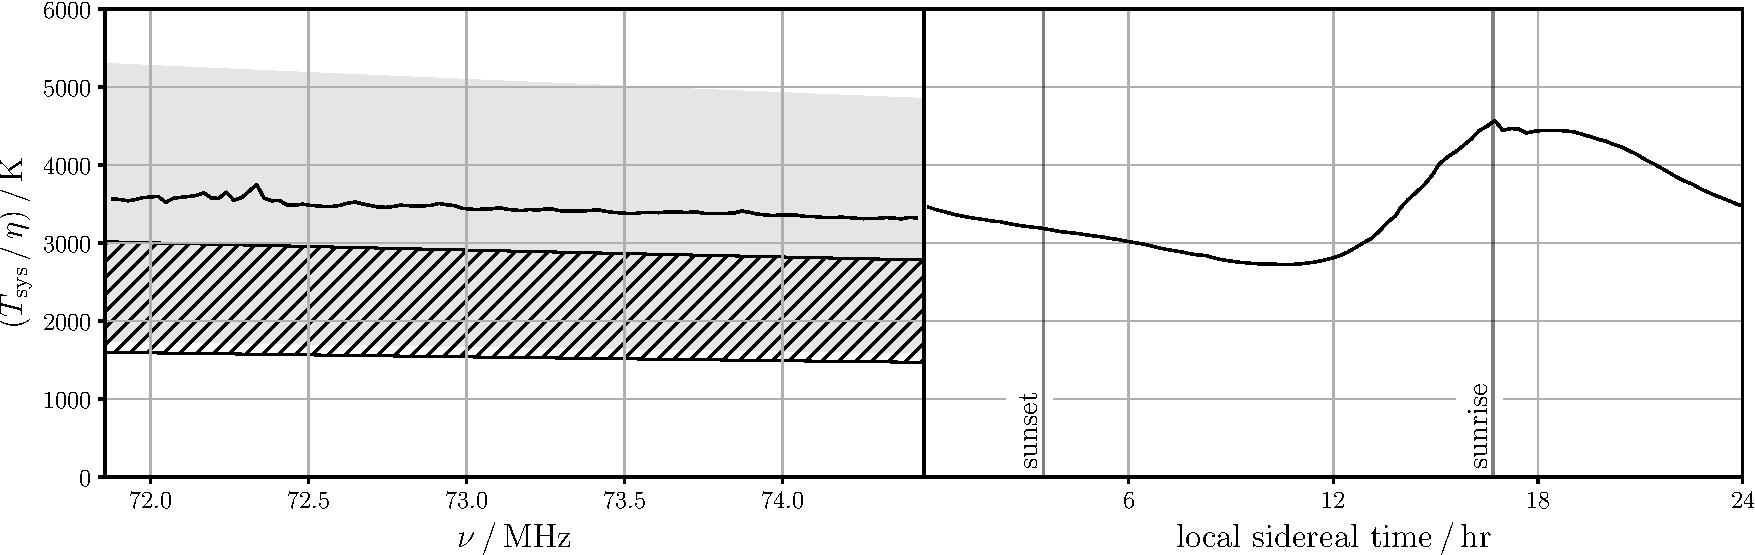
\includegraphics[width=\textwidth]{figures/chapter4/system-temperature}
    \caption{
        The system temperature $T_\text{sys}$ (scaled by the antenna efficiency $\eta$) measured as
        a function of frequency (left panel, solid black line), and local sidereal time (right
        panel, solid black line). The hatched region denotes the range of sky temperatures measured
        by the LEDA experiment \citep{2018MNRAS.478.4193P}. The shaded region denotes the range of
        sky temperatures measured by the EDGES experiment in the southern hemisphere
        \citep{2017MNRAS.464.4995M}.
    }
    \label{fig:Tsys}
\end{figure}

\begin{figure}
    \centering
    \includegraphics[width=\textwidth]{figures/chapter4/foreground-covariance-06}
    \caption{
        The angular power spectrum of the sky as measured by the OVRO-LWA at 73.260\,MHz.
        Measurements (with 95\% uncertainty) are indicated with red bars. The uncertainty is
        dominated by sample variance. The dashed black line is the best-fit power-law spectrum, and
        the solid black line is the best-fit solution when the power-law index is allowed to run.
        The dash-dot line is a model derived, in part, from the Haslam 408\,MHz sky map
        \citep{1981A&A...100..209H, 1982A&AS...47....1H, 2005ApJ...625..575S}.  The feature at
        $l\sim30$ is sensitive to the choice of covariance matrix, and is therefore likely
        instrumental.
    }
    \label{fig:foreground-covariance}
\end{figure}

The 21\,cm signal is expected to be unpolarized,\footnote{
    \citet{2017PhRvD..95h3010V} find that circular polarization may be used to measure primordial
    magnetic fields, but the amplitude of this effect is too small to consider measuring with
    existing low-frequency telescopes.
} so we form
Stokes-I visibilities from the mean of the $xx$ and $yy$ visibilities. Under this convention, the
covariance of the complex-valued Stokes-I visibilities is \citep[Chapter 9]{1999ASPC..180.....T}:
\begin{equation}
    \b C_\text{noise}
        = \left(
            \frac{2 k_B T_\text{sys}}{\eta A_\text{eff} \sqrt{2\Delta\nu\tau}}
        \right)^2 \b I\,,
\end{equation}
where $k_B$ is the Boltzmann constant, $T_\text{sys}$ is the system temperature, $\eta$ is the
antenna efficiency, $A_\text{eff}$ is the effective collecting area (each assumed to be the same for
all antennas), $\Delta\nu$ is the bandwidth, and $\tau$ is the total integration time.  The
effective collecting area of the antenna is related to the solid-angle of the primary beam $\Omega$
through $A_\text{eff} = \lambda^2 / \Omega$. At 73\,MHz, the OVRO-LWA dipoles have primary beams
with $\Omega \sim 2.4\,\text{sr}$ or $A_\text{eff}\sim 7\,\text{m}^2$.

OVRO-LWA dipoles are designed to be sky-noise dominated \citep[$\ge6$\,dB between 20--80\,MHz;
][]{2012PASP..124.1090H}. More precisely, the system temperature is given by
\begin{equation}
    T_\text{sys} \approx \eta T_\text{sky} + T_\text{pre-amp}\,,
\end{equation}
where $\eta$ is the antenna efficiency, $T_\text{sky}$ is the averaged brightness temperature of the
sky (primarily the galactic synchrotron emission) weighted by the primary beam pattern, and
$T_\text{pre-amp}$ is the noise temperature of the first amplifier in the analog signal path. We
expect $T_\text{pre-amp} \approx 250\,\text{K}$ and $\eta \lesssim 0.5$ \citep{2012PASP..124.1090H}.

The LEDA experiment hosted at the OVRO-LWA measured the brightness temperature of the diffuse
galactic emission in the northern hemisphere using the five radiometric antennas
\citep{2018MNRAS.478.4193P}. At 70~MHz, the brightness temperature varies between 1700\,K and
3200\,K with a relatively flat spectral index that varies between $-2.28$ and $-2.38$.  In the
southern hemisphere, the EDGES experiment measured that the brightness temperature of the sky at
150\,MHz varies between 257\,K and 842\,K with a spectral index that varies between $-2.50$ and
$-2.62$ \citep{2017MNRAS.464.4995M}. Extrapolating to 70\,MHz, we expect the beam-weighted sky
brightness temperature in the southern hemisphere to vary between 1700\,K and 6200\,K. The maximum
brightness temperature corresponds to sidereal time when the galactic center transits.

We measured the system temperature as a function of frequency and sidereal time using a five-point
stencil to suppress the contribution of the sky emission to the measured visibilities
\begin{align*}
    \Delta(\nu,\,t) = 4V(\nu, t)
                     &- V(\nu - 24\,\text{kHz},\,t)
                      - V(\nu,\,t - 13\,\text{s}) \\
                     &- V(\nu + 24\,\text{kHz},\,t)
                      - V(\nu,\,t + 13\,\text{s})\,,
\end{align*}
where $\Delta(\nu,\,t)$ is a quantity whose variance is 20 times larger than that of the measured
visibilities $V(\nu,\,t)$ at the given frequency $\nu$ and time $t$. Note that 24\,kHz is the native
frequency resolution of the OVRO-LWA and 13\,s is the integration time.  Therefore this stencil
takes the difference between each measured visibility and the bilinear interpolation from adjacent
frequency channels and time integrations. We then estimated the system temperature from the variance
of $\Delta$. The measured system temperature is shown in Figure~\ref{fig:Tsys} compared to the sky
temperature measured by LEDA and extrapolated from EDGES.  As expected, the system temperature
increases at lower frequencies due to the increasing sky brightness temperature, and varies
sidereally reaching a maximum as the galactic center transits the meridian. These measurements
suggest that the antenna efficiency $\eta \sim 0.25$. Although the system temperature varies with
time and frequency, we adopt a constant system temperature of $3500\eta\,\text{K}$ when computing
the sensitivity of the OVRO-LWA. We expect this approximation to potentially introduce errors of
$\sim 10\%$ to the computed sensitivity and error bars, which does not materially impact the results
presented in this paper.

\subsection{Foreground Covariance}\label{sec:foreground-covariance}

Under the assumption of a Gaussian random field, the covariance contributed by the sky can be
computed from the multi-frequency angular power spectrum:
\begin{equation}\label{eq:multi-frequency-angular-power-spectrum}
    \langle a_{lm}(\nu) \, a_{l^\prime m^\prime}^*(\nu^\prime)\rangle
        = C_l(\nu, \nu^\prime) \, \delta_{ll^\prime} \, \delta_{mm^\prime}\,,
\end{equation}
where the angled brackets denote an ensemble average over realizations of the sky, $a_{lm}(\nu)$ is
the spherical harmonic coefficient of the sky brightness at frequency $\nu$, $C_l(\nu, \nu^\prime)$
is the multi-frequency angular power spectrum at the multipole moment $l$, and between the
frequencies $\nu$ and $\nu^\prime$. The Kronecker delta is represented by $\delta$.  The
transfer-matrix $\b B$ describes how to relate the covariance of the spherical harmonic coefficients
to the covariance of the measurements themselves, such that
\begin{equation}\label{eq:maps-to-covariance}
    \b C_\text{sky} = \b B \b C^\prime_\text{sky} \b B^*\,,
\end{equation}
where $\b C_\text{sky}$ is a term in Equation~\ref{eq:sum-of-covariances}, and $\b
C^\prime_\text{sky}$ is a matrix whose elements are specified by
Equation~\ref{eq:multi-frequency-angular-power-spectrum}.

A common parameterization of $C_l(\nu_1, \nu_2)$ for foreground radio emission is
\citep{2005ApJ...625..575S}
\begin{eqnarray}\label{eq:cforeground}
    C_l^\text{fg}(\nu, \nu^\prime) =
    \sum_i &A_i& \left(\frac{l}{l_0}\right)^{-\alpha_i}
                 \left(\frac{\nu\nu^\prime}{\nu_0^2}\right)^{-\beta_i} \nonumber \\
           &\times&\exp\left(-\frac{(\log\nu-\log\nu^\prime)^2}{2\zeta_i^2}\right)\,,
\end{eqnarray}
where $A_i$ represents the overall amplitude of a foreground component.  $\alpha_i$ determines its
angular spectrum, and $\beta_i$ determines its frequency spectrum. Finally, $\zeta_i$ controls the
degree to which nearby frequency channels are correlated. The statement that foreground emission is
spectrally smooth here implies $\zeta_i \gg 1$ for each component. This parameterization allows for
multiple power-law foreground components and ensures that the covariance matrix is positive
definite.  Because the fractional bandwidth is small, in this paper we assume $\zeta_i^2 \gg
\log^2(\nu/\nu^\prime)$ such that
\begin{equation}
    C_l^\text{fg}(\nu, \nu^\prime) = \sqrt{C_l^\text{fg}(\nu)\,C_l^\text{fg}(\nu^\prime)}\,,
\end{equation}
where $C_l^\text{fg}(\nu) = C_l^\text{fg}(\nu, \nu)$ is the single-frequency angular power spectrum.

We measured the angular power spectrum of the foreground emission at each frequency channel using a
quadratic estimator \citep{1997PhRvD..55.5895T}. The angular power spectrum is given by
\begin{equation}
    C_l^\text{fg}(\nu) = \left[\b F^{-1} (\b q - \b b)\right]_l\,,
\end{equation}
where $\b F$ is the Fisher information matrix, $\b q$ is a quadratic function of the input data, and
$\b b$ is the bias due to thermal noise.  The elements of the Fisher matrix $\b F$ are given by
\begin{equation}
    F_{ll^\prime} = \sum_m \left\| \b b_{lm}^*\b C_m^{-1} \b b_{l^\prime m} \right\|^2\,,
\end{equation}
where $F_{ll^\prime}$ is the Fisher matrix element corresponding to the multipole numbers $l$ and
$l^\prime$, $\b b_{lm}$ is the column of the transfer matrix corresponding to $l$ and the azimuthal
quantum number $m$, and $\b C_m$ is the covariance matrix block corresponding to $m$. The elements
of $\b q$ and $\b b$ are given by
\begin{align}
    q_l &= \sum_m \left\| \b b_{lm}^*\b C_m^{-1} \b v_m \right\|^2 \\
    b_l &= \sum_m \left\| \b b_{lm}^*\b C_m^{-1} \b C^{1/2}_{\text{noise}, m} \right\|^2\,,
\end{align}
where $\b v_m$ is the vector of $m$-modes corresponding to the given value of $m$, and $\b
C_{\text{noise}, m}$ is the corresponding block of the noise covariance matrix.

The result of applying this quadratic estimator to the dataset at 73.260\,MHz (a representative
channel) can be seen in Figure~\ref{fig:foreground-covariance}. Broadly, the data can be described
with a power law in $l$, but the quality of the fit is somewhat poor. A single power-law fit gives
\begin{equation}
    C_l \sim 92. \times \left(\frac{l}{100}\right)^{-2.5} \,\text{K}^2\,.
\end{equation}
In fact, while this is a reasonable fit at $l > 75$, a shallower power-law index is preferred $l <
75$. If we allow for the power-law index to run, the best-fit model becomes:
\begin{equation}\label{eq:measured-cforeground}
    C_l \sim 85. \times \left(\frac{l}{100}\right)^{-3.2 + l/277.} \,\text{K}^2\,.
\end{equation}
A comparison of these two models can be seen in Figure~\ref{fig:foreground-covariance} in addition
to a model of the galactic synchrotron emission derived by \citet{2005ApJ...625..575S}, which
appears to underestimate the amplitude of $C_l$ by an order of magnitude.  Because the fractional
bandwidth of this measurement is small, essentially all reasonable spectral indices are permitted.
We adopt a fiducial spectral index of $-2.5$ as a compromise between the spectral indices measured
by LEDA and EDGES.

\subsection{Signal Covariance}\label{sec:signal-covariance}

\begin{figure}[t]
    \centering
    \includegraphics[width=\columnwidth]{figures/chapter4/flat-sky-approximation}
    \caption{
        The relative error involved with making the flat-sky approximation for a hat function power
        spectrum (i.e., the relative difference between Equations~\ref{eq:csignal-curved-sky} and
        \ref{eq:csignal-flat-sky}) with $l=10$ (solid line) and $l=100$ (dashed line). The hat
        function is centered at $k_\parallel=0.1\,\text{Mpc}^{-1}$ with a domain that extends from
        $0.095\,\text{Mpc}^{-1}$ to $0.105\,\text{Mpc}^{-1}$. The spikes in relative error
        correspond to when $C_l^\text{curved}(\Delta\nu) \approx 0$.
    }
    \label{fig:flat-sky-approximation}
\end{figure}

Given the isotropic three-dimensional spatial power spectrum of the 21\,cm brightness temperature
$P^{21}_z(k)$ with the wavenumber $k$ and at the redshift $z$, the multi-frequency angular
power spectrum $C_l(\nu, \nu^\prime)$ is given by
\begin{equation}\label{eq:csignal-curved-sky}
    C^{21}_l(\nu, \nu^\prime) =
        \frac{2}{\pi}
        \int
        P_z^{21}(k) \,
        j_l(k r_z) \,
        j_l(k r_{z^\prime}) \,
        k^2 \, \d k\,,
\end{equation}
where $r_z$ is the comoving distance to the redshift $z$ (specified by the frequency $\nu$), and
$j_l(x)$ is the spherical Bessel function of the first kind. In the flat-sky approximation,
Equation~\ref{eq:csignal-curved-sky} can be simplified to
\begin{equation}\label{eq:csignal-flat-sky}
    C^{21}_l(\nu, \nu^\prime) \approx
        \frac{1}{\pi r_z r_{z^\prime}}
        \int
        P_z^{21}(k_\perp, k_\parallel) \,
        \cos\left(k_\parallel \Delta r_z\right)
        \, \d k_\parallel\,,
\end{equation}
where $k_\perp = l/r_z$ and $k_\parallel = \sqrt{k^2-k_\perp^2}$.  See
Appendix~\ref{app:spatial-to-angular} for a derivation of this approximation and the assumptions
that must be satisfied for it to be a reasonable approximation.

If $P_z^{21}(k_\perp, k_\parallel)$ is additionally assumed to be a piece-wise linear function,
Equation~\ref{eq:csignal-flat-sky} can be evaluated analytically. Under this assumption,
$P_z^{21}(k_\perp, k_\parallel)$ can be represented using linear hat functions (triangular functions
in two dimensions), such that
\begin{align}
    P_z^{21}(k_\perp, k_\parallel) &= \sum_\alpha p_\alpha
        \times {\rm hat}_\alpha(k_\perp, k_\parallel)
        \label{eq:palpha} \\
    C^{21}_l(\nu, \nu^\prime) &\approx
        \frac{1}{\pi r_z r_{z^\prime}}
        \sum_\alpha p_\alpha H_\alpha(\Delta r_z)
\end{align}
where $H_\alpha(\Delta r_z) = \int {\rm hat}_\alpha(k_\perp, k_\parallel) \, \cos\left(k_\parallel
\Delta r_z\right) \, \d k_\parallel$.

The flat-sky approximation is valid only when the power spectrum is smooth enough for rapid
oscillations in the spherical Bessel functions to cancel out. The hat functions are
non-differentiable, and so we must compute the error associated with this pixelization of the power
spectrum. Figure~\ref{fig:flat-sky-approximation} gives the relative error on the computed angular
power spectrum for a fiducial hat function power spectrum. Generally the error is $10^{-4}$, but can
reach to $10^{-1}$ at values where $C_l \approx 0$. This is an acceptable error in the context of
this paper, but future experiments may wish to experiment with differentiable basis functions.

When selecting a fiducial model for the 21\,cm power spectrum we prefer to remain unopinionated, and
therefore adopt a flat power spectrum with a single free parameter, the overall amplitude of the
dimensionless power spectrum $\Delta_{21}$:
\begin{equation}
    P_\text{fiducial}^{21}(k) = \frac{2\pi^2}{k^3}\Delta_{21}^2\,.
\end{equation}
Prior to the recent detection of an absorption feature centered at 78\,MHz by
\citet{2018Natur.555...67B}, the amplitude of the power spectrum was generally predicted to be
$\Delta_{21} < 20\,\text{mK}$ at $z\sim 20$ \citep[e.g.,][]{2014MNRAS.437L..36F}. However, more
recent predictions in the context of the measured 78\,MHz absorption feature predict a much brighter
power spectrum \citep[e.g.][]{2018Natur.555...71B, 2018arXiv180503254K}. We therefore adopt
$\Delta_{21} = 140\,\text{mK}$ as a fiducial power spectrum amplitude, which assumes that
interactions between baryons and dark matter are important for cooling the IGM in the early
universe. The amplitude of the fiducial 21\,cm signal is primarily used to determine which modes
should be kept by the foreground filter described in the following section. Therefore, if the reader
is skeptical of this selection of the fiducial 21\,cm signal, they may simply choose to interpret
the results as if the foreground filter was weaker than expected.

\section{Foreground Filtering}\label{sec:foreground-filtering}

\begin{figure}
    \centering
    \includegraphics[width=\textwidth]{figures/chapter4/foreground-filtering-illustration}
    \caption{
        Illustration of the action of foreground filtering on each of the covariance matrices
        discussed in \S\ref{sec:sensitivity}. The left column corresponds to the noise covariance
        matrix, the middle column corresponds to the high-redshift 21\,cm contribution to the
        covariance, and the right column corresponds to the foreground covariance matrix. The top
        row is before any filtering has been applied, the middle row is after the first KL
        transform, and the bottom row is after the second KL transform.
    }
    \label{fig:foreground-filtering-illustration}
\end{figure}

\begin{figure}[t]
    \centering
    \includegraphics[width=\columnwidth]{figures/chapter4/cylindrical-power-spectrum-error-bars}
    \caption{
        The fractional increase in the size of the error bars in each power spectrum bin due to the
        application of a double KL transform foreground filter (moderate strength).
    }
    \label{fig:error-bars-increase}
\end{figure}

\begin{figure}[t]
    \centering
    \includegraphics[width=\columnwidth]{figures/chapter4/foreground-filtering-schematic}
    \caption{
        Mollweide projected illustration of the sky where shaded regions are down-weighted by the
        foreground filter. From darkest to lightest, these regions of the sky are filtered by the
        mild, moderate, and extreme foreground filters respectively.
    }
    \label{fig:foreground-filtering-schematic}
\end{figure}

In the preceding sections, we have derived and---where appropriate---measured the contribution of
thermal noise, foreground emission and the cosmological 21\,cm emission to the complete covariance
matrix of the data. This was possible because the transfer matrix $\b B$ is block-diagonal with
respect to $m$, and we assumed that the sky emission is a Gaussian-random field (i.e., there are no
correlations between different values of $m$). Without these properties the full covariance matrix
is generally too large to represent and manipulate on any existing computer.
\citet{2014ApJ...781...57S, 2015PhRvD..91h3514S} were therefore able to derive a new foreground
filtering technique that exploits knowledge of the full covariance matrix. This filter is called the
double Karhunen--Lo\`{e}ve transform (double KL transform). In this section we will briefly
summarize the action of this foreground filter and demonstrate its application to the OVRO-LWA. We
will finally attempt to develop an intuitive understanding by relating its behavior to the
``foreground wedge'' commonly seen in the literature
\citep[e.g.,][]{2012ApJ...745..176V,2012ApJ...756..165P,2015ApJ...804...14T}.

The KL transform is closely related to the generalized eigenvalue problem. For two Hermitian,
positive definite matrices $\b C_1, \b C_2 \in \mathbb{C}^N$, we would like to find all pairs of
eigenvalues
$\lambda_i$ and eigenvectors $\b v_i$ for which
\begin{equation}
    \b C_1 \b v_i = \lambda_i \b C_2 \b v_i\,.
\end{equation}
Because both matrices are Hermitian, it quickly follows that the eigenvalues $\lambda_i$ must be
real. Because both matrices are additionally positive definite, it follows that the eigenvalues
$\lambda_i$ must all be positive. Furthermore we can select the normalization of the eigenvectors
such that
\begin{align}
    \b v_i^* \b C_1 \b v_i &= \lambda_i \\
    \b v_i^* \b C_2 \b v_i &= 1\,.
\end{align}
Under this convention the eigenvalues have a simple interpretation as the ratio of the mode-power
contained in $\b C_1$ relative to $\b C_2$. All $N$ eigenvalues and eigenvectors can be conveniently
found with a single call to LAPACK \citep{Anderson:1990:LPL:110382.110385}.

In \S\ref{sec:foreground-covariance} we derived and measured a model for the foreground contribution
to the data covariance $\b C_\text{fg}$. In \S\ref{sec:signal-covariance} we projected a fiducial
model 21\,cm power spectrum to a multi-frequency angular power spectrum, and therefore derived its
contribution to the data covariance $\b C_\text{21}$. We can solve the generalized eigenvalue
problem for the eigenvectors (arranged as columns within the matrix $\b L$) that simultaneously
diagonalize both matrices (called the KL transform):
\begin{align}
    \b L\b C_\text{fg}\b L^* &= \b\Lambda \\
    \b L\b C_\text{21}\b L^* &= \b I \,,
\end{align}
where $\b\Lambda$ is a diagonal matrix, and $\b I$ is the identity matrix. The foreground filter is
simply constructed by selecting only the eigenvectors for which the corresponding eigenvalue (i.e.,
the foreground--signal power ratio) is less than some value $\epsilon_\text{filter}$ selected by the
observer. The application of this filter to a fiducial set of models can be seen in the second row
of Figure~\ref{fig:foreground-filtering-illustration}. The signal covariance matrix has been
diagonalized and the power in each remaining mode is greater than the surviving power in the
foreground covariance matrix. The off-diagonal elements in the foreground covariance matrix are due
to numerical errors. The possible effect of these numerical errors on the efficacy of the foreground
filter is noted here, but is out of the scope of the current work.

Much emphasis has been placed on maintaining the integrity of the ``foreground wedge'' in the next
generation of 21\,cm telescopes. In its simplest form, the existence of the foreground wedge is a
statement that most foreground radio emission that observers have to contend with when trying to
detect the cosmological 21\,cm is spectrally smooth. A simple Fourier transform of an image cube
therefore leads to most contamination occupying the space where $k_\parallel$ (the line of sight
wavenumber) is small. However, due to the chromatic nature of interferometers (specifically that the
fringe spacing $\propto b/\lambda$ where $b$ is the baseline length and $\lambda$ is the
wavelength), this contamination is spread out into a wedge-like structure. Additional chromaticity
in, for example, the bandpass or antenna primary beam leads to the contamination even leaking out of
the wedge. In the event of too much leakage, the observer has lost their ability to measure the
cosmological 21\,cm transition.

In contrast, the KL transform automatically finds the optimal linear combination of the dataset for
separating foregrounds using all available information built into the models. This includes
information on the frequency spectrum of the foregrounds as well as their angular structure, which
can lead to scenarios where the KL transform can filter foreground emission that cannot be avoided
with a delay filter. There is, of course, a caveat that the KL transform requires sufficiently
detailed models for the instrument and foreground emission. However, it is not necessarily optimal
to remain completely apathetic to the structure of foreground emission, and most collaborations are
expending significant effort to characterize their instruments.

A single KL transform, however, leads to large off-diagonal elements in the noise covariance matrix
(see the second row of Figure~\ref{fig:foreground-filtering-illustration}). Therefore
\citet{2014ApJ...781...57S,2015PhRvD..91h3514S} introduced a second KL transform that diagonalizes
the noise covariance matrix. This second matrix composed of eigenvectors will be denoted with $\b
W$. In total we therefore have
\begin{equation}
    \b C_\text{filtered}
        = \underbrace{\b W^*\b L^*\b C_\text{21}\b L\b W}_{\b S}
        + \underbrace{\b W^*\b L^*(\b C_\text{fg} + \b C_\text{noise})\b L\b W}_{\b I}\,,
\end{equation}
where $\b C_\text{filtered}$ is the data covariance matrix after applying the double KL transform
foreground filter, $\b S$ is a real diagonal matrix, and $\b I$ is the identity matrix. The diagonal
elements of $\b S$ give the expected signal--noise ratio in each mode.  The foreground filter is
applied to the measured $m$-modes by simply computing
\begin{equation}
    \b v_\text{filtered} = \b W^*\b L^*\b v\,.
\end{equation}

In this paper we will repeat the analysis using three different values for the foreground filtering
signal--foreground threshold $\epsilon_\text{filter}$. This will allow us to assess the performance
of the foreground filter and degree to which residual foreground contamination may be affecting the
measurement. We will adopt the terminology ``strong,'' ``moderate,'' and ``mild'' to mean:
\begin{align*}
    \epsilon_\text{filter} &= 0.1 & \text{(``strong'' foreground filtering)} \\
    \epsilon_\text{filter} &= 1   & \text{(``moderate'' foreground filtering)} \\
    \epsilon_\text{filter} &= 10  & \text{(``mild'' foreground filtering)}\,.
\end{align*}
Now we will build a physical intuition for understanding the operation of the double KL transform
foreground filter.

Figure~\ref{fig:error-bars-increase} illustrates the fractional increase in error bars associated
with applying the moderate foreground filter. In the space of a cylindrically binned power spectrum,
the action of the filter is to discard linear combinations of the dataset with low $k_\parallel$ and
low $k_\perp$. This manifests itself as a decrease in sensitivity---equivalently an increase in the
error bars---in this region of parameter space.  High $k_\parallel$ modes are computed from rapid
frequency differences, whereas low $k_\parallel$ modes are slowly varying in frequency. Because the
foreground emission is spectrally smooth, it tends to corrupt modes with low $k_\parallel$. The
pattern of this contamination is known as the foreground wedge. However, the foreground filter
additionally removes emission on large angular scales (low $k_\perp$). This arises because the
foreground filter is aware that the foreground emission is brighter on larger angular scales (see
Figure~\ref{fig:foreground-covariance} and Equation~\ref{eq:measured-cforeground}).

As illustrated in Figure~\ref{fig:foreground-filtering-schematic}, the foreground filter also tends
to remove emission in two separate parts of the sky: low declinations that are never seen at high
elevations from the OVRO-LWA, and high declinations around the North Celestial Pole (NCP).  This
filtering of high and low declinations can be seen in
Figure~\ref{fig:spherical-power-spectra-filter-strength}, which is a Tikhonov-regularized image of
the sky constructed from the post-filtered data.

The OVRO-LWA is a zenith pointing drift-scanning instrument.  Therefore foreground emission located
far from zenith has a large path difference between antennas. This large path difference leads to
additional frequency structure that allows the foreground emission to contaminate higher values of
$k_\parallel$ \citep{2012ApJ...752..137M}.  Similarly, \citet{2015ApJ...804...14T} derived the
impact of widefield effects on the foreground contamination and found that baseline foreshortening
can lead to additional galactic synchrotron emission on large angular scales contaminating the
measurement. This foreground emission from low-elevations is problematic. The double KL transform
suppresses the contribution of these low elevations to the measurement.

Emission from the vicinity of the NCP is characterized by its low fringe-rate. As the Earth rotates,
emission located here moves slowly through the fringes of the interferometer. Therefore this
emission is predominantly characterized by low values of $m$. The foreground emission, however, is
brightest relative to the cosmological 21\,cm emission at low values of $l$ (large angular scales).
Because $m \le l$ for a given value of $l$, low values of $m$ are disproportionately contaminated by
the brightest diffuse components of the foreground emission. In fact, for the fiducial foreground
and signal models presented in \S\ref{sec:foreground-covariance} and \S\ref{sec:signal-covariance}
respectively, the the foreground--signal ratio of the most favorable mode is $\propto m^{-3.5}$.
This is a reflection of the fact that emission with a higher fringe rate tends to be smaller in
angular extent.  Consequently, the foreground filter aggressively discards information from small
values of $m$ and the emission located at the NCP is collateral damage because it can be difficult
to separate from the diffuse foreground emission. This can be seen in
Figure~\ref{fig:foreground-filtering-schematic} where increasing the strength of the foreground
filter increases the area around the NCP that is down-weighted.

%%%%%%%%%%%%%%%%%%%%%%%%%%%%%%%%%%%%%%%%%%%%%%%%%%%%%%%%%%%%%%%%%%%%%%%%%%%%%%%%%%%%%%%%%%%%%%%%%%%%
\section{Results and Error Analysis}\label{sec:results}

\begin{sidewaysfigure}[p]
    \centering
    \begin{tabular}{c}
        \includegraphics[width=0.75\textwidth]{figures/chapter4/filtered-sky-map-colorbar}\\
        \includegraphics[width=0.75\textwidth]{figures/chapter4/spherical-power-spectrum-filter-strength}\\
    \end{tabular}
    \caption{
        (top) Mollweide projected image of the sky after point source removal and moderate
        foreground filtering. The dominant residual feature in the residuals is associated with the
        Sun.
        (bottom) The power spectrum estimated without point source removal (left) and with point
        source removal (right) at a range of filter strengths. Points correspond to the estimated
        power spectrum amplitude and the dashed lines correspond to the computed thermal noise.
        Mild foreground filtering is red, moderate foreground filtering is black, and extreme
        foreground filtering is blue.
    }
    \label{fig:spherical-power-spectra-filter-strength}
\end{sidewaysfigure}

We will use a quadratic estimator to measure the spatial power spectrum of 21\,cm fluctuations
\citep{1997PhRvD..55.5895T}. In particular we estimate the coefficients $p_\alpha$, which are
defined in Equation~\ref{eq:palpha}. As described by \citet{2003NewA....8..581P}, the observer may
tune the estimator by selecting a windowing function that produces desired properties. For example,
given the measured data $\b v$, the full covariance matrix $\b C$, and the Fisher information matrix
$\b F$, the unwindowed and minimum variance estimates of the power spectrum amplitude are
\begin{align}
    \hat{p}_\alpha^\text{unwindowed} &= \sum_\beta [\b F^{-1}]_{\alpha\beta}\,(q_\beta-b_\beta) \\
    \hat{p}_\alpha^\text{min. variance} &= \left(\sum_\beta
        F_{\alpha\beta}\right)^{-1}(q_\beta-b_\beta)\,,
\end{align}
where
\begin{align}
    q_\alpha &= \b v^*\b C^{-1}\frac{\partial\b C}{\partial p_\alpha}\b C^{-1}\b v \\
    b_\alpha &= \tr\left(\b C^{-1}\frac{\partial\b C}{\partial p_\alpha}
                         \b C^{-1}\b C_\text{noise}\right) \\
    F_{\alpha\beta} &= \tr\left(\b C^{-1}\frac{\partial\b C}{\partial p_\alpha}
                                \b C^{-1}\frac{\partial\b C}{\partial p_\beta}\right)\,.
\end{align}
Directly computing $F_{\alpha\beta}$ from its definition is computationally expensive, and so we
compute an approximation of the Fisher information matrix using the iterative Monte Carlo scheme
described by \citet{2013PhRvD..87d3005D}.

We will make exclusive use of the minimum variance estimator in this paper because it is relatively
insensitive to errors in the Fisher information matrix, which are inevitable due to the Monte Carlo
computation. Additionally, the unwindowed estimator can compound numerical errors when the condition
number of $\b F$ is large.\footnote{
    The condition number of a matrix $\b A$ is $\kappa(\b A) = \|\b A\|\,\|\b A^{-1}\|$ and
    describes the error introduced when solving the linear equation $\b A\b x=\b b$ for the vector
    $\b x$. As a general rule of thumb, if $\log_{10}\kappa(\b A) = N$, one can expect to lose $N$
    digits of precision after computing $\b A^{-1}\b b$.
}

In Figure~\ref{fig:spherical-power-spectra-filter-strength} we present the results of the quadratic
estimator with and without point source removal, and across the range of foreground filter
strengths. These estimates are, across the board, severely limited by systematic errors. This is
readily apparent due to the extreme amplitude of the estimated power.  We therefore interpret these
measurements as upper limits $\Delta_{21}^2 \lesssim (10^4\,\text{mK})^2$ at $k\approx
0.10\,\text{Mpc}^{-1}$.

As the strength of the foreground filter is increased more information is lost by the filter. This
is seen in the window functions of the quadratic estimator. With mild foreground filtering, the
window functions are roughly evenly spaced between $k=0.10\,\text{Mpc}^{-1}$ and
$0.35\,\text{Mpc}^{-1}$. With extreme foreground filtering, all of the measurements are instead
concentrated around $k=0.15\,\text{Mpc}^{-1}$, which reflects the loss of information at other
values of the wavenumber $k$.

After initial calibration and stationary component removal, we attempted to subtract the eight
brightest point sources in the northern hemisphere in addition to the Sun. The brightest of these
sources were removed with direction-dependent calibrations. The fainter sources were simply
subtracted after fitting for their flux and position (attempting to account for ionospheric
scintillation and refraction). The Sun was removed using a resolved source model. With mild
foreground filtering, this point source removal leads to a $\sim2\times$ reduction in the power
spectrum amplitude.

However, the efficacy of the foreground filter materially differs between the datasets where bright
point sources have and have not been removed. Without point source removal, increasing the strength
of the foreground filter leads to a reduction of the estimated power. This reflects the fact that
the foreground filter is removing increasing amounts of foreground contamination. In contrast, if
point sources have been subtracted, the power spectrum amplitude is insensitive to the strength of
the foreground filter. While the point source removal routine leads to less foreground contamination
in the absence of foreground filtering, it also restricts the effectiveness of the foreground
filter. This suggests that the point source removal routine introduces additional errors into the
dataset that inhibit the action of the foreground filter.

We will now attempt to diagnose the source of these residual systematic errors that limit this
measurement. While doing this, we will adopt the moderate foreground filter as the fiducial
foreground filter due to its action as a compromise between the amount of foreground emission
removed and resolution in the wavenumber $k$.

\subsection{Even--Odd Jackknife}

\begin{sidewaysfigure}[p]
    \centering
    \begin{tabular}{c}
        \includegraphics[width=0.75\textwidth]{figures/chapter4/even-odd-sky-map-colorbar}\\
        \includegraphics[width=0.75\textwidth]{figures/chapter4/spherical-power-spectrum-even-odd}\\
    \end{tabular}
    \caption{
        (top) Mollweide projection of the sky in galactic coordinates after differencing even and
        odd-numbered integrations. The Sun is the dominant artifact in this image due to the
        sporadic failure of source subtraction. Large residuals are also present at low declinations
        that do not rise above $10\arcdeg$ elevation. These low-elevation artifacts are generated by
        RFI.
        (bottom) The power spectrum estimated without point source removal (left) and with point
        source removal (right). Point correspond to the estimated power spectrum amplitude and the
        dashed line corresponds to the computed thermal noise. Red and blue points are estimates
        from the even and odd numbered integrations respectively. Black points are estimates after
        computing the difference between the two halves of data.
    }
    \label{fig:spherical-power-spectra-even-odd}
\end{sidewaysfigure}

Errors arising from variations on rapid timescales---the timescale of a single correlator dump---can
be revealed through the comparison of results obtained data using only even-numbered integrations
and the interleaving odd-numbered integrations. These two halves of the dataset have independent
thermal noise with additional errors due to ionospheric scintillation, RFI and source subtraction
errors.

In prior work we observed that ionospheric scintillation generates $\sim10\%$ fluctuations in the
flux of a point source on 13\,s timescales at 73\,MHz \citep{2018AJ....156...32E}. The position of a
source varies more slowly by up to $4\arcmin$ on 10\,min timescales. Therefore comparing even and
odd-numbered integrations will reveal errors arising from ionospheric scintillation, but not
necessarily from variable ionospheric refraction.

Figure~\ref{fig:spherical-power-spectra-even-odd} contains a map of the sky constructed from
differencing the even and odd datasets (after point source removal).  This map is almost
featureless. If ionospheric scintillation was contributing a substantial amount of additional noise
to the measurement, we would expect to see enhanced residuals in the vicinity of bright point
sources. Instead, the dominant features are a $\sim50\,\text{K}$ residual at the location of the
Sun, and some artifacts that manifest at low declinations that do not rise above $10\arcdeg$
elevation (likely generated by RFI). We therefore conclude that over a long 28\,hr integration, the
ionospheric scintillation has averaged down and is not the dominant source of error.

The bottom panel of Figure~\ref{fig:spherical-power-spectra-even-odd} compares the amplitude of the
estimated power spectrum after differencing the even and odd-numbered integrations. Differencing the
two halves of the dataset cancels out the majority of the residual contamination of foreground
emission into the measurement. Therefore the power spectrum decreases in amplitude. The improvement
is roughly one order of magnitude before source subtraction and only a factor of 2--3 after source
subtraction. Point source removal is conducted independently on each integration, sporadic errors
and source subtraction residuals will therefore also tend to manifest on the timescale of a single
integration. This measurement therefore suggests that source subtraction residuals could be a
limiting factor for this estimate of the 21\,cm power spectrum.

\subsection{Day--Night Jackknife}

\begin{sidewaysfigure}[p]
    \centering
    \begin{tabular}{c}
        \includegraphics[width=0.75\textwidth]{figures/chapter4/day-night}\\
        \includegraphics[width=0.75\textwidth]{figures/chapter4/spherical-power-spectrum-day-night}\\
    \end{tabular}
    \caption{
        (top) Orthographic projection of the sky constructed from data collected only during the day
        (left), and only during the night (right).
        (bottom) The power spectrum estimated without point source removal (left) and with point
        source removal (right). Points correspond to the estimated power spectrum amplitude and the
        dashed line corresponds to the computed thermal noise. Measurements from the day are red,
        and measurements from the night are blue.
    }
    \label{fig:spherical-power-spectra-day-night}
\end{sidewaysfigure}

The dominant subtraction residual in the preceding section is associated with the Sun, which is a
difficult source to cleanly subtract due to its complex structure. We can therefore split the data
into two halves: data collected while the Sun is above the horizon, and below the horizon. The data
collected during the night has a number of advantages. Specifically, subtraction residuals
associated with the Sun cannot impact data collected during the night.  Additionally the ionospheric
Total Electron Content (TEC) is lower during the night because the Sun acts as a source of
ionization for the ionosphere. Specifically, the median vertical TEC measured within 200\,km of OVRO
rose to 20\,TECU during the day, but drops to 6\,TECU during the night. There were no geomagnetic
storms during the observing period and the fact that these observations were collected during the
winter months generally contributes to a reduction in the ionospheric TEC.  Finally, due to the time
of year, the sky temperature is lower at night. For these reasons, we generally expect an
improvement in the nighttime data with respect to the daytime data.

In principle, $m$-mode analysis requires that data be collected for a full sidereal day because the
$m$-modes are computed from the Fourier transform of the visibilities with respect to sidereal time.
We relax that requirement here.  When selecting half the data, we additionally apply a
Blackman--Harris window function to prevent ringing. Tikhonov-regularized images made from just the
daytime and nighttime data can be seen in Figure~\ref{fig:spherical-power-spectra-day-night}. These
dirty images serve as a proof of concept that $m$-mode analysis can reasonably be applied to
datasets without a full sidereal day's worth of data.

We estimated the power spectrum from each half of data and the results are presented in
Figure~\ref{fig:spherical-power-spectra-day-night}. Restricting the observations to nighttime-only
leads to a substantial improvement in the power spectrum limits both with and without point source
removal. In fact the measurements with and without point source removal are now comparable. This
suggests the point source subtraction residuals are less of an issue in the nighttime data due to
the fact that (due to the time of year) there are fewer bright point sources that were removed.

\subsection{$xx$--$yy$ Jackknife}

\begin{sidewaysfigure}[p]
    \centering
    \begin{tabular}{c}
        \includegraphics[width=0.75\textwidth]{figures/chapter4/xx-yy-sky-map-colorbar}\\
        \includegraphics[width=0.75\textwidth]{figures/chapter4/spherical-power-spectrum-xx-yy}\\
    \end{tabular}
    \caption{
        (top) Mollweide projection of the sky in galactic coordinates after differencing the $xx$
        and $yy$ correlations. Note that this is not true linear polarization because it does not
        account for the full polarization of the antenna response pattern.
        (bottom) The power spectrum estimated without point source removal (left) and with point
        source removal (right). Point correspond to the estimated power spectrum amplitude and the
        dashed line corresponds to the computed thermal noise. Red and blue points are estimates
        from the $xx$ and $yy$ correlations respectively. Black points are estimates from the mean
        of the $xx$ and $yy$ correlations.
    }
    \label{fig:spherical-power-spectrum-xx-yy}
\end{sidewaysfigure}

The polarization angle of linearly polarized emission rotates as it propagates through a magnetized
plasma \citep[e.g.,][]{2014A&A...568A.101J}. The rotation angle is $\propto\lambda^2$, where
$\lambda$ is the wavelength of the radiation. Therefore instrumental polarization leakage from a
linear polarization (Stokes~$Q$ or Stokes~$U$) into total intensity (Stokes~$I$) can introduce
additional spectral structure into the foreground emission that is not accounted for in our
currently unpolarized analysis.

If Faraday-rotated linearly polarized emission is a problem, it will be exacerbated by computing the
power spectrum from the $xx$ correlations and $yy$ correlations separately. For this comparison, the
transfer matrix $\b B$ must be recomputed using the correct response pattern for the individual
dipoles. An image of the sky computed from the difference of the $xx$ and $yy$ correlations is shown
in Figure~\ref{fig:spherical-power-spectrum-xx-yy}. This map is related to the linear polarization
of the sky, but does not account for the full polarization of the beam, and therefore includes some
amount of instrumental polarization.

We estimated the 21\,cm power spectrum from the $xx$ and $yy$ correlations. This estimate is shown
in Figure~\ref{fig:spherical-power-spectrum-xx-yy}. The estimates are comparable to the total
intensity estimate and we therefore conclude that polarization leakage is not currently a major
source of systematic error.

\subsection{Calibration Errors}\label{sec:calibration-errors}

\begin{sidewaysfigure}[p]
    \centering
    \begin{tabular}{c}
        \includegraphics[width=0.75\textwidth]{figures/chapter4/channel-difference-sky-map-colorbar}\\
        \includegraphics[width=0.75\textwidth]{figures/chapter4/spherical-power-spectrum-gain-errors}\\
    \end{tabular}
    \caption{
        (top) Mollweide projection of the sky in galactic coordinates after differencing two
        adjacent 240\,kHz frequency channels.
        (bottom) Simulated power spectrum estimates as a result of a foreground model and gain
        errors that are incoherent between antennas (left) and coherent between antennas (right).
        Blue corresponds to 0.1\% errors, black corresponds to 1\% errors, and red corresponds to
        10\% errors in the complex gains.
    }
    \label{fig:spherical-power-spectrum-gain-errors}
\end{sidewaysfigure}

Multiple authors have investigated the impact of calibration errors on an experiment's ability to
separate foreground emission from the cosmological 21\,cm signal \citep{2016MNRAS.461.3135B,
2017MNRAS.470.1849E}. In this section we will compute the impact of calibration errors on the double
KL transform foreground filter.

In this calculation will simulate a realistic set of visibilities for the foreground emission, and
introduce errors into the calibration before applying the double KL transform filter. Finally we
will estimate the power spectrum amplitude as a way to characterize the amount of contamination
associated with the calibration errors.

The angular structure of the foreground model used here is measured from the data itself (shown in
the bottom panel of Figure~\ref{fig:before-after-source-removal-sky-maps}), but the frequency
dependence of this emission is chosen to be a power-law with a fiducial spectral index of $-2.3$.
This spectral index was chosen to be consistent with the results reported by LEDA
\citep{2018MNRAS.478.4193P}, but due to the small fractional bandwidth of this measurement, we
expect these results to be insensitive to the specific choice of spectral index. The set of
$m$-modes we expect to measure with the interferometer $\b v_\text{simulated}$ is computed:
\begin{equation}
    \b v_\text{simulated} = \b B\b a_\text{simulated}\,,
\end{equation}
where $\b B$ is the transfer matrix, and $\b a_\text{simulated}$ is a vector of the spherical
harmonic coefficients of the foreground model.

At this point the simulated $m$-modes are corrupted with calibration errors. We explore two
possibilities:
\begin{enumerate}
    \item each antenna and frequency channel receives an incorrect gain calibration
    \item each frequency channel receives an incorrect gain calibration, but this error is coherent
        across antennas
\end{enumerate}
In each case, the gain errors are drawn from a complex normal distribution, and the amplitude of the
error is varied between 0.1\%, 1\%, and 10\%. The former case is coined ``random gain errors'' to
indicate that each antenna is given an error in its complex gain calibration. The latter case is
coined ``random bandpass errors'' to indicate that the overall bandpass of the interferometer is
perturbed. The impact of these calibration errors can be seen in
Figure~\ref{fig:spherical-power-spectrum-gain-errors}.

In order to avoid biasing the 21\,cm power spectrum, these results indicate that the gain
calibration must be derived to an accuracy better than 0.1\%.  A general rule of thumb for the
OVRO-LWA is that for equal amplitude errors, the foreground contamination generated by bandpass
errors that are coherent across all antennas are an order of magnitude worse than for the random
gain errors (in units of $\Delta_{21}^2$). Therefore to achieve a comparable level of foreground
contamination, the overall bandpass of the interferometer must be known to better than 0.01\%.

The dataset presented in this paper is systematically limited at roughly $\Delta_{21}^2 \sim
(10^4\,\text{mK})^2$. These limits are therefore consistent with $\sim 1\%$ errors in the overall
bandpass of the interferometer. The top panel of
Figure~\ref{fig:spherical-power-spectrum-gain-errors} therefore presents the fractional difference
in the sky images between two adjacent frequency channels (after averaging down to 240\,kHz channel
resolution). The residuals in this sky map are typically 2\%--3\%, but generally do not correlate
with the sky brightness. We therefore conclude that between adjacent 240\,kHz channels, the bandpass
error is less than 1\%.

In fact, the structure of the residuals in Figure~\ref{fig:spherical-power-spectrum-gain-errors}
suggests a different terrestrial source. Terrestrial sources of radio emission do not move through
the sky at a sidereal rate. Therefore when constructing images of the sky, this contaminating
emission tends to be smeared along rings of constant declination. These ring-like structures are
clearly visible in Figure~\ref{fig:spherical-power-spectrum-gain-errors} alongside some larger scale
diffuse structures.

However, if we attribute the residual emission entirely to gain errors, then these simulations
suggest that the antenna gains are known only to within a couple percent, which when considered
alongside the RFI that contaminates the measurement, is likely sufficient to explain the current
systematic limitations of our dataset.

%%%%%%%%%%%%%%%%%%%%%%%%%%%%%%%%%%%%%%%%%%%%%%%%%%%%%%%%%%%%%%%%%%%%%%%%%%%%%%%%%%%%%%%%%%%%%%%%%%%%
\section{Conclusion}\label{sec:conclusion}

In this paper we estimated the amplitude of the 21\,cm power spectrum of the Cosmic Dawn with 28\,hr
of data from the OVRO-LWA. This measurement was severely limited by systematic errors and therefore
we interpret our measurements as upper limits, which are currently the most sensitive at this epoch
and the first measurement at $z > 18$. We measured $\Delta_{21}^2 \lesssim (10^4\,\text{mK})^2$ at
$k \approx 0.10\,\text{Mpc}^{-1}$.

In making this measurement, we demonstrated the first application of the double KL transform
foreground filter to a measured dataset. We demonstrated that the application of this foreground
filter can lead to improved power spectrum limits, and in combination with Tikhonov-regularized
imaging, we developed a physical intuition for the action of the foreground filter.  The double KL
transform derives its action from models for the foreground and 21\,cm signal covariance. We
measured the angular power spectrum of the foreground emission and found that the power-law index
appears to steepen on large angular scales ($l < 50$). The 21\,cm signal covariance is derived from
the flat-sky approximation, which we derive in Appendix~\ref{app:spatial-to-angular}.

Although application of the foreground filter leads to some improvement in our measurement of the
21\,cm power spectrum, the improvement was relatively modest. This is essentially a reflection of
the fact that the true covariance of the data does not match the expectations of the models. We
performed a series of jackknife tests and simulations that appear to implicate a combination of
source subtraction errors, terrestrial interference, and calibration errors as limiting factors in
this measurement. A detection of the Cosmic Dawn 21\,cm spatial power spectrum will require that
gain errors are restricted to less than 0.1\% and bandpass errors to less than 0.01\%.  Future work
will focus on improving the instrumental calibration and source removal, which will help to prevent
foreground emission leaking through the measurement and into the power spectrum estimate.

%%%%%%%%%%%%%%%%%%%%%%%%%%%%%%%%%%%%%%%%%%%%%%%%%%%%%%%%%%%%%%%%%%%%%%%%%%%%%%%%%%%%%%%%%%%%%%%%%%%%
\section*{Acknowledgments}

This material is based in part upon work supported by the National Science Foundation under grants
AST-1654815 and AST-1212226. The OVRO-LWA project was initiated through the kind donation of Deborah
Castleman and Harold Rosen.

Part of this research was carried out at the Jet Propulsion Laboratory, California Institute of
Technology, under a contract with the National Aeronautics and Space Administration, including
partial funding through the President's and Director's Fund Program.

This work has benefited from open-source technology shared by the Collaboration for Astronomy Signal
Processing and Electronics Research (CASPER).  We thank the Xilinx University Program for donations;
NVIDIA for proprietary tools, discounts, and donations; and Digicom for collaboration on the
manufacture and testing of DSP processors.

We thank the Smithsonian Astrophysical Observatory Submillimeter Receiver Lab for the collaboration
of its members.

Development, adaptation, and operation of the LEDA real-time digital signal-processing systems at
OVRO-LWA have been supported in part by NSF grants AST/1106059, PHY/0835713, and OIA/1125087.

%%%%%%%%%%%%%%%%%%%%%%%%%%%%%%%%%%%%%%%%%%%%%%%%%%%%%%%%%%%%%%%%%%%%%%%%%%%%%%%%%%%%%%%%%%%%%%%%%%%%
\begin{subappendices}

%%%%%%%%%%%%%%%%%%%%%%%%%%%%%%%%%%%%%%%%%%%%%%%%%%%%%%%%%%%%%%%%%%%%%%%%%%%%%%%%%%%%%%%%%%%%%%%%%%%%
\section{Converting a Spatial Power Spectrum to an Angular Power Spectrum}
\label{app:spatial-to-angular}

The multi-frequency angular power spectrum $C_l(\nu, \nu^\prime)$ is measured from the spherical
harmonic coefficients of the sky $a_{lm}(\nu)$ at the frequencies $\nu$ and $\nu^\prime$:
\begin{equation}
    C^{21}_l(\nu, \nu^\prime) = \frac{1}{2l+1}\sum_{m = -l}^l \left\langle
        a^{21}_{lm}(\nu) \, {a^{21}_{lm}}^*(\nu^\prime)
    \right\rangle\,,
\end{equation}
where the angled brackets should be understood as an ensemble average over sky realizations. Here
the average over $m$ is indicated with an explicit sum to distinguish it from the ensemble average.

The spherical harmonic coefficients themselves are computed from an integral over the 21\,cm
brightness temperature $T^{21}_\nu(\vec r)$ over a spherical shell of the universe.
\begin{equation}
    a^{21}_{lm}(\nu) = \int T^{21}_\nu(\vec r) \, Y_{lm}^*(\hat r) \, \delta(r - r_z) \, \d^3r\,,
\end{equation}
where $Y_{lm}(\hat r)$ is a spherical harmonic function, and the Dirac delta function
$\delta(r-r_z)$ is used to pick out the spherical shell of the universe at the comoving distance
$r_z$ to the redshift $z$.

The 21\,cm brightness temperature is related to the power spectrum $P^{21}_z(\vec k)$ through its
Fourier transform.
\begin{align}
    T^{21}_\nu(\vec r) &=
        \int T^{21}_\nu(\vec k) \, e^{i\vec k\cdot\vec r} \, \frac{\d^3k}{(2\pi)^3} \\
    \left\langle T_\nu(\vec k) T_{\nu^\prime}(\vec k^\prime) \right\rangle &=
        (2\pi)^3 \, \delta^3(\vec k - \vec k^\prime) \, P^{21}_z(\vec k)
\end{align}

Finally, we will need the ``plane wave expansion'' that describes a plane wave in terms of spherical
harmonics:
\begin{equation}
    e^{i\vec k\cdot\vec r} = 4\pi \sum_{lm} i^l \, j_l(kr) \, Y_{lm}(\hat r) \, Y^*_{lm}(\hat k)\,,
\end{equation}
where the function $j_l(kr)$ is the spherical Bessel function of the first kind.

Putting this all together we can find

\scalebox{0.75}{\parbox{\linewidth}{
\begin{align*}
    C^{21}_l(\nu, \nu^\prime) &=
        \frac{1}{2l+1}\sum_{m=-l}^l
        \left\langle
            \iiiint
            T_\nu^{21}(\vec k) {T_{\nu^\prime}^{21}}^*(\vec k^\prime) \,
            e^{i(\vec k\cdot\vec r - \vec k^\prime\cdot\vec r^\prime)} \,
            Y_{lm}^*(\hat r) \,
            Y_{lm}(\hat r^\prime) \,
            \delta(r - r_z) \,
            \delta(r^\prime - r_{z^\prime}) \,
            \d^3r \,
            \d^3r^\prime \,
            \frac{\d^3k}{(2\pi)^3} \,
            \frac{\d^3k^\prime}{(2\pi)^3}
        \right\rangle \\
    &=
        \frac{4\pi(-i)^l}{2l+1}\sum_{m=-l}^l
        \left\langle
            \iiint
            T_\nu^{21}(\vec k) {T_{\nu^\prime}^{21}}^*(\vec k^\prime) \,
            e^{i\vec k\cdot\vec r} \,
            j_l(k^\prime r_{z^\prime}) \,
            Y_{lm}^*(\hat r) \,
            Y_{lm}(\hat k^\prime) \,
            \delta(r - r_z) \,
            \d^3r \,
            \frac{\d^3k}{(2\pi)^3} \,
            \frac{\d^3k^\prime}{(2\pi)^3}
        \right\rangle \\
    &=
        \frac{(4\pi)^2}{2l+1}\sum_{m=-l}^l
        \left\langle
            \iint
            T_\nu^{21}(\vec k) {T_{\nu^\prime}^{21}}^*(\vec k^\prime) \,
            j_l(k r_z) \,
            j_l(k^\prime r_{z^\prime}) \,
            Y_{lm}^*(\hat k) \,
            Y_{lm}(\hat k^\prime) \,
            \frac{\d^3k}{(2\pi)^3} \,
            \frac{\d^3k^\prime}{(2\pi)^3}
        \right\rangle \\
    &=
        \frac{(4\pi)^2}{2l+1}\sum_{m=-l}^l
        \int
        P_z^{21}(\vec k) \,
        j_l(k r_z) \,
        j_l(k r_{z^\prime}) \,
        Y_{lm}^*(\hat k) \,
        Y_{lm}(\hat k) \,
        \frac{\d^3k}{(2\pi)^3} \\
\end{align*}
}}

Where in the first two steps we used the plane-wave expansion, and in the final step we used the
definition of the spatial power spectrum.

\begin{figure}
    \centering
    \includegraphics[width=\textwidth]{figures/chapter4/spherical-bessel-functions}
    \caption{
        A comparison of two approximations (thin black lines) to the spherical Bessel function
        $j_l(x)$ with $l=100$ (thick gray lines). The top panel shows the approximation derived from
        the limiting behavior of $j_l(x)$ as $x\rightarrow\infty$. This is a poor approximation near
        $x\sim l$. The bottom panel shows the approximation derived from the method of steepest
        descent. This approximation maintains the same limiting behavior as $x\rightarrow\infty$ and
        greatly improves the accuracy of the approximation near $x\sim l$.
    }
    \label{fig:bessel-approximations}
\end{figure}

At this point if we assume that the power spectrum is isotropic and has no dependence on the
orientation of the wave vector $\hat k$, then the angular component of the remaining integral can be
performed to find:
\begin{equation}\label{eq:csignal-basic}
    C^{21}_l(\nu, \nu^\prime) =
        \frac{2}{\pi}
        \int
        P_z^{21}(k) \,
        j_l(k r_z) \,
        j_l(k r_{z^\prime}) \,
        k^2 \, \d k\,.
\end{equation}
Typically $r_z\sim 10,000\,\text{Mpc}$ and $k\sim 0.1\,\text{Mpc}^{-1}$ so the spherical Bessel
functions $j_l(x)$ are typically evaluated in the limit of $l < x < l^2$.
Equation~\ref{eq:csignal-basic} is exact for an isotropic power spectrum, but in practice integrals
over the product of two spherical Bessel functions are numerically challenging due to their
oscillatory behavior, so we will look for a scheme to approximate this integral.  This approximation
is simple in the regimes where $x \ll l$ and $x \gg l$, because
\begin{align}
    \lim_{x\rightarrow 0} j_l(x) &\propto x^l \approx 0 \\
    \lim_{x\rightarrow\infty} j_l(x) &=
        \frac{1}{x} \sin\left(x - l\frac{\pi}{2}\right)
        + \mathcal{O}\left(\frac{l^2}{x^2}\right)
        %+ \frac{l(l+1)}{2x^2} \cos\left(x - l\frac{\pi}{2}\right)
        %+ \mathcal{O}\left(\frac{1}{x^3}\right)
    \,.
\end{align}
However, we are primarily interested in the intermediate regime where a better approximation can be
obtained using the method of steepest descent (this method is also used, for example, to derive
Stirling's approximation to $\log n!$ for large $n$). Starting with the integral representation of
the spherical Bessel functions, the integration contour is deformed slightly to pass through saddle
points of the integrand, approaching along paths of steepest descent. This allows the integral to be
approximated as a Gaussian integral, which can be analytically evaluated to
\begin{equation}
    j_l(x) \approx
        \frac{1}{x}
        \sin\left(
            x_\parallel - l\frac{\pi}{2}
            + \left(l+\frac{1}{2}\right)\arctan\left(\frac{l}{x_\parallel}\right)
        \right)
        \sqrt{\frac{x}{x_\parallel}}
    \,,
\end{equation}
where we have suggestively defined $x_\parallel = \sqrt{x^2-l^2}$.  This approximation holds for
$l\gg 1$ and $x > l$ (see Figure~\ref{fig:bessel-approximations}). The product of the two spherical
Bessel functions in Equation~\ref{eq:csignal-basic} therefore results in rapid oscillations on top
of a slower beat frequency. After computing the integral---provided the power spectrum is
sufficiently smooth---the rapid oscillations will average down. Therefore this integral can be
approximated using only the latter term:
\begin{equation}\label{eq:csignal-beats}
    C^{21}_l(\nu, \nu^\prime) \approx
        \frac{1}{\pi r_z r_{z^\prime}}
        \int
        P_z^{21}(k_\perp, k_\parallel) \,
        \cos\left(
            k_\parallel \Delta r_z
            + \left(l+\frac{1}{2}\right) \arctan\left(
                \frac{\Delta r_z/r_z}{k_\perp/k_\parallel+k_\parallel/k_\perp}
            \right)
        \right)
        \, \d k_\parallel\,,
\end{equation}
where $k_\parallel = \sqrt{k^2 - k_\perp^2}$, $k_\perp = l/r_z$, and $\Delta r_z = r_{z^\prime} -
r_z$. Typically for nearby frequency channels, the argument to the arctangent will be small, and
consequently we arrive at the ``flat-sky approximation'' used by \citet{2005MNRAS.356.1519B} and
\citet{2007MNRAS.378..119D}:
\begin{equation}
    C^{21}_l(\nu, \nu^\prime) \approx
        \frac{1}{\pi r_z r_{z^\prime}}
        \int
        P_z^{21}(k_\perp, k_\parallel) \,
        \cos\left(k_\parallel \Delta r_z\right)
        \, \d k_\parallel\,.
\end{equation}
In order to derive this approximation we required $l\gg 1$, $\Delta r_z/r_z \ll
k_\parallel/k_\perp$, and that the power spectrum is smooth on scales that allow the rapid
oscillations of the spherical Bessel functions to average down.  The flat-sky approximation is
advantageous because piecewise linear representations of the power spectrum can be rapidly evaluated
analytically. However, we separately need to verify that the piecewise linear representation is
smooth enough to permit this approximation.

%%%%%%%%%%%%%%%%%%%%%%%%%%%%%%%%%%%%%%%%%%%%%%%%%%%%%%%%%%%%%%%%%%%%%%%%%%%%%%%%%%%%%%%%%%%%%%%%%%%%
\end{subappendices}

\myputbib{thesis}
\end{bibunit}


\chapter{Conclusion}
\label{chapter5}




%\appendix
%\chapter{Open-Source Software}

\section{TTCal}

\section{BPJSpec}

\section{CasaCore.jl}

\section{LibHealpix.jl}

\section{UnitfulAstro.jl}




\end{document}

